% This is a general template file for the LaTeX package SVJour3
% for Springer journals. Original by Springer Heidelberg, 2010/09/16
%
% Use it as the basis for your article. Delete % signs as needed.
%
% This template includes a few options for different layouts and
% content for various journals. Please consult a previous issue of
% your journal as needed.
%
\RequirePackage{amsmath}
\RequirePackage{fix-cm}
%
%\documentclass{svjour3}                     % onecolumn (standard format)
%\documentclass[smallcondensed]{svjour3}     % onecolumn (ditto)
%\documentclass[smallextended]{svjour3}       % onecolumn (second format)
% \documentclass[twocolumn]{svjour3}          % twocolumn (springer journal)
%\documentclass[draft]{iitthesis}          % IIT
\documentclass{iitthesis}          % IIT
\usepackage{indentfirst} 
%
%\smartqed  % flush right qed marks, e.g. at end of proof
%
\usepackage{graphicx}
\usepackage{amssymb}


%
% insert here the call for the packages your document requires
%\usepackage{mathptmx}      % use Times fonts if available on your TeX system
%\usepackage{latexsym}
% etc.
%
% Jag's 
\usepackage{tabu}
\usepackage{cancel}
\usepackage{algorithm}
\usepackage{algorithmicx}
\usepackage{algpseudocode}
%\usepackage[caption=false]{subfig}
%\usepackage{subcaption}
\usepackage{booktabs, mathtools}
\usepackage[dvipsnames]{xcolor}
\usepackage{url}
\usepackage[normalem]{ulem}
%\usepackage{refcheck}  % points out unused labels, refs ...
% \usepackage[scientific-notation=true]{siunitx}
\usepackage{siunitx}
\sisetup{output-exponent-marker=\ensuremath{\mathrm{E}}}
% Ref: https://tex.stackexchange.com/questions/269841/1-5e-10-style-scientific-notation-looks-ugly-in-latex-math-mode-how-can-i-forma

%\usepackage{apacite}
\usepackage[htt]{hyphenat}
\usepackage{hhline}
\usepackage{mathrsfs}
\usepackage{colortbl}

\setcounter{tocdepth}{2}

%\captionsetup{compatibility=false}

\algdef{SE}[DOWHILE]{Do}{doWhile}{\algorithmicdo}[1]{\algorithmicwhile\ #1}%

\DeclareMathOperator{\Order}{{\mathcal O}}

% please place your own definitions here and don't use \def but
% \newcommand{}{}
\newtheorem{prop}{Proposition}
\newtheorem{defn}{Definition}
\providecommand{\HickernellFJ}{Hickernell}
\newcommand{\bm}[1]{\boldsymbol{#1}}
\newcommand{\mSigma}{\mathsf{\Sigma}}
\newcommand{\mB}{\mathsf{B}}
\newcommand{\smallocite}[1]{{\small\ocite{#1}}}
% \newcommand{\bm}[1]{\boldsymbol{#1}}
\newcommand{\dif}[1]{\text{d}{#1}}
\newcommand{\D}[1]{\text{d}{#1}}
\newcommand{\trace}[1]{\textup{trace}{#1}}

\newcommand{\naturals}{\mathbb{N}}
\newcommand{\natzero}{\mathbb{N}_0}
\newcommand{\reals}{\mathbb{R}}
\newcommand{\integers}{\mathbb{Z}}
\newcommand{\posIntegers}{\mathbb{Z}_{> 0}}
\newcommand{\complex}{\mathbb{C}}
\newcommand{\hilbert}{\mathbb{H}}
\newcommand{\Ex}{\mathbb{E}}

\newcommand{\cf}{\mathcal{F}}
\newcommand{\cx}{\mathcal{X}}
\newcommand{\tcx}{\widetilde{\cx}}
\newcommand{\rC}{\mathring{C}}
\newcommand{\rlambda}{\mathring{\lambda}}

\newcommand{\valpha}{{\bm{\alpha}}}
\newcommand{\vbeta}{{\bm{\beta}}}
\newcommand{\vDelta}{{\boldsymbol{\Delta}}}
\newcommand{\vlambda}{{\bm{\lambda}}}
\newcommand{\vgamma}{{\bm{\gamma}}}
\newcommand{\vphi}{{\bm{\phi}}}
\newcommand{\vpsi}{{\bm{\psi}}}
\newcommand{\vtheta}{{\bm{\theta}}}
\newcommand{\vzeta}{{\bm{\zeta}}}
\newcommand{\vthetaMLE}{\bm{\theta}_{\text{MLE}}}
\newcommand{\hvtheta}{\hat{\vtheta}}
\newcommand{\va}{\bm{a}}
\newcommand{\vA}{\bm{A}}
\newcommand{\vb}{\bm{b}}
\newcommand{\vc}{\bm{c}}
\newcommand{\vC}{\bm{C}}
\newcommand{\tvc}{\tilde{\bm{c}}}
\newcommand{\vg}{\bm{g}}
\newcommand{\vh}{\bm{h}}
\newcommand{\vf}{\bm{f}}
\newcommand{\vk}{\bm{k}}
\newcommand{\vm}{\bm{m}}
\newcommand{\vr}{\bm{r}}
\newcommand{\vs}{\bm{s}}
\newcommand{\vt}{\bm{t}}
\newcommand{\vv}{\bm{v}}
\newcommand{\vV}{\bm{V}}
\newcommand{\vw}{\bm{w}}
\newcommand{\vW}{\bm{W}}
\newcommand{\vx}{\bm{x}}
\newcommand{\dx}{\dif{{x}}}
\newcommand{\dt}{\dif{{t}}}
\newcommand{\dvx}{\dif{\bm{x}}}
\newcommand{\dvs}{\dif{\bm{s}}}
\newcommand{\dvt}{\dif{\bm{t}}}
\newcommand{\vrho}{\bm{\rho}}
\newcommand{\hy}{\hat{y}}
\newcommand{\vy}{\bm{y}}
\newcommand{\vY}{\bm{Y}}
\newcommand{\hvy}{\hat{\vy}}
\newcommand{\vz}{\bm{z}}
\newcommand{\vZ}{\bm{Z}}
\newcommand{\dvz}{\dif{\bm{z}}}
\newcommand{\tf}{\tilde{f}}
\newcommand{\vPsi}{\boldsymbol{\Psi}}

\newcommand{\tvv}{\tilde{\vv}}
\newcommand{\tvz}{\tilde{\vz}}

\newcommand{\vCvtheta}{{C_\vtheta}}
\newcommand{\hc}{\widehat{c}}

\newcommand{\hatvy}{\hat{\bm{y}}}
\newcommand{\haty}{\hat{y}}
\newcommand{\tvy}{\tilde{\bm{y}}}
\newcommand{\ty}{\tilde{y}}
\newcommand{\vzero}{\bm{0}}
\newcommand{\vone}{\bm{1}}
\newcommand{\tvone}{\tilde{\bm{1}}}
\newcommand{\mA}{\mathsf{A}}
\newcommand{\mC}{\mathsf{C}}
\newcommand{\rmC}{\mathring{\mathsf{C}}}
\newcommand{\mCtheta}{{\mathsf{C}_{\vtheta}}}
%\newcommand{\mCthetaInv}{{\mathsf{C}^{-1}_{\vtheta}}}
%\newcommand{\mCthetaMLE}{{\mathsf{C}_{\vthetaMLE}}}
%\newcommand{\mCthetaInvMLE}{{\mathsf{C}^{-1}_{\vthetaMLE}}}
\newcommand{\mCInv}{{\mathsf{C}^{-1}}}
\newcommand{\cov}{{\textup{cov}}}
\newcommand{\var}{{\textup{var}}}


\newcommand{\tmC}{\widetilde{\mathsf{C}}}
\newcommand{\tlambda}{\tilde{\lambda}}

\newcommand{\mL}{\mathsf{L}}

\newcommand{\mLambda}{\mathsf{\Lambda}}
\newcommand{\mLambdaInv}{\mathsf{\Lambda}^{-1}}

\newcommand{\mV}{\mathsf{V}}
\newcommand{\mW}{\mathsf{W}}

\newcommand{\calN}{\mathcal{N}}
\newcommand{\me}{\mathrm{e}}

\newcommand{\tvrho}{\widetilde{\vrho}}
\newcommand{\heta}{\hat{\eta}}
\newcommand{\hmu}{\widehat{\mu}}
\newcommand{\hsigma}{\widehat{\sigma}}
\newcommand{\hnu}{\hat{\nu}}
\newcommand{\rhoCond}{\mathring{\vrho}}

\newcommand{\MVN}{\textup{MVN}}
\newcommand{\MLE}{\textup{MLE}}
\newcommand{\wal}{\textup{wal}}
\newcommand{\full}{\textup{full}}
\newcommand{\GCV}{\textup{GCV}}
%\newcommand{\errtol}{\text{tol}}
\newcommand{\errtol}{\varepsilon}
\newcommand{\errn}{\text{err}_{n}}
\newcommand{\diag}{\text{diag}}
\newcommand{\err}{\textup{err}}
\newcommand{\code}[1]{\texttt{#1}}

\def\abs#1{\ensuremath{\left \lvert #1 \right \rvert}}
\newcommand{\norm}[2][{}]{\ensuremath{\left \lVert #2 \right \rVert}_{#1}}
\newcommand{\ip}[3][{}]{\ensuremath{\left \langle #2, #3 \right \rangle_{#1}}}

\newenvironment{nalign}{
    \begin{equation}
    \begin{aligned}
}{
    \end{aligned}
    \end{equation}
    \ignorespacesafterend
}

\providecommand{\argmin}{\operatorname*{argmin}}
\providecommand{\argmax}{\operatorname*{argmax}}
\newcommand\figref{Figure~\ref}
\newcommand\secref{Section~\ref}

\graphicspath{{./figures/}{D:/Mega/MyWriteupBackup/Sep_2ndweek_1/}}
%\graphicspath{{./figures/}}

%
% Insert the name of "your journal" with
%\journalname{Automatic Bayesian Cubature}
%

\newcommand{\FJHNote}[1]{{\textcolor{blue}{FJH: #1}}}
\newcommand{\JRNote}[1]{{\textcolor{green}{JR: #1}}}
% \newcommand{\JRNote}[1]{}

\newtheorem{theorem}{Theorem}[section]
\newtheorem{lemma}[theorem]{Lemma}


\allowdisplaybreaks[4]
\begin{document}
\setlength\abovedisplayskip{0pt}
\setlength{\belowdisplayskip}{0pt}

\title{Fast Automatic Bayesian Cubature Using Matching Kernels and Design
%\thanks{}
}
% Grants or other notes about the article that should go on the front
% page should be placed within the \thanks{} command in the title
% (and the %-sign in front of \thanks{} should be deleted)
%
% General acknowledgments should be placed at the end of the article.

%\subtitle{Do you have a subtitle?\\ If so, write it here}

%\titlerunning{Short form of title}        % if too long for running head

\author{Jagadeeswaran Rathinavel       %etc.
}

\degree{Doctor of Philosophy}
\dept{Applied Mathematics}
\date{July 2019}
%\authorrunning{Short form of author list} % if too long for running head

%\advisor{Fred J Hickernell}

\date{December 2019}
% The correct dates will be entered by the editor

\maketitle


\prelimpages         % Settings of preliminary pages are done with \prelimpages command


%%%  Acknowledgement %%%
%\begin{acknowledgement}     % acknowledgement environment, this is optional
%\end{acknowledgement}
\begin{acknowledgement}     % acknowledgement environment, this is optional
	\par  I want to thank my advisor Prof. Fred Hickernell for his support and guidance in my completion of this thesis and throughout my studies here at IIT. 
	His support and motivation have given me the confidence to endure through the research. 
	
	I would like to also thank the GAIL project collaborators with
	whom I have worked to add my new algorithms to the GAIL Matlab toolbox: Professor Sou-Cheng Choi,
	Yuhan Ding, Lan Jiang, Xin Tong, and Kan Zhang. Especially, Professor Sou-Cheng Choi’s support and guidance as the project leader helped me to focus of my cubature algorithms.
	
	My special gratitude also goes to my thesis committee members, Professor Jinqiao Duan,
	Professor Fred J. Hickernell, Professor Shuwang Li, and Professor Geoffrey Williamson. Above all, I want to thank them because they were flexible and willing dedicate time to review my work and attend my comprehensive and defense examinations.
	
	I would like to thank Dirk Nuyens for suggestions, valuable tips and notes when we were researching higher order nets and kernels.
	
	I would like to thank the organizers of the SAMSI-Lloyds-Turing Workshop on Probabilistic Numerical Methods, where a part of preliminary version of this work was discussed.  I also thank Chris Oates and Sou-Cheng Choi for valuable comments.
	
	I would like to specifically thank my friend Samuel Davidson for reviewing and suggesting the improvements on the text.
	
	Last but not least, I would not be able to make it without the support of my family. I would like to thank my wife for her continuous support and sacrifice. I also would like to thank my parents for their endless support.

%This research was supported in part by the National Science Foundation grants DMS-1522687 and DMS-1638521 (SAMSI).

	
\end{acknowledgement}

% Table of Contents
\tableofcontents

\clearpage

% List of Tables
\listoftables

\clearpage

%List of Figures
\listoffigures

\clearpage




\begin{abstract}

Automatic cubatures approximate multidimensional integrals to user-specified error tolerances. 
In many real world integration problems, the analytical solution is either unavailable or difficult to compute.
To overcome this, one can use numerical algorithms that approximately estimates the value of the integral. 

For high dimensional integrals, usage of quasi-Monte Carlo (QMC) methods are very popular.
QMC methods \JRNote{add ref} are equal-weight quadrature rules where the quadrature points are chosen deterministically unlike Monte Carlo (MC) methods where the points are chosen randomly.
The families of ``lattice rules" and ``digital nets" are the most popular quadrature points used. 

% [77, 98] 
%and designed cleverly to beat the random sampling of MC, including


These methods consider the integrand a deterministic function.
% Section 2.2 describes digital sequences and rank-1 lattice node sequences, two of the most common points used in quasi-Monte Carlo.
There is an alternate approach called Bayesian methods.
Bayesian cubature methods postulates that the integrand as an instance of a stochastic process.  
For high dimensional problems, it makes sense to fix the sampling density but determine the 
sample size, $n$, automatically. Here we assume a Gaussian process parameterized by a constant mean and a covariance function defined by a scale parameter and a function specifying how the integrand values at two different points in the domain are related.
These parameters are estimated from integrand values or are given non-informative priors.  This leads to credible interval for the integral.  The sample size, $n$, is chosen to make the credible interval for the Bayesian posterior error no greater than the error tolerance. 

However, the process just outlined typically requires vector-matrix operations  with a computational cost of $O(n^3)$. Our innovation is to pair low discrepancy nodes with matching kernels that lower the  computational cost to $O(n \log n)$.   This approach is demonstrated using two methods: 1) rank-1 lattice sequences and shift-invariant kernels, 2) Sobol sequences and walsh kernel.  It is also implemented in the Guaranteed Automatic Integration Library (GAIL).


%\keywords{Bayesian cubature \and Probabilistic numeric methods \and GAIL}
% \PACS{PACS code1 \and PACS code2 \and more}
% \subclass{MSC code1 \and MSC code2 \and more}
\end{abstract}


\textpages     % Settings of text-pages are done with \textpages command


\Chapter{INTRODUCTION}


\Section{Cubature}\label{intro}

Cubature is the problem of inferring a numerical value for an integral, 
$ \mu := \int_{\reals^d} g(\vx) \, \dif \vx$, where $\mu$ has no closed form analytic expression. Typically, $g$ is accessible through a black-box function routine. 
Multivariate numerical integration, shortly, Cubature is a key component of many problems in scientific computing, finance, statistical modeling, Imaging, uncertainty quantification, and machine learning \JRNote{add references}.  

The integral may often be expressed as
\begin{equation}
\label{eqn:defn_mu}
\mu:= \mu(f) := \Ex[f(\boldsymbol{X})] = \int_{[0,1]^d} f(\vx)\, \dif\vx, 
\end{equation}
where $f:[0,1]^d \to \reals$ is the integrand, and $\boldsymbol{X} \sim \mathcal{U}[0,1]^d$.  The process of transforming the original integral into the form of \eqref{eqn:defn_mu}  is not addressed here.  The cubature may be an affine function of integrand values:
\begin{equation}
\label{eqn:defn_hmu}  % remove this
\hmu: = \hmu(f) := w_0 + \sum_{i=1}^{n} f(\vx_i) w_i,
\end{equation}
where the weights, $w_0$, and  $\vw = (w_i)_{i=1}^n \in \reals^n$, and the nodes, $\{\vx_i\}_{i=1}^n \subset [0,1]^d$, are chosen to make the error, $\abs{\mu - \hmu}$, small. The integration domain $[0,1]^d$ is convenient for the low discrepancy node sets that we use.  The nodes are assumed to be deterministic.
The integral of function $f$ is the same over $[0, 1]^d$ or $(0, 1)^d$ or $[0, 1)^d$, So use $[0, 1]^d$ or $[0, 1)^d$ depending on the application. Sometimes $[0, 1)^d$ is preferred especially extensible with node-sets $0$ it partitions easily into congruent subhypercubes.
This research focuses on expensive multivariate numerical integrals 
where the computational cost of evaluating the integrand is a  bottleneck.

\Section{Stopping Criterion}

We construct a reliable stopping criterion that determines the number of integrand values required, $n$, to ensure that the error is no greater than a user-defined error tolerance denoted $\varepsilon$, i.e., 
\begin{equation}
\label{eqn:err_crit} 
\abs{\mu - \hmu} \leq \errtol .
\end{equation}
Rather than relying on strong assumptions about the integrand, such as an upper bound on its variance or total variation, we construct a stopping criterion that is based on a credible interval arising from a Bayesian approach to the problem.  We build upon the work of Briol et al.~\cite{BriEtal18a}, Diaconis~\cite{Dia88a}, O'Hagan~\cite{OHa91a}, Ritter~\cite{Rit00a}, Rasmussen and Ghahramani~\cite{RasGha03a}, and others.  Our algorithm is an example of \emph{probabilistic numerics}.
To study numerical algorithms from a statistical point of view, where uncertainty is formally due to the presence of an unknown numerical error is the goal of probabilistic numerics.

\JRNote{Briefly explain Probabilistic numeric ..}

The primary contribution of this article is to demonstrate how the choice of a family of covariance kernels that match the low discrepancy sampling nodes facilitates fast computation of the cubature and the data-driven stopping criterion.  Our cubature requires $n$ function values---at a cost of $\$(f)$ each---plus $\Order(n \log(n))$ operations to check whether the error tolerance is satisfied.  The total cost of our algorithm is then $\Order(n [\$(f) + \log(n)])$.  This is significantly fewer operations than the $\Order(n^3)$ typically required for Bayesian cubature.  If function evaluation is expensive, then $\$(f)$ might be similar in magnitude to $\log(n)$.

\Section{Low discrepancy points}

Low discrepancy points are characterized by how uniformly and randomly the points are distributed which is measured by the \emph{discrepancy} score. Especially when the points are projected onto low-dimensions. The discrepancy measure is defined as below.
Let $\mathcal{M}$ be the set of all intervals of the form $\prod_{j=1}^{d} [a_j, b_j) = \{ \vx \in \mathbb{R}^d : a_j \le x_j \le b_j, 0 \le a_j \le b_j \le 1$, $\abs{\mathcal{P}}$ the cardinality of the set $\mathcal{P}$, and $\lambda$ the
Lebesgue measure. Then, the discrepancy of a point set $\mathcal{P}$ is,
\begin{align*}
D(\mathcal{P}) := \sup_{M \in \mathcal{M}} 
\abs{ \frac{\abs{M \cap \mathcal{P}}}{\abs{\mathcal{P}}} - \lambda(M) }
\end{align*}
The \emph{low discrepancy points} satisfy $D(\mathcal{P}) = \Order(\log(n)^d/n)$.
In this work we experiment with two most popular low discrepancy point sets, 1) Lattice points, 2) Sobol points.

\Section{Prior Work}

Hickernell~\cite{Hic17a} compares different approaches to cubature error analysis depending on whether the rule is deterministic or random and whether the integrand is assumed to be deterministic or random.  Error analyis that assumes a deterministic integrand lying in a Banach space leads to an error bound that is typically impractical for deciding how large $n$ must be to satisfy \eqref{eqn:err_crit}.  The deterministic error bound includes a (semi-) norm of the integrand, which is often more complex to compute than the original integral.

Hickernell and Jim\'enez-Rugama~\cite{HicJim16a,JimHic16a} have developed stopping criteria for cubature rules based on low discrepancy nodes by tracking the decay of the discrete Fourier coefficients of the integrand.  The algorithm proposed here also relies on discrete Fourier coefficients, but in a different way.  Although we only explore automatic Bayesian cubature for absolute error tolerances, the recent work by Hickernell, Jim\'enez-Rugama, and Li~\cite{HicEtal17a} suggest how one might accommodate more general error criteria, such as relative error tolerances.

Chapter \ref{sec:BC} explains the Bayesian approach to estimate the posterior cubature error and defines our automatic Bayesian cubature. Although much of this material is known, it is included for completeness.  We end Chapter \ref{sec:BC}  by demonstrating why Bayesian cubature is typically computationally expensive.
Chapter \ref{sec:fast_BC}  introduces the concept of covariance kernels that match the nodes and expedite the computations required by our automatic Bayesian cubature. 
Chapter \ref{sec:shift_invariant_kernel} implements this concept for shift invariant kernels and rank-1 lattice nodes.  It also describes how to avoid cancellation error for kernels of product form.  
Chapter \ref{sec:sobol_walsh} demonstrates another implementation of matching nodes and kernel using sobol points and walsh kernel.
Numerical examples are provided in Chapter \ref{sec:NumExp} to demonstrate our new algorithm.  We conclude with a brief discussion.



\Chapter{Bayesian Cubature}
\label{sec:BC} 
\JRNote{Briefly explain Bayesian approach using the words of diaconis, poincare work ..}


The Bayesian approach for numerical analysis was popularized by Diaconis \cite{Dia88a}. The earliest reference for such kind of approach dates back to Poincar\'e, where, the theory of interpolation was discussed.
Diaconis motivates the reader by interpreting the most well known numerical methods, 1) Trapezoidal-rule and 2) Splines from the statistical point of view with whatever is known about the integrand as prior information. 
For Example, the trapezoidal-rule can be interpreted as a Bayesian method with prior information being modeled as Brownian motion in $\mathcal{C}[0,1]$ with normal prior.

This research is focused on Bayesian approach for integration that is known as Bayesian Cubature as introduced by O'Hagan \cite{OHagen1991}. 
The Bayesian Cubature returns a probability distribution $\mathbb{P}_f$, that expresses belief about the true value of integral, $\mu(f)$.
The probability distribution $\mathbb{P}_f$ will be based on a prior that depends on $f$, in our case simply the function values. 
The $\mathbb{P}_f$ is computed via Bayes' rule using  the ``data" contained in the function evaluations. 
The maximum likelihood estimate of $\mathbb{P}_f$ can be interpreted as a point estimate of the integral. The distribution in general captures numerical uncertainty due to the fact that we have only used a finite number of function values to evaluate the integral.

\Section{Bayesian posterior error}
\label{sec:BayesPostErr}

Suppose that the integrand, $f$, is drawn from a Gaussian process, i.e., $f \sim \mathcal{GP}(m,s^2 C_\vtheta)$.  Specifically, $f$ has real-valued constant mean $m$ and covariance function $s^2C_\vtheta$, where $s$ is a non-negative scale factor, and $C_\vtheta: [0,1]^d \times [0,1]^d \to \mathbb{R} $ is a symmetric, positive-definite function and parameterized by $\vtheta$:
\begin{multline} \label{FJH:eq:CondPosDef}
\mC^T = \mC,  \quad \va^T \mC \va > 0, \quad \text{where }  \mC = \left(  C_\vtheta(\vx_i,\vx_j)  \right)_{i,j=1}^n,\\
 \text{for all } \va \ne 0, \;
 n\in \mathbb{N}, \; \vx_1, \ldots, \vx_n \in [0,1]^d.
\end{multline}
The covariance function, $C$, and the Gram matrix, $\mC$ depend implicitly on $\vtheta$, but the notation may omit this for simplicity's sake.

For a Gaussian process, all vectors of linear functionals of $f$ have a multivariate Gaussian distribution. Defining  $\vf  := \left( f(\vx_i)\right)_{i=1}^n$, the integrand values sampled at $\left( \vx_i\right)_{i=1}^n$,  as the multivariate normal vector of function values, it follows that 
\begin{subequations} \label{eqn:fGaussDist}
\begin{align}
\vf  & \sim \calN(m \vone, s^2 \mC), \\
\mu & \sim \calN(m, s^2 c_0), 
\\
\text{where }
c_0 &= \int_{[0,1]^{d} \times [0,1]^{d}} C_\vtheta(\vx,\vt) \, \dif{\vx} \, \dif{\vt}, \\
\cov(\vf, \mu) &= \left(  \int_{[0,1]^d} C(\vt,\vx_i) \, \D \vt \right)_{i=1}^n  =: \vc.
\end{align}
\end{subequations}
We need the following lemma to derive the posterior error of our cubature. 

\begin{lemma} \cite[(A.6), (A.11--13)]{RasWil06a} \label{thrm:condDist} If $\vY = (\vY_1, \vY_2)^T \sim \calN (\vm,\mC)$, where $\vY_1$ and $\vY_2$ are random vectors of arbitrary length, and 
	\begin{gather*}
	\vm = \begin{pmatrix} \vm_1 \\ \vm_2 \end{pmatrix} = \begin{pmatrix} \Ex(\vY_1) \\ \Ex(\vY_2) \end{pmatrix}, \\
	\mC = \begin{pmatrix}
	\mC_{11} & \mC_{21}^T \\ 	\mC_{21} & \mC_{22}
	\end{pmatrix} =
	\begin{pmatrix}
	\var(\vY_{1}) & \cov(\vY_{1}, \vY_2) \\ 	\cov(\vY_2,\vY_{1}) & \var(\vY_{2})
	\end{pmatrix} 
	\end{gather*}
	then 
	\begin{align*}
	\vY_1 \vert \vY_2 \; \sim \; \calN \bigl(\vm_1 + \mC_{21}^T \mC_{22}^{-1}(\vY_2 - \vm_2), \quad \mC_{11} - \mC_{21}^T \mC_{22}^{-1} \mC_{21} \bigr).
	\end{align*}
Moreover, the inverse of the matrix $\mC$ may be partitioned as
\begin{gather*}
\mC^{-1} = \begin{pmatrix} \mA_{11} & \mA_{21}^T \\ \mA_{21} & \mA_{22} \end{pmatrix}, \\
\mA_{11} = (\mC_{11} - \mC_{12} \mC_{22}^{-1} \mC_{21})^{-1}, \qquad 
\mA_{21} = -  \mC_{22}^{-1} \mC_{21} \mA_{11}, \\ 
\mA_{22} = \mC_{22}^{-1} + \mC_{22}^{-1} \mC_{21} \mA_{11} \mC_{21}^T \mC_{22}^{-1}.
\end{gather*}
\end{lemma}

It follows from Lemma \ref{thrm:condDist} that the \emph{conditional} distribution of the integral given observed function values, $\vf = \vy$ is also Gaussian:
\begin{align} \label{eqn:condInteg}
\mu | (\vf = \vy) \sim \calN \bigl(m (1 - \vc^T \mC^{-1} \vone)  + \vc^T \mC^{-1} \vy, \;\;
s^2(c_0  -\vc ^T \mC^{-1} \vc) \bigr).
\end{align}
The natural choice for  the cubature is the posterior mean of the integral, namely, 
\begin{equation}
\label{eqn:BayesCub}
\widehat{\mu}  \vert ( \vf = \vy)
= m(1 - \vone^T  \mC^{-1}\vc )
+ \vc^T \mC^{-1} \vy,
\end{equation}
which takes the form of \eqref{eqn:defn_hmu}.
Under this definition, the cubature error has zero mean and a variance depending on the choice of nodes:
\begin{equation*}
%\label{eqn_error_cond_prob}
(\mu-\hmu) | (\vf = \vy)
 \sim  \calN 
\left(
0, \quad
s^2 (c_0 - \vc^T\mC^{-1}\vc) 
\right).
\end{equation*}
A credible interval for the integral is given by 
\begin{equation}
\label{eqn_prob_confidence_interval}
\mathbb{P}_f \left[
|\mu-\hmu| \; \leq \; 2.58 s \sqrt{c_0 - \vc^T\mC^{-1}\vc } 
\right] = 99\%.
\end{equation}
Natually, $2.58$ and $99\%$ can be replaced by other quantiles and credible levels.


\Section{Parameter estimation}
\label{sec:stopping_criteria}

The credible interval in \eqref{eqn_prob_confidence_interval} suggests how our automatic Bayesian cubature proceeds.  Integrand data is accumulated until the width of the credible interval is no greater than the error tolerance.  However, the credible interval still depends on the parameters $m, s$, and $\vtheta$.  These should not be assumed a priori but be inferred from the data.  This section describes three approaches.

\Subsection{Empirical Bayes}  \label{sec:MLE}
The first and a very straight forward approach is to estimate the parameters is via maximum likelihood estimation (MLE).  The log-likelihood function of the parameters given the function data $\vy$ is:
\begin{align*}
l(s,m,\vtheta | \vy)
&= -\frac{1}{2} s^{-2} (\vy-m\vone)^T\mCInv(\vy-m\vone) 
\\ & \qquad
 - \frac{1}{2} \log(\det\, \mC) - \frac{n}{2} \log(s^2) + \text{constants.}
\end{align*}
Maximizing the log-likelihood first with respect to $m$, then with respect to $s$, and finally with respect to $\vtheta$ yields
\begin{align}
\label{eqn_m_MLE}
m_\MLE &= \frac{\vone^T \mCInv \vy }{ \vone^T \mCInv \vone}, \\
\nonumber
s^2_{\MLE}  
&= \frac{1}{n} (\vy-m_{\MLE}\vone)^T\mCInv(\vy-m_{\MLE}\vone) 
\\
\label{eqn_s2_MLE}
&= 
\frac{1}{n}
\vy^T 
\left[ 
\mCInv - 
\frac{ \mCInv \vone \vone^T \mCInv }{\vone^T\mCInv \vone}
\right] \vy, \\
\label{eqn:thetaMLE} 
\vtheta_\MLE
&= \argmin_{\vtheta} \biggl \{
\log\left(\vy^T 
\left[ \mCInv - 
\frac{ \mCInv \vone \vone^T \mCInv }{\vone^T\mCInv \vone}
\right] \vy 
\right)  +  \frac{1}{n} \log(\det(\mC))
\biggr \}.
\end{align}
The MLE estimate of $\vtheta$ balances minimizing the covariance scale factor, $s^2_{\MLE}$, against minimizing  $\det(\mC)$. 

Under these estimates of the parameters, the cubature \eqref{eqn:BayesCub} and the credible interval \eqref{eqn_prob_confidence_interval} simplify to 
\begin{align} \label{eqn:cubMLE}
\hmu_\MLE  &= 
\left(
\frac{ (1 - \vone^T  \mCInv\vc )  \vone }{ \vone^T \mCInv \vone}   +  \vc 
\right)^T  \mCInv \vy, \\
\label{eqn:errMLE} 
\err_\MLE^2 & : = \frac{2.58^2}{n}
 \vy^T \left[ \mCInv - 
\frac{ \mCInv \vone \vone^T \mCInv }{\vone^T\mCInv \vone}
\right] \vy  
(c_0 - \vc^T\mC^{-1}\vc ),
\end{align}
\begin{align}
\label{eqn_prob_CI_MLE}
\mathbb{P}_f \left[
|\mu-\hmu_\MLE| \leq \err_\MLE \right]  = 99\%.
\end{align}
Here $c_0$, $\vc$, and $\mC$ are assumed implicitly to be based on $\vtheta = \vtheta_\MLE$.   

\Subsubsection{Gradient descent to find optimal shape parameter} \label{grad_descent_MLE}
Searching for $\vtheta_\MLE$ as defined in \eqref{eqn:thetaMLE} is not very efficient. Using the derivative of $l(s,m,\vtheta | \vy)$, We can apply optimization techniques such as gradient descent to find the optimal value faster. Let us define the objective function for the same purpose by excluding the negative sign, which modifies the problem as minimization
\begin{align*}
\mathcal{L}(\vtheta | \vy)
&:= \frac{1}{n} \log(\det\, \mC) +  \log\left( (\vy-m_\MLE\vone)^T\mCInv(\vy-m_\MLE\vone) \right) + \text{constants.}
\end{align*}
Taking derivative with respect to $\vtheta_i$
\begin{align*}
\frac{\partial}{\partial \vtheta_i} \mathcal{L}(\vtheta | \vy)
&=  \frac{1}{n} \frac{\partial}{\partial \vtheta_i} \log(\det\, \mC) + \frac{\partial}{\partial \vtheta_i} 
\log\left((\vy-m_\MLE\vone)^T\mCInv(\vy-m_\MLE\vone) \right)
\\
&= \frac 1n \trace{\left( \mCInv \frac{\partial \mC}{\partial \vtheta_i} \right)}
- 
\frac
{\left((\vy-m_\MLE\vone)^T\mCInv\right)^T 
	\left( \frac{\partial \mC}{\partial \vtheta_i} \right)
	((\vy-m_\MLE\vone)^T\mCInv)}
{(\vy-m_\MLE\vone)^T\mCInv(\vy-m_\MLE\vone)}
\end{align*}
where we used some of the results from \cite{Dong2017a}. 
This can be used further for steepest gradient descent as follows,
\begin{align}
\label{eqn:deep_descent}
\vtheta_i^{(j+1)} = \vtheta_i^{(j+1)} - \nu \frac{\partial}{\partial \vtheta_i} \mathcal{L}(\vtheta | \vy)
\end{align}
where $\nu$ is the stepping constant. 



\Subsection{Full Bayes}
Rather than use maximum likelihood to determine $m$ and $s$ one can treat them as hyper-parameters with a non-informative, conjugate prior, namely $\vrho_{m,s^2}(\xi, \lambda) \propto 1/\lambda$. Then the posterior density for the integral given the data using Bayes theorem is
\begin{align*}
\MoveEqLeft[1]{\rho_{\mu}(z | \vf = \vy)} \\
& \propto \int_{0}^\infty \int_{-\infty}^\infty \rho_{\mu}(z | \vf = \vy, m = \xi, s^2 = \lambda)  \rho_{\vf}(\vy | \xi, \lambda ) \rho_{m, s^2}(\xi, \lambda) \, \D \xi \D \lambda \\
&\qquad \qquad \qquad \qquad \text{by the properties of conditional probability} \\
& \propto \int_{0}^\infty \int_{-\infty}^\infty \rho_{\mu}(z | \vf = \vy, m = \xi, s^2 = \lambda)  \rho_{\vf}(\vy | \xi, \lambda ) \rho_{m, s^2}(\xi, \lambda) \, \D \xi \D \lambda \\
&\qquad \qquad \qquad \qquad \text{by Bayes' Theorem} \\
& \propto \displaystyle \int_{0}^\infty  \frac{1}{\lambda^{(n+3)/2}} 
 \int_{-\infty}^\infty  \exp \biggl( -\frac{1}{2\lambda}\biggl\{
\frac{
[z - \xi (1 - \vc^T \mC^{-1} \vone)  -  \vc^T \mC^{-1} \vy]^2}
{c_0  -\vc ^T \mC^{-1} \vc}  \\
& \qquad \qquad \qquad  + (\vy - \xi \vone)^T \mC^{-1}(\vy - \xi \vone) \biggr \} \biggr) \, \D \xi \D \lambda \\
&\qquad \qquad
\text{by \eqref{eqn:fGaussDist}, \eqref{eqn:condInteg}} \; \text{and} \; \rho_{m,s^2}(\xi,\lambda) \propto 1/\lambda \\
& \propto \displaystyle \int_{0}^\infty  \frac{1}{\lambda^{(n+3)/2}} \int_{-\infty}^\infty  \exp\left( -\frac{\alpha \xi^2 -2 \beta \xi + \gamma}{2\lambda(c_0  -\vc ^T \mC^{-1} \vc)} \right) \, \D \xi \D \lambda, \\
\intertext{where}
\alpha & = (1 - \vc^T \mC^{-1} \vone)^2 + \vone^T \mC^{-1} \vone (c_0  -\vc ^T \mC^{-1} \vc),\\
\beta & =(1 - \vc^T \mC^{-1} \vone)(z - \vc^T \mC^{-1} \vy )
  + \vone^T \mC^{-1} \vy (c_0  -\vc ^T \mC^{-1} \vc),\\
\gamma &  = (z - \vc^T \mC^{-1} \vy )^2  + \vy^T \mC^{-1} \vy (c_0  -\vc ^T \mC^{-1} \vc).
\end{align*}
In the derivation above and below, factors that are independent of $\xi$, $\lambda$, or $z$ can be discarded since we only need to preserve the proportion.  But, factors that depend on $\xi$, $\lambda$, or $z$ must be kept.  
%Completing the square allows us to compute the integral with respect to $\xi$:
Completing the square $
\alpha \xi^2 -2 \beta \xi + \gamma 
= \alpha (\xi -\beta/\alpha)^2  - (\beta^2/\alpha) + \gamma,
$
allows us to evaluate the integrals with respect to $\xi$ and $\lambda$:
\begin{align*}
\MoveEqLeft{\rho_{\mu}(z | \vf = \vy)} \\
& \propto \displaystyle \int_{0}^\infty  \frac{1}{\lambda^{(n+3)/2}}  \exp\left( -\frac{  \gamma - \beta^2/\alpha}{2\lambda(c_0  -\vc ^T \mC^{-1} \vc)} \right)  \cdots \\
& \qquad \qquad \cdots \int_{-\infty}^\infty  \exp\left( -\frac{\alpha (\xi -\beta/\alpha)^2}{2\lambda(c_0  -\vc ^T \mC^{-1} \vc)} \right) \, \D \xi \D \lambda \\
& \propto \displaystyle \int_{0}^\infty  \frac{1}{\lambda^{(n+2)/2}}  \exp\left( -\frac{  \gamma - \beta^2/\alpha}{2\lambda(c_0  -\vc ^T \mC^{-1} \vc)} \right) \D \lambda \\
& \propto \left(\gamma - \frac{\beta^2}{\alpha}\right)^{-n/2} \propto \left(\alpha \gamma - \beta^2\right)^{-n/2}.
\end{align*}
Finally, we simplify the key term:
\begin{align*}
\alpha \gamma - \beta^2 
& = \vone^T \mC^{-1} \vone (c_0  -\vc ^T \mC^{-1} \vc) (z - \vc^T \mC^{-1} \vy )^2 \\
& \qquad \qquad - 2 \vone^T \mC^{-1} \vy (c_0  -\vc ^T \mC^{-1} \vc)(1 - \vc^T \mC^{-1} \vone)(z - \vc^T \mC^{-1} \vy ) \\
& \qquad \qquad + (1 - \vc^T \mC^{-1} \vone)^2 \vy^T \mC^{-1} \vy (c_0  -\vc ^T \mC^{-1} \vc) \\
&\qquad \qquad  + [\vone^T \mC^{-1} \vone \vy^T \mC^{-1} \vy - (\vone^T \mC^{-1} \vy)^2](c_0  -\vc ^T \mC^{-1} \vc)^2  \\
& \propto \vone^T \mC^{-1} \vone  \left (z - \vc^T \mC^{-1} \vy - \frac{(1 - \vc^T \mC^{-1} \vone)\vone^T \mC^{-1} \vy}{\vone^T \mC^{-1} \vone } \right )^2 \\
& \qquad \qquad -  \frac{[(1 - \vc^T \mC^{-1} \vone)\vone^T \mC^{-1} \vy]^2}{\vone^T \mC^{-1} \vone }  
+ (1 - \vc^T \mC^{-1} \vone)^2 \vy^T \mC^{-1} \vy \\
& \qquad \qquad (c_0  -\vc ^T \mC^{-1} \vc) [\vone^T \mC^{-1} \vone  \vy^T \mC^{-1} \vy
- (\vone^T \mC^{-1} \vy)^2] \\
& \propto \left (z - \left[ \frac{(1 - \vc^T \mC^{-1} \vone)\vone}{\vone^T \mC^{-1} \vone } + \vc \right]^T \mC^{-1} \vy \right )^2 \\
& \qquad  + \left[\frac{(1 - \vc^T \mC^{-1} \vone)^2}{\vone^T \mC^{-1} \vone} + (c_0  -\vc ^T \mC^{-1} \vc) \right] \times \vy^T\left[ \mC^{-1} 
- \frac{ \mC^{-1} \vone\vone^T \mC^{-1}}{\vone^T \mC^{-1} \vone}  \right]\vy
\\
& \propto (z - \widehat{\mu}_{\textup{full}})^2 + (n-1) \sigma_{\textup{full}}^2
\\
& \propto \left(1 +  \frac{1}{n-1} \frac{(z - \mu_{\textup{full}})^2}{\widehat{\sigma}_{\textup{full}}^2} \right)
\end{align*}
i.e.,
\begin{align*}
\alpha \gamma - \beta^2 \propto 
\left(
1 +  \frac{(z - \hmu_{\textup{full}})^2}{(n-1)\widehat{\sigma}_{\textup{full}}^2}, 
\right)
\end{align*}
where $\hmu_{\textup{full}} = \hmu_{\MLE}$ and 
\begin{multline*}
%\label{FJH:eq:signmaFull}
\hsigma^2_{\textup{full}} 
:= \frac{1}{n-1}
\vy^T\left[ \mC^{-1} 
- \frac{ \mC^{-1} \vone\vone^T \mC^{-1}}{\vone^T \mC^{-1} \vone}  \right]\vy
\times  \left[\frac{(1 - \vc^T \mC^{-1} \vone)^2}{\vone^T \mC^{-1} \vone} + (c_0  -\vc ^T \mC^{-1} \vc) \right].
\end{multline*}
This means that $\mu \vert (\vf = \vy )$, properly centered and scaled, has a Student's $t$-distribution with $n-1$ degrees of freedom.   The estimated integral is the same as in the empirical Bayes case, $\hmu_{\textup{full}} = \hmu_{\MLE}$, but the confidence interval is wider:
\begin{equation}
\label{eqn_prob_CI_full}
\mathbb{P}_f \left[
|\mu-\hmu_\MLE| \leq \err_{\textup{full}} \right]  = 99\%,
\end{equation}
where
\begin{equation}
\label{FJH:eq:errFull}
\err_{\textup{full}} 
:= t_{n_j-1,0.995} \hsigma_{\textup{full}} > \err_\MLE .
\end{equation}
Here $t_{n-1,0.995}$ denotes the $99.5$ percentile of a standard Student's $t$-distribution with $n-1$ degrees of freedom. The stopping criterion for the full Bayes case is more conservative than that in the empirical Bayes case, \eqref{eqn_prob_CI_MLE}.

Because the shape parameter, $\vtheta$, enters the definition of the covariance kernel in a non-trivial way, the only way to treat it as a hyperparameter and assign a tractable prior would be for the prior to be discrete.  We believe in practice that choosing such a prior involves more guesswork than using the empirical Bayes estimate of $\vtheta$ in \eqref{eqn:thetaMLE} or the cross-validation approach described next.

%%%%%%%%%%%%%%%%%%%%%%%%%%%%%%%%%%%%%%%%%%%%%%%%%%%%%%%%%%%%%%%%%%%%%%%%%%%%%%%%%%%%












\Subsection{Full Bayes with generic prior}
Rather than use non-informative, conjugate prior one can use generic prior, namely $\vrho_{m,s^2}(\xi, \lambda) \propto g(\lambda)$, than can generalize to any generic function.
Then the posterior density for the integral given the data using Bayes theorem is
\begin{align*}
\MoveEqLeft[1]{\rho_{\mu}(z | \vf = \vy)} \\
& \propto \int_{0}^\infty \int_{-\infty}^\infty \rho_{\mu}(z | \vf = \vy, m = \xi, s^2 = \lambda)  \rho_{\vf}(\vy | \xi, \lambda ) \rho_{m, s^2}(\xi, \lambda) \, \D \xi \D \lambda \\
&\qquad \qquad \qquad \qquad \text{by the properties of conditional probability} 
\\
& \propto \int_{0}^\infty \int_{-\infty}^\infty \rho_{\mu}(z | \vf = \vy, m = \xi, s^2 = \lambda)  \rho_{\vf}(\vy | \xi, \lambda ) \rho_{m, s^2}(\xi, \lambda) \, \D \xi \D \lambda \\
&\qquad \qquad \qquad \qquad \text{by Bayes' Theorem} 
\\
& \propto \displaystyle \int_{0}^\infty  \frac{g(\lambda)}{\lambda^{(n+1)/2}} 
\int_{-\infty}^\infty  \exp \biggl( -\frac{1}{2\lambda}\biggl\{
\frac{
	[z - \xi (1 - \vc^T \mC^{-1} \vone)  -  \vc^T \mC^{-1} \vy]^2}
{c_0  -\vc ^T \mC^{-1} \vc}  \\
& \qquad \qquad \qquad  + (\vy - \xi \vone)^T \mC^{-1}(\vy - \xi \vone) \biggr \} \biggr) \, \D \xi \D \lambda \\
&\qquad \qquad
\text{by \eqref{eqn:fGaussDist}, \eqref{eqn:condInteg}} \; \text{and} \; \rho_{m,s^2}(\xi,\lambda) \propto g(\lambda) \\
& \propto \displaystyle \int_{0}^\infty  \frac{g(\lambda)}{\lambda^{(n+1)/2}} \int_{-\infty}^\infty  \exp\left( -\frac{\alpha \xi^2 -2 \beta \xi + \gamma}{2\lambda(c_0  -\vc ^T \mC^{-1} \vc)} \right) \, \D \xi \D \lambda, \\
\intertext{where}
\alpha & = (1 - \vc^T \mC^{-1} \vone)^2 + \vone^T \mC^{-1} \vone (c_0  -\vc ^T \mC^{-1} \vc),\\
\beta & =(1 - \vc^T \mC^{-1} \vone)(z - \vc^T \mC^{-1} \vy )
+ \vone^T \mC^{-1} \vy (c_0  -\vc ^T \mC^{-1} \vc),\\
\gamma &  = (z - \vc^T \mC^{-1} \vy )^2  + \vy^T \mC^{-1} \vy (c_0  -\vc ^T \mC^{-1} \vc).
\end{align*}
In the derivation above and below, factors that are independent of $\xi$, $\lambda$, or $z$ can be discarded since we only need to preserve the proportion.  But, factors that depend on $\xi$, $\lambda$, or $z$ must be kept.  
%Completing the square allows us to compute the integral with respect to $\xi$:
Completing the square $
\alpha \xi^2 -2 \beta \xi + \gamma 
= \alpha (\xi -\beta/\alpha)^2  - (\beta^2/\alpha) + \gamma,
$
allows us to evaluate the integrals with respect to $\xi$ and $\lambda$:
\begin{align*}
\MoveEqLeft{\rho_{\mu}(z | \vf = \vy)} &
\\
& \propto \displaystyle \int_{0}^\infty  \frac{g(\lambda)}{\lambda^{(n+1)/2}}  \exp\left( -\frac{  \gamma - \beta^2/\alpha}{2\lambda(c_0  -\vc ^T \mC^{-1} \vc)} \right)  \cdots 
\\
& \qquad \qquad \cdots \int_{-\infty}^\infty  \exp\left( -\frac{\alpha (\xi -\beta/\alpha)^2}{2\lambda(c_0  -\vc ^T \mC^{-1} \vc)} \right) \, \D \xi \D \lambda 
\\
& \propto \displaystyle \int_{0}^\infty  \frac{g(\lambda)}{\lambda^{n/2}}  \exp\left( -\frac{  \gamma - \beta^2/\alpha}{2\lambda(c_0  -\vc ^T \mC^{-1} \vc)} \right) \D \lambda 
.
\end{align*}
This can be interpreted as Laplace transform of $g(\lambda)$.
\begin{align*}
{\rho_{\mu}(z | \vf = \vy)} 
& \propto \displaystyle \int_{0}^\infty  \frac{g(\lambda)}{\lambda^{n/2}}  \exp\left( -\frac{  \gamma - \beta^2/\alpha}{2\lambda(c_0  -\vc ^T \mC^{-1} \vc)} \right) \D \lambda 
\\
& \propto \int_{0}^\infty \frac{g(\lambda)}{\lambda^{n/2}}
\exp \left(  - \frac{1}{\lambda} \eta \right)
\dif{\lambda}, \quad \text{where} \quad \eta = \frac{  \gamma - \beta^2/\alpha}{2(c_0  -\vc ^T \mC^{-1} \vc)}
\end{align*}
Let $\displaystyle \lambda = \frac{1}{w}, \quad \dif{\lambda} = -w^{-2} \dif{w}$ then,
\begin{align*}
{\rho_{\mu}(z | \vf = \vy)} 
& \propto \int_{0}^\infty \frac{g(\lambda)}{\lambda^{n/2}}
\exp \left(  - \frac{1}{\lambda} \eta \right)
\dif{\lambda} 
\\
&= \int_{0}^\infty \frac{g(1/w)  }{w^{-n/2}}
\exp \left(  - w \eta \right)
(-w^{-2})\dif{w}
\\
&= \int_\infty^0 -g(1/w) w^{\frac n2 - 2}
\exp \left(  - w \eta \right)
\D{w}
\\
&= \int_0^\infty g(1/w) w^{\frac{n-4}2}
\exp \left(  - w \eta \right)
\D{w}
\\
& = \mathcal{LT} \{ g(1/\eta) \}^{(\frac{n-4}2)'}
\end{align*}
where $\mathcal{LT}(.)$ denotes the Laplace transform and $(\frac{n-4}2)'$ indicates the derivative taken after the transform.
Here we used frequency domain derivative property of the Laplace transform. 
Thus, $\rho_{\mu}(z | \vf = \vy)$  is proportional to $(\frac{n-4}{2})$th derivative of the Laplace transform of $g(1/\eta)$.


If $\displaystyle g(\lambda) = \frac{1}{\lambda}$, then
\begin{align*}
{\rho_{\mu}(z | \vf = \vy)} 
&= \int_{0}^\infty g(1/w)  w^{\frac n2 -2}
\exp \left(  - w \eta \right)
\D w
\\
& = \displaystyle \left(\mathcal{LT}(g(1/t)) \right)^{(\frac n2 -2)'} \lvert_{t=\eta}
\\
& = \left(1/t^{2} \right)^{(\frac n2 -2)'} \lvert_{t=\eta}
\\
& \propto \eta^{-n/2} = \left( \frac{  \gamma - \beta^2/\alpha}{2(c_0  -\vc ^T \mC^{-1} \vc)} \right)^{-n/2}
\\
& \propto \left(\gamma - \frac{\beta^2}{\alpha}\right)^{-n/2}
\\
& \propto \left(\alpha \gamma - \beta^2\right)^{-n/2}.
\end{align*}
Laplace transform of $g(1/t)$ is $1/t^2$, taking $(\frac n2 -2)$th derivative gives us 

Finally, we simplify the key term $\eta$:
\begin{align*}
\alpha \gamma - \beta^2 
& = \vone^T \mC^{-1} \vone (c_0  -\vc ^T \mC^{-1} \vc) (z - \vc^T \mC^{-1} \vy )^2 \\
& \qquad \qquad - 2 \vone^T \mC^{-1} \vy (c_0  -\vc ^T \mC^{-1} \vc)(1 - \vc^T \mC^{-1} \vone)(z - \vc^T \mC^{-1} \vy ) \\
& \qquad \qquad + (1 - \vc^T \mC^{-1} \vone)^2 \vy^T \mC^{-1} \vy (c_0  -\vc ^T \mC^{-1} \vc) \\
&\qquad \qquad  + [\vone^T \mC^{-1} \vone \vy^T \mC^{-1} \vy - (\vone^T \mC^{-1} \vy)^2](c_0  -\vc ^T \mC^{-1} \vc)^2  \\
& \propto \vone^T \mC^{-1} \vone  \left (z - \vc^T \mC^{-1} \vy - \frac{(1 - \vc^T \mC^{-1} \vone)\vone^T \mC^{-1} \vy}{\vone^T \mC^{-1} \vone } \right )^2 \\
& \qquad \qquad -  \frac{[(1 - \vc^T \mC^{-1} \vone)\vone^T \mC^{-1} \vy]^2}{\vone^T \mC^{-1} \vone }  
+ (1 - \vc^T \mC^{-1} \vone)^2 \vy^T \mC^{-1} \vy \\
& \qquad \qquad (c_0  -\vc ^T \mC^{-1} \vc) [\vone^T \mC^{-1} \vone  \vy^T \mC^{-1} \vy
- (\vone^T \mC^{-1} \vy)^2] \\
& \propto \left (z - \left[ \frac{(1 - \vc^T \mC^{-1} \vone)\vone}{\vone^T \mC^{-1} \vone } + \vc \right]^T \mC^{-1} \vy \right )^2 \\
& \qquad  + \left[\frac{(1 - \vc^T \mC^{-1} \vone)^2}{\vone^T \mC^{-1} \vone} + (c_0  -\vc ^T \mC^{-1} \vc) \right] \times \vy^T\left[ \mC^{-1} 
- \frac{ \mC^{-1} \vone\vone^T \mC^{-1}}{\vone^T \mC^{-1} \vone}  \right]\vy
\\
& \propto (z - \widehat{\mu}_{\textup{full}})^2 + (n-1) \sigma_{\textup{full}}^2
\\
& \propto \left(1 +  \frac{1}{n-1} \frac{(z - \mu_{\textup{full}})^2}{\widehat{\sigma}_{\textup{full}}^2} \right)
\end{align*}
i.e.,
\begin{align*}
\alpha \gamma - \beta^2 \propto 
\left(
1 +  \frac{(z - \hmu_{\textup{full}})^2}{(n-1)\widehat{\sigma}_{\textup{full}}^2}, 
\right)
\end{align*}
where $\hmu_{\textup{full}} = \hmu_{\MLE}$ and 
\begin{multline*}
%\label{FJH:eq:signmaFull}
\hsigma^2_{\textup{full}} 
:= \frac{1}{n-1}
\vy^T\left[ \mC^{-1} 
- \frac{ \mC^{-1} \vone\vone^T \mC^{-1}}{\vone^T \mC^{-1} \vone}  \right]\vy
\times  \left[\frac{(1 - \vc^T \mC^{-1} \vone)^2}{\vone^T \mC^{-1} \vone} + (c_0  -\vc ^T \mC^{-1} \vc) \right].
\end{multline*}
This means that $\mu \vert (\vf = \vy )$, properly centered and scaled, has a Student's $t$-distribution with $n-1$ degrees of freedom.   The estimated integral is the same as in the empirical Bayes case, $\hmu_{\textup{full}} = \hmu_{\MLE}$, but the confidence interval is wider:
\begin{equation*}
%\label{eqn_prob_CI_full_generic_prior}
\mathbb{P}_f \left[
|\mu-\hmu_\MLE| \leq \err_{\textup{full}} \right]  = 99\%,
\end{equation*}
where
\begin{equation*}
%\label{FJH:eq:errFull_generic_prior}
\err_{\textup{full}} 
:= t_{n_j-1,0.995} \hsigma_{\textup{full}} > \err_\MLE .
\end{equation*}



%%%%%%%%%%%%%%%%%%%%%%%%%%%%%%%%%%%%%%%%%%%%%%%%%%%%%%%%%%%%%%%%%%%%%%%%%%%%%%%%%%%%%























\Subsection{Generalized Cross-Validation} \label{sec:GCV}
A third parameter optimization technique is \emph{leave-one-out cross-validation} (CV).  Let $\widetilde{y}_i = \Ex[f(\vx_i ) | \vf_{-i} = \vy_{-i}]$, where the subscript $-i$ denotes the vector excluding the $i^{\text{th}}$ component.  This is the conditional expectation of $f(\vx_i )$ given all data but the function value at $\vx_i$.  The cross-validation criterion, which is to be minimized, is sum of squares of the difference between these conditional expectations and the observed values:
\begin{equation} \label{FJH:eq:CVA}
\textup{CV} = \sum_{i=1}^n (y_i - \widetilde{y}_i)^2.
\end{equation}

Let $\mA = \mC^{-1}$, let $\vzeta = \mA (\vy - m \vone)$, and partition $\mC$, $\mA$, and $\vzeta$ as
\begin{gather*}
\mC = \begin{pmatrix} c_{ii}  & \vC_{-i,i}^T \\  \vC_{-i,i} & \mC_{-i,-i}\end{pmatrix}, \qquad
\mA = \begin{pmatrix} a_{ii}  & \vA_{-i,i}^T \\  \vA_{-i,i} & \mA_{-i,-i}\end{pmatrix}, \qquad \vzeta = \begin{pmatrix} \zeta_i   \\  \vzeta_{-i} \end{pmatrix},
\end{gather*}
where the subscript $i$ denotes the $i^{\text{th}}$ row or column, and the subscript $-i$ denotes all rows or columns except the $i^{\text{th}}$. Following this notation, Lemma \ref{thrm:condDist} implies that 
\begin{align*}
\widetilde{y}_i & = m + \vC^T_{-i,i} \mC_{-i,-i}^{-1} (\vy_{-i} -m \vone)  \\
\zeta_i  & = a_{ii}(y_i - m) + \vA_{-i,i}^T(\vy_{-i} - m \vone) \\
& = a_{ii}[(y_i - m) - \vC^T_{-i,i} \mC_{-i,-i}^{-1} (\vy_{-i} -m \vone)] \\
& = a_{ii}(y_i - \widetilde{y}_i).
\end{align*}
Thus, \eqref{FJH:eq:CVA} may be re-written as 
\begin{equation*} %\label{FJH:eq:CVB}
\textup{CV} = \sum_{i=1}^n \left(\frac{\zeta_i}{a_{ii}} \right)^2, \quad 
\text{where} \quad \vzeta = \mC^{-1}(\vy - m \vone).
\end{equation*}
The \emph{generalized cross-validation} criterion (GCV) replaces the $i^{\text{th}}$ diagonal element of $\mA$ in the denominator by the average diagonal element of $\mA$ \cite{CraWah79a,GolHeaWah79a,Wah90}:
\begin{align*} 
\textup{GCV} &
= \frac{\sum_{i=1}^n\zeta_i^2}{\left(\frac 1n \sum_{i=1}^n a_{ii} \right)^2} \\
& = \frac{(\vy - m\vone)^T \mC^{-2} (\vy - m \vone)}{\left(\frac 1n \trace(\mC^{-1}) \right)^2}.
\end{align*}

The loss function $\textup{GCV}$ depends on $m$ and $\vtheta$, but not on $s$.  Minimizing the GCV  yields
\begin{equation*}
m_{\textup{GCV}} = \frac{\vone^T \mC^{-2} \vy}{\vone^T \mC^{-2} \vone},\\ 
\end{equation*}
\begin{multline}
\label{vthetaGCV}
\vtheta_{\textup{GCV}} = \argmin_\vtheta \biggl\{\log \left(  \vy^T \left[\mC^{-2} - \frac{\mC^{-2} \vone \vone^T \mC^{-2}}{\vone^T \mC^{-2} \vone}  \right] \vy \right)  
- 2 \log \left ( \trace(\mC^{-1}) \right ) \biggr\} .
\end{multline}
Plugging this value of $m$ into \eqref{eqn:BayesCub} yields
\begin{equation}
\label{eqn:muCV}
\widehat{\mu}_{\textup{GCV}}
= \left(\frac{(1 - \vone^T  \mC^{-1}\vc) \mC^{-1} \vone}{\vone^T \mC^{-2} \vone} + \vc \right)^T \mC^{-1} \vy.
\end{equation}

An estimate for $s$ may be obtained by noting that by Lemma \ref{thrm:condDist},
\begin{align*}
\var[f(\vx_i ) | \vf_{-i} = \vy_{-i}] = s^2 a_{ii}^{-1}.
\end{align*}
Thus, we may estimate `$s$' using an argument similar to that used in deriving the GCV and then substituting $m_{\textup{GCV}}$ for $m$:
\begin{align*}
s^2 &= \var[f(\vx_i ) | \vf_{-i} = \vy_{-i}] a_{ii} \\ 
& \approx \frac 1n \sum_{i=1}^n (y_i - \widetilde{y}_i)^2a_{ii} \\
& = \frac 1n \sum_{i=1}^n \frac{\zeta_i^2}{a_{ii}} \\ 
& \approx \frac{ \frac 1n \sum_{i=1}^n \zeta_i^2}{\frac 1n \sum_{i=1}^n a_{ii} } \\
& = \frac{(\vy - m\vone)^T \mC^{-2} (\vy - m \vone)}{ \trace(\mC^{-1}) } \quad = \quad s^2_{\textup{GCV}}, \\
 \intertext{where}
 s^2_{\textup{GCV}} & : = \vy^T \left[\mC^{-2} - \frac{\mC^{-2} \vone \vone^T \mC^{-2}}{\vone^T \mC^{-2} \vone}  \right] \vy  \left[ \trace(\mC^{-1}) \right]^{-1}. 
\end{align*}

The confidence interval based on generalized cross-validation corresponds to \eqref{eqn_prob_confidence_interval} with the GCV estimates for $m$, $s$, and $\vtheta$:
\begin{gather}
\label{GCVerr}
\err_{\textup{GCV}} = 2.58 s_{\textup{GCV}}  \sqrt{c_0 - \vc^T\mC^{-1}\vc}, \\
\label{GCVCI}
\mathbb{P}_f \left[
|\mu-\hmu_{\textup{GCV}}| \leq \err_{\textup{GCV}} 
\right] = 99\%.
\end{gather}

Looking back over the results of Sections  \ref{sec:MLE}--\ref{sec:GCV}, it is noted that if the original covariance function, $C$, is replaced by $b C$ for some positive constant $b$, the cubature, $\hmu$, the estimates of $\vtheta$, and the credible interval widths, $\err$, all remain unchanged.  The estimates of $s^2$ are multiplied by $b^{-1}$, as would be expected. 

\Section{Cone of Functions and the credible interval}

\JRNote{Revise $f_{nice}$ using kernel approximation}

We assume the integrand belongs to a cone of functions to make the computations tractable. The concept of cone in general for cubature error analysis can be stated using the error bound definition. Given the data driven error bound $\err_{f,n}$
\begin{align*}
\abs{\mu(f) - \hmu_n(f)} \le \err_{f,n}(f(x_1), \dots f(x_n)), \quad \forall f \in \mathscr{C}
\end{align*}  
where the cone of functions is defined as $\mathscr{C} = \{f : f \in \mathscr{C} \Rightarrow a f \in \mathscr{C} \}$. More specifically, if a function $f$ belongs to $\mathscr{C}$, then the obtained by constant multiplication $af$ also belongs to the cone. This property is very useful, since
\begin{align*}
\abs{\mu(a f) - \hmu_n(a f)} &\le \abs{a} \abs{\mu(f) - \hmu_n(f)} \\
& \le \abs{a} \err_{f,n}(f(x_1), \dots f(x_n)) \\
& = \err_{f,n}(a f(x_1), \dots a f(x_n)) 
\end{align*}
In the context of Bayesian cubature, we can explain the cone concept beginning with the definition of credible interval \eqref{eqn_prob_confidence_interval}. 
Let $f \sim \mathcal{GP}$, is drawn from  Gaussian process
\begin{align*}
\mathbb{P}_f \left[
|\mu(f)-\hmu_n(f)| \leq \err_{n}(f) \right] \ge 99\%.
\end{align*}
This can be interpreted as $|\mu(f)-\hmu_n(f)| \leq \err_{n}(f)$ with 99\% confidence. If $f$ is in the 99\%  of the functions such that $f(x_i) = y_i$ then $af$ is also in the center of 99\%.

We explain the credible interval using the following example. For this purpose, chosen a smooth and periodic integrand $f_{nice}(\vx) = \exp(\sum_{j=1}^{d} \cos(2\pi x_j)) + a_{nice} f_{noise}$ and another integrand $f_{peaky}(\vx) = f_{nice} + a_{peaky} f_{noise}$ where $a_{peaky} >> a_{nice}$. Where the function $f_{noise}(\vx) = (1 - \exp(2\pi i \sqrt{-1} \vx^T \vzeta))$ chosen to be zero at the sampling nodes $\{ \vx_i\}_{i=1}^n$, where $a \in \mathbb{R}$ is some constant, $\vzeta \in \mathbb{R}^d$ is some $d$-dimensional vector belonging to the dual space of the lattice nodes $\{ \vx_i\}_{i=1}^n$ chosen to sample the integrand. This help with to satisfy $f_{nice}(\vx_i) = f_{real}(\vx_i) $ at the sampling nodes $\{ \vx_i\}_{i=1}^n$


\begin{figure}[ht]
	\centering
	%\begin{subfigure}[h]{0.48\linewidth}
	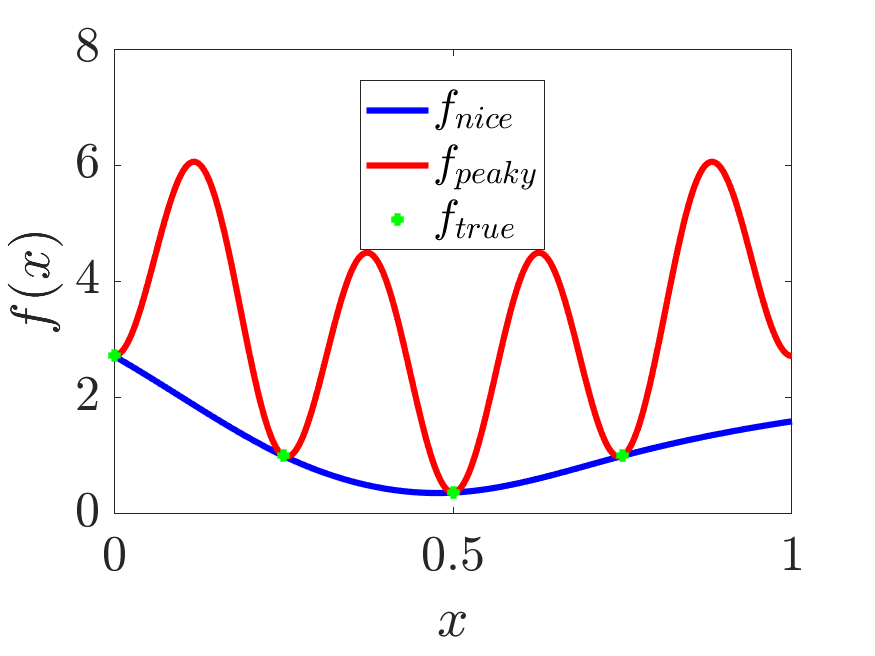
\includegraphics[width=0.9\linewidth]{cone_bayes_f_real}
	%\end{subfigure}
	\caption{Example integrands 1) $f_{true}$ true integrand, 2) $f_{nice}$ a smooth function, and 3) $f_{peaky}$ a peaky function, all have the same values at $\{\vx_i\}_{i=1}^n$.}
	\label{fig:cone_bayes_functions}
\end{figure}
\begin{figure}[ht]
	\centering
	%\begin{subfigure}[h]{0.48\linewidth}
	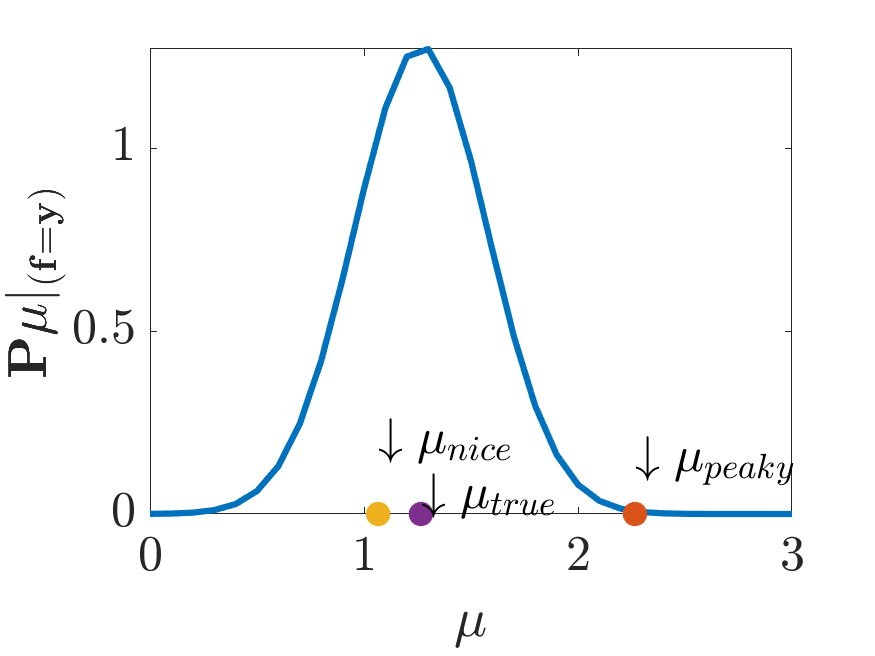
\includegraphics[width=0.9\linewidth]{cone_bayes_mu_pdf}
	%\end{subfigure}
	\caption{Probablity distributions showing the relative position integral of a smooth and a peaky function. $f_{nice}$ lies within the center 99\% of the confidence interval, and $f_{peaky}$ lies on the outside of 99\% of  the confidence interval.\JRNote{Use standard deviation $\sigma$ in x-axis.  $f_{nice}$ using kernel approximation} }
	\label{fig:cone_bayes_posterior}
\end{figure}


As shown in \figref{fig:cone_bayes_functions}, sampled function values $\{f(\vx_i)\}_{i=1}^n$ from a smooth integrand $f_{true}$ are shows as dots. One can imagine these samples $\{f(\vx_i)\}_{i=1}^n$ were obtained from $f_{nice}$, a moderately smoother function or from $f_{peaky}$ a highly oscillating function.

When using $n=16$ rank-1 lattice points and $r=1$ shift-invariant kernel, we get the posterior distribution of $\mu$ as shown in \figref{fig:cone_bayes_posterior}. The true integral value is shown as $\mu_{true}$ which is at the center of the plot. The integral of the peaky function $f_{peaky}$ almost lies outside of the 99\% of the credible interval given by \eqref{eqn_prob_CI_MLE}, whereas the $\mu_{nice}$ falls within.



\Section{The automatic Bayesian cubature algorithm} 
\label{sec:bayes_cubature_algo}

The previous section presents three credible intervals, \eqref{eqn_prob_CI_MLE}, \eqref{eqn_prob_CI_full}, and \eqref{GCVCI}, for the $\mu$, the desired integral.  Each credible interval is based on different assumptions about the hyperparameters $m$, $s$, and $\vtheta$.  We stress that one must estimate these hyperparameters or assume a prior distribution on them because the credible intervals are used as stopping criteria for our cubature rule.  Since a credible intervals makes a statement about a typical function---not an outlier---one must try to ensure that the integrand is a typical draw from the assumed Gaussian process.

Our  Bayesian cubature algorithm increases the sample size until the width of the credible interval is small enough.  This is accomplished through successively doubling the sample size.  The steps are detailed in Algorithm \ref{algorithm1}.

\algnewcommand{\IIf}[1]{\State\algorithmicif\ #1\ \algorithmicthen\ }
\algnewcommand{\IElse}{\unskip\ \algorithmicelse\ }
\algnewcommand{\EndIIf}{\unskip\ \algorithmicend\ \algorithmicif}


\begin{algorithm}
\caption{Automatic Bayesian Cubature}\label{algorithm1}
  \begin{algorithmic}[1]
  	\Require a generator for the sequence
  	$\vx_1, \vx_2, \ldots$; 
  	a black-box function, $f$; 
  	an absolute error tolerance,
  	$\varepsilon>0$; the positive initial sample size, $n_0$;
  	the maximum sample size $n_{\textup{max}}$
  	
      \State $n \gets n_0, \; n' \gets 0, \; \err \gets \infty$
      
      \While{$\err > \varepsilon$ and $n \le n_{\textup{max}}$}
      
        \State\label{LoopStart}Generate $\{ \vx_i\}_{i=n' + 1}^{n}$ and sample $\{f(\vx_i)\}_{i=n'+1}^{n}$
        \State Compute $\vtheta$ by \eqref{eqn:thetaMLE} or \eqref{vthetaGCV}
        \State Compute $\err$  according to \eqref{eqn:errMLE}, \eqref{FJH:eq:errFull}, or \eqref{GCVerr}
        
       	\State	$n' \gets n, \; n \gets 2n'$
        
        \EndWhile
        
        \State Sample size to compute $\hmu$, $n \gets n'$
        \State Compute $\hmu$, the approximate integral,   according to \eqref{eqn:cubMLE} or \eqref{eqn:muCV}
      \State \Return $\hmu, \; n$  and $\err$
  \end{algorithmic}
\end{algorithm}

\Section{Example with the Mat\'ern kernel} \label{MVN_example}

To demonstrate automatic Bayesian cubature consider a Mat\'ern covariance kernel:
\begin{align*}
C_{\theta}(\vx, \vt) = \prod_{k=1}^d \exp(-\theta|\vx_k-\vt_k|)(1+\theta |\vx_k-\vt_k|).
\end{align*}
Also, consider the integration problem of evaluating  \emph{multivariate normal probabilities}:
\begin{equation}
\label{eqn:GaussDef}
\mu = \int_{(\va,\vb)} \frac{\exp\bigl(- \frac 12 \vt^T \mSigma^{-1} \vt \bigr)}{\sqrt{(2 \pi)^d \det(\mSigma)}} \, \dvt,
\end{equation}
where $(\va,\vb)$ is a finite, semi-infinite or infinite box in $\reals^d$.  This integral does not have an analytic expression for general $\mSigma$, so cubatures are required.  

Genz \cite{Gen93} introduced a variable transformation to transform \eqref{eqn:GaussDef} into an integral on the unit cube.  Let $\mSigma= \mL \mL^T$ be the Cholesky decomposition where $\mL = (l_{jk})_{j,k=1}^d$ is a lower triangular matrix.  Iteratively define
\begin{align*}
\alpha_1 = \Phi(a_1), 
&\qquad
\beta_1 = \Phi(b_1),
\\
\alpha_j(x_1,...,x_{j-1}) &= 
\Phi
\left(
\frac{1}{l_{jj}} 
\left(
a_j - \sum_{k=1}^{j-1} l_{jk} \Phi^{-1}(\alpha_k + x_k(\beta_k-\alpha_k))
\right)
\right), \quad j=2,...,d,
\\
\beta_j(x_1,...,x_{j-1}) &= 
\Phi
\left(
\frac{1}{l_{jj}} 
\left(
b_j - \sum_{k=1}^{j-1} l_{jk} \Phi^{-1}(\alpha_k + x_k(\beta_k-\alpha_k))
\right)
\right), \quad j=2,...,d,
\end{align*}
\begin{align}
\label{eqn:fGenzdef}
f_{\text{Genz}}(\vx) = \prod_{j=1}^d [\beta_j(\vx) - \alpha_j(\vx)].
\end{align}
where $\Phi$ is the cumulative standard normal distribution function.  Then, $\mu = \int_{[0,1]^{d-1}} f_{\text{Genz}}(\vx) \, \dvx$.

\begin{figure}
	% \captionsetup[subfigure]{labelformat=empty}
	%\begin{subfigure}[h]{0.48\linewidth}
	%	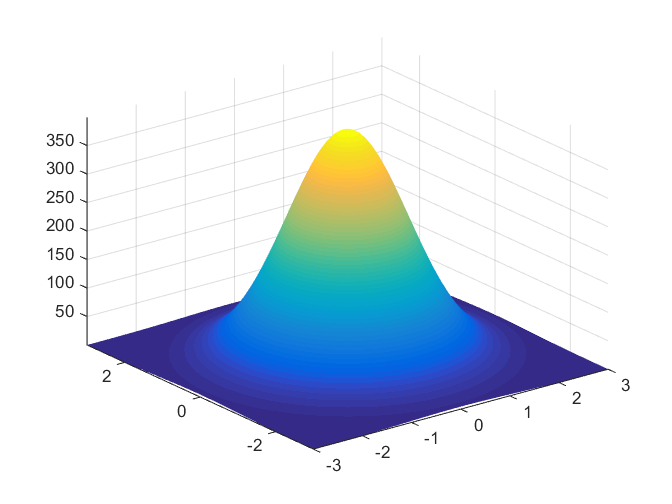
\includegraphics[width=1.1\linewidth]{Plotting_gaussian}
	%\end{subfigure}
	\centering
	%\begin{subfigure}[h]{0.48\linewidth}
		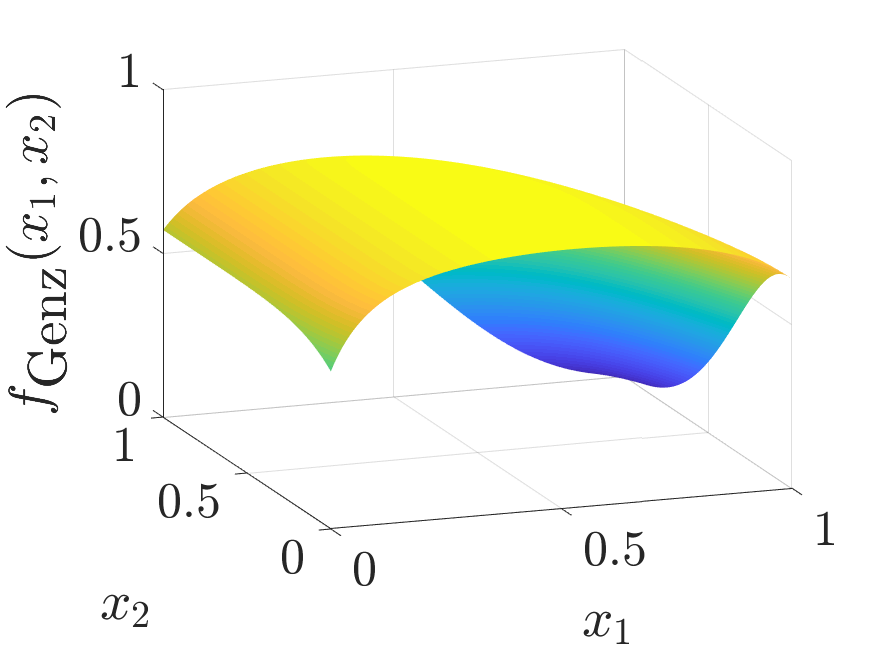
\includegraphics[width=0.9\linewidth]{GenzFunc_varTx_none}
	%\end{subfigure}
	\caption{The $d=3$ multivarivate normal probability transformed to an integral of $f_{\text{Genz}}$ with  $d=2$.}
	\label{fig:MVN_Genz}
\end{figure}

We use the following parameter values in the simulation: 
\begin{equation*}
d = 3, \quad \va = \begin{pmatrix}
-6 \\ -2 \\ -2
\end{pmatrix}, \quad 
\vb = \begin{pmatrix}
5 \\ 2 \\ 1
\end{pmatrix} , \quad 
\mL = \begin{pmatrix}
4 & 1 & 1 \\ 0 & 1 & 0.5 \\ 0 & 0 & 0.25
\end{pmatrix}.
\end{equation*}

\iffalse
\begin{figure}
\captionsetup[subfigure]{labelformat=empty}
\centering
\begin{subfigure}[h]{0.45\linewidth}
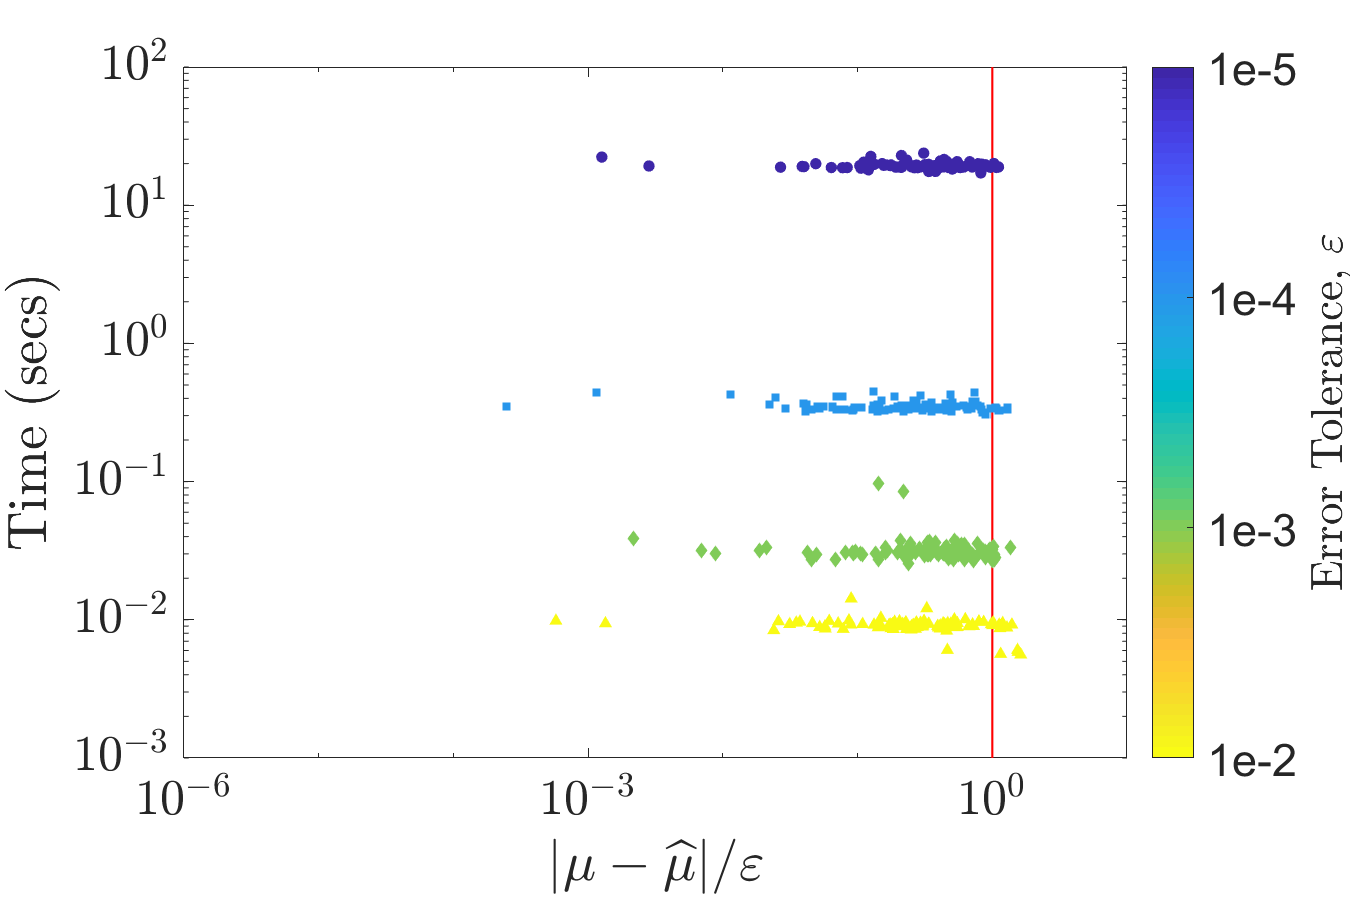
\includegraphics[width=1.1\linewidth]{MVN_guaranteed_time_Matern_d2_2018-Aug-31}
\end{subfigure}
\centering
\begin{subfigure}[h]{0.45\linewidth}
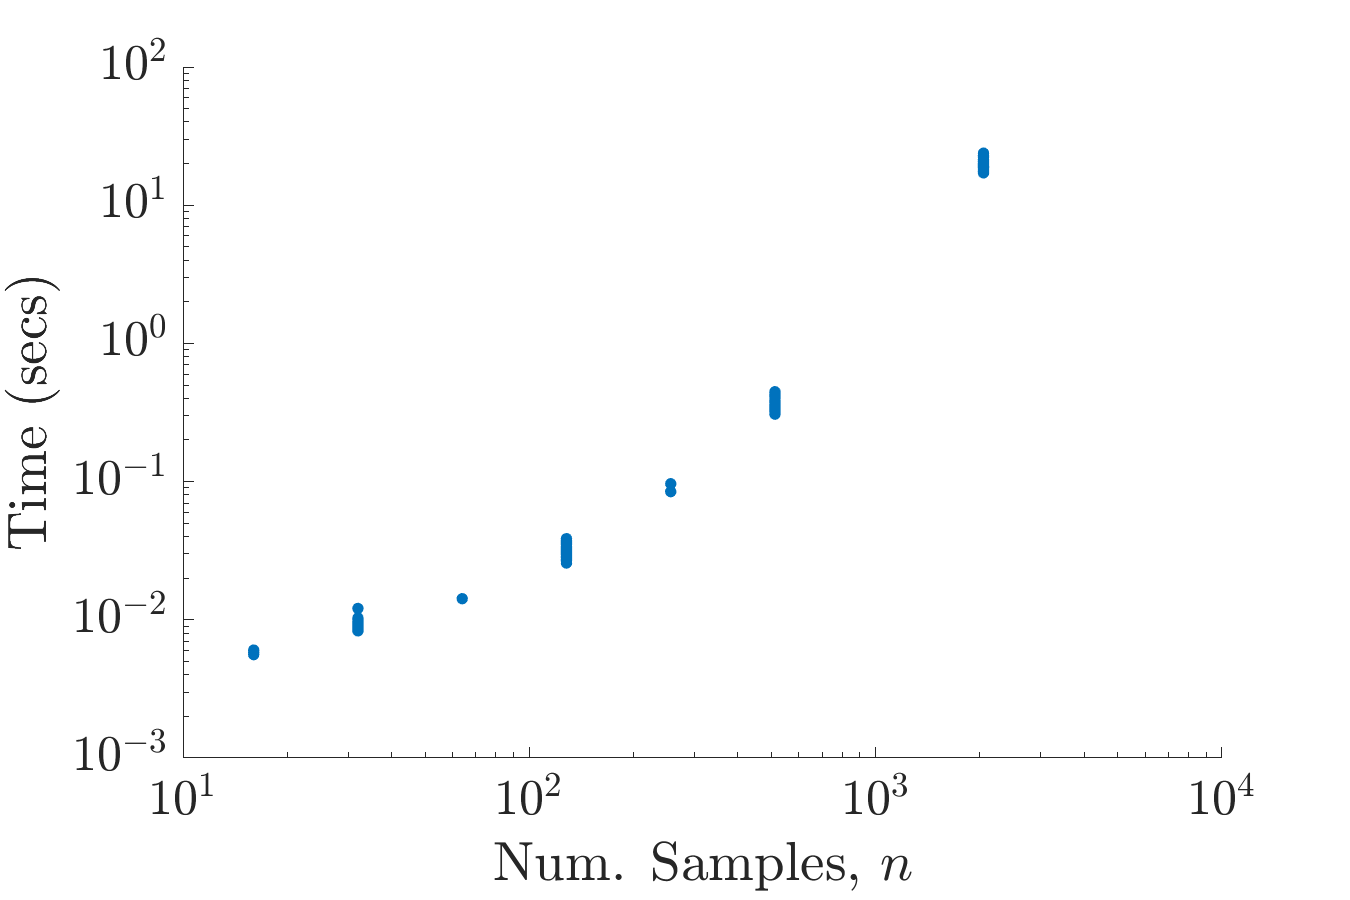
\includegraphics[width=1.1\linewidth]{MVN_rapid_n_vs_time_Matern_d2_2018-Aug-31}
\end{subfigure}
\caption{Multivariate Normal probability estimated using Mat\'ern kernel in d=2 using empirical stopping criterion. Top: Guaranteed integration within error tolerance $\varepsilon$. Bottom: Computation time rapidly increases with increase of $n$}
\label{fig:MVN_Metern_d2b2}
\end{figure}
\fi

\begin{figure}
	\centering
	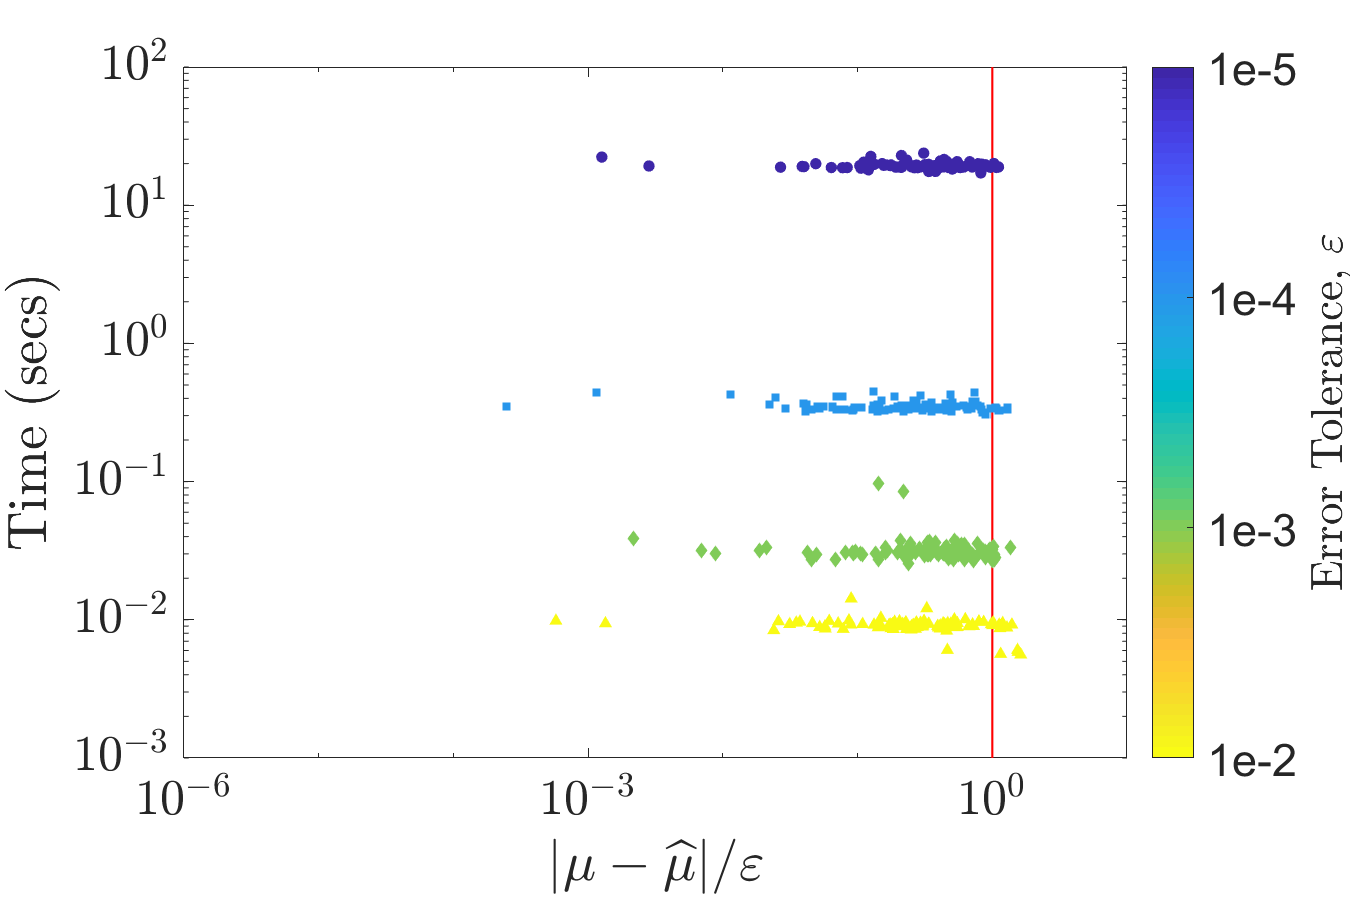
\includegraphics[width=0.9\linewidth]{MVN_guaranteed_time_Matern_d2_2018-Aug-31}
	\caption{Multivariate Normal probability: Guaranteed integration using Mat\'ern kernel in $d=2$ using empirical stopping criterion within error tolerance $\varepsilon$.}
	\label{fig:MVN_Metern_d2b2}
\end{figure}
\begin{figure}
	\centering
	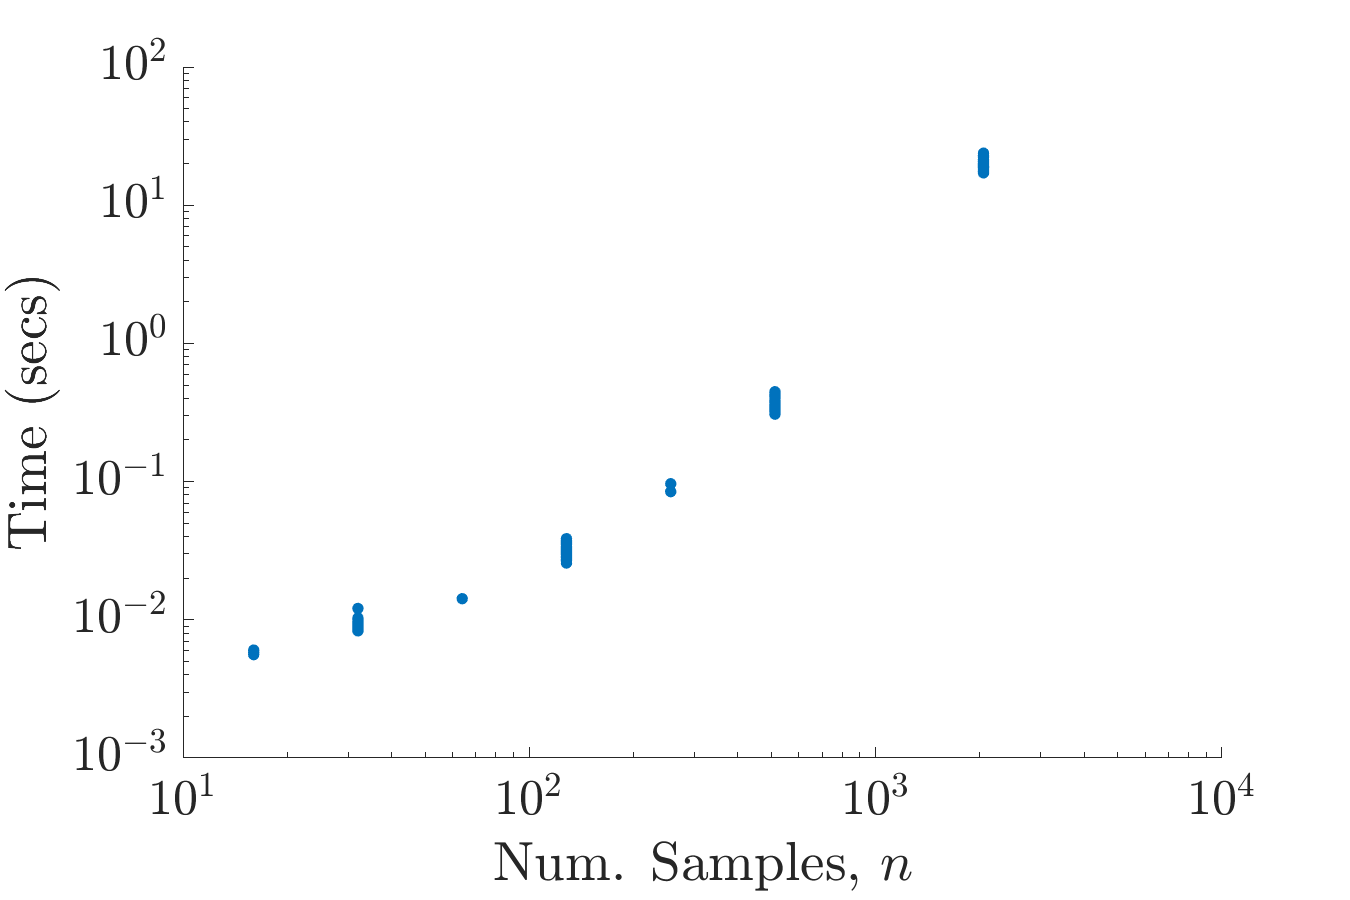
\includegraphics[width=0.9\linewidth]{MVN_rapid_n_vs_time_Matern_d2_2018-Aug-31}
	\caption{Multivariate Normal probability estimated using Mat\'ern kernel in $d=2$ using empirical stopping criterion. Computation time rapidly increases with increase of $n$}
	\label{fig:MVN_Metern_d2b2_time_growth}
\end{figure}

%with Intel i7 3630QM and 16GB RAM memory
On our test computer, it took more than an hour to compute $\hmu_n$ with $n=2^{14}$. As shown in Figure \ref{fig:MVN_Metern_d2b2}, computation time increases rapidly with $n$. 
Especially, maximum likelihood estimation of $\vtheta$, which needs the objective function, is the most time consuming of all. 
Because the objective function needs to be computed multiple times in every iteration to find its minimum. 
Not only the computational cost increases, also the $\mC$ becomes highly ill-conditioned with increasing $n$.
So, our algorithm in the current form is not straightaway usable for any practical applications.


\Chapter{Fast Automatic Bayesian Cubature}
%\Section{Fast Automatic Bayesian Cubature}
\label{sec:fast_BC}

The generic automatic Bayesian cubature algorithm described in the previous section requires $\Order(n^3)$ operations to estimate $\vtheta$, compute the credible interval width, and compute the cubature.  This section explains how to speed up the calculations. A key is to choose kernels that match the design, $\{\vx_i\}_{i=1}^n$, so that the vector-matrix operations required by Bayesian cubature can be accomplished using fast transforms at a cost of $\Order(n \log(n))$.

\Section{Fast Transform Kernel}

We make some assumptions about the relationship between the covariance kernel and the design, which will be shown to hold in Section \ref{sec:shift_invariant_kernel} for rank-1 lattices and shift-invariant kernels.  First we introduce the notation
\begin{align}
\nonumber
\mC &= \Big(C_\vtheta(\vx_i,\vx_j)\Big)_{i,j=1}^n  = (\vC_1,...,\vC_n) 
\\
\label{eqn:ftk_factor}
&= \frac 1n \mV \mLambda \mV^H , 
\quad \quad \mV^H = n \mV^{-1}, \\
\nonumber
\mV &= (\vv_1,...,\vv_n)^T = (\vV_1,...,\vV_n) \\
\nonumber
\mC^p  &= \frac 1n \mV \mLambda^{p} \mV^H, \qquad \forall p \in \integers,
\end{align}
where $\mV^H$ is the Hermitian of $\mV$.  The columns of matrix $\mV$ are eigenvectors of $\mC$, and $\mLambda$ is a diagonal matrix of eigenvalues of $\mC$.
For any $n \times n$ vector $\vb$, define the notation  $\widetilde{\vb} := \mV^H \vb$.

We make three assumptions that allow the fast computation:
\begin{subequations} \label{fastcompAssump}
	\begin{gather}
	\label{fastcompAssumpA}
	\mV \text{ may be identified analytically}, \\
	\label{fastcompAssumpB}
	\vv_1 = \vV_1 = \vone, \\
	\label{fastcompAssumpC}
	\mV^H \vb  \text{ requires only $\Order(n \log(n))$ operations } \forall \vb.
	\end{gather}
\end{subequations}
We call the transformation $\vb \mapsto \mV^H \vb$ a \emph{fast transform} and $C_\vtheta$ a \emph{fast transform kernel}.  

Under assumptions \eqref{fastcompAssump} the eigenvalues may be identified as the fast transform of the first column of $\mC$:
\begin{align}
\nonumber
\vlambda 
& = \begin{pmatrix}
\lambda_1, &\dots, &\lambda_n
\end{pmatrix}^T = \mLambda \vone = \mLambda \vv_1^* 
= \underbrace{\left( \frac 1n \mV^H  \mV \right) }_{\mathsf{I}} \mLambda \vv_1^* \\
&= \mV^H \left( \frac 1n \mV \mLambda \vv_1^* \right)
= \mV^H \vC_1 =  \widetilde{\vC}_1.
\label{eqn:fast_transform_to_eigvalues}
\end{align}
Also note that the fast transform of $\vone$ has a simple form
\begin{align*} 
\widetilde{\vone}
& = \mV^H \vone = \mV^H \vV_1 = \begin{pmatrix}n, & 0, & \dots, & 0 \end{pmatrix}^T.
\label{eqn:fast_transform_one}
\end{align*}

Many of the terms that arise in the calculations in  Algorithm \ref{algorithm1} take the form $\va^T\mC^{p}\vb$ for real $\va$ and $\vb$ and integer $p$.  These can be calculated via the transforms $\widetilde{\va} = \mV^H \va$ and $\widetilde{\vb} = \mV^H \vb$ as 
\begin{equation*}
\va^T\mC^p\vb = \frac 1n \va^T \mV \mLambda^p \mV^H \vb
= \frac 1n \widetilde{\va}^H\mLambda^p \widetilde{\vb}
= \frac 1n \sum_{i=1}^n \lambda_i^p \widetilde{a}_i^* \widetilde{b}_i, 
\end{equation*}
In particular,
\begin{align*}
\vone^T\mC^{-p}\vone & = \frac{n}{\lambda_1^p},
&
\vone^T\mC^{-p}\vy &= \frac{\widetilde{y}_1}{\lambda_1^p},
\\
\vy^T\mC^{-p} \vy &= \frac 1n \sum_{i=1}^n \frac{\abs{\widetilde{y}_i}^2}{\lambda_i^p},
&
\vc^T\mCInv \vone &= \frac{\widetilde{c}_1}{\lambda_1},\\
\vc^T\mCInv \vy &= \frac 1n \sum_{i=1}^n \frac{\widetilde{c}_i^* \widetilde{y}_i}{\lambda_i}, & 
\vc^T\mCInv \vc &= \frac 1n \sum_{i=1}^n \frac{\abs{\widetilde{c}_i}^2}{\lambda_i},
\end{align*}
where $\widetilde{\vy} = \mV^H \vy$ and 
$\widetilde{\vc} = \mV^H \vc$.  For any real $\vb$, with $\widetilde{\vb} = \mV^H\vb$, it follows that $\widetilde{b}_1$ is real since the first row of $\mV^H$ is $\vone$.

The covariance kernel used in practice also may satisfy an additional assumption:
\begin{equation} \label{addAssump}
\int_{[0,1]^d} C(\vt,\vx) \, \D \vt = 1 \qquad \forall \vx \in [0,1]^d,
\end{equation}
which implies that $c_0 = 1$ and $\vc = \vone$.  Under \eqref{addAssump}, the expressions above may be further simplified:
\begin{equation*}
\vc^T\mCInv \vone =
\vc^T\mCInv \vc = \frac{n}{\lambda_1}.
\end{equation*}


\Section{Empirical Bayes}

Under assumptions \eqref{fastcompAssump}, the empirical Bayes parameters in \eqref{eqn_m_MLE}, \eqref{eqn_s2_MLE}, \eqref{eqn:thetaMLE} \eqref{eqn:cubMLE}, and \eqref{eqn:errMLE} can be expressed in terms of the fast transforms of the function data, the first column of the Gram matrix, and $\vc$ as follows:
\begin{align}
\nonumber
m_\MLE &=  \frac{\widetilde{y}_1}{n} = \frac 1n \sum_{i=1}^n y_i,
\\
\nonumber
s^2_\MLE 
& =
\frac{1}{n^2} 
\sum_{i=2}^n \frac{\abs{\widetilde{y}_i}^2}{\lambda_i}, \\
\label{eqn_MLE_loss_func_optimized_2}
\vtheta_\MLE
&= 
\argmin_{\vtheta}
\left[
\log\left(
\sum_{i=2}^n \frac{\abs{\widetilde{y}_i}^2}{\lambda_i}
\right)   + 
\frac{1}{n}\sum_{i=1}^n \log(\lambda_i)
\right],
\\
\nonumber
\hmu_\MLE  &= 
\frac{\widetilde{y}_1}{n} +
\frac 1n \sum_{i=2}^n \frac{ \widetilde{c}_i^* \widetilde{y}_i}{\lambda_i}, \\
\nonumber
\err_\MLE  &
=
\frac{2.58}{n}\sqrt{
	\sum_{i=2}^{n} \frac{\abs{\widetilde{y}_i}^2}{\lambda_i}  
	\,
	\left( c_0 - \frac 1n \sum_{i=1}^n \frac{\abs{\widetilde{c}_i}^2}{\lambda_i} \right) 
},
\end{align}
Since all the quantities on the right hand sides can be obtained in $\Order(n \log(n))$ operations by fast transforms, the left hand sides are all computable using the asymptotic computational cost.

Under the further assumption \eqref{addAssump} it follows that 
\begin{align}
\nonumber
\hmu_\MLE  &= 
\frac{\widetilde{y}_1}{n} = \frac 1n \sum_{i=1}^n y_i,\\
\label{eq:errMLEAllAsump}
\err_\MLE  &
=
\frac{2.58}{n}\sqrt{
	\sum_{i=2}^{n} \frac{\abs{\widetilde{y}_i}^2}{\lambda_i}  
	\,
	\left( 1 -  \frac{n}{\lambda_1} \right) 
}.
\end{align}
Thus, in this  case $\hmu$ is simply the sample mean.



\Subsection{Gradient of the objective function using fast transform} \label{deriv_obj_func_MLE} 
If $\mV$ does not depend on $\vtheta$ then one can fast compute the derivative of matrix $\mC$. Starting from the definition \eqref{eqn:ftk_factor} and taking derivative w.r.t. $\theta_j$, 
\begin{align*}
\displaystyle \frac{\partial \mC}{\partial \theta_j} 
& = \frac 1n \mV \frac{\partial {\mLambda}}{\partial \theta_j} \mV^H
= \frac 1n \mV \bar{\mLambda}_{(j)} \mV^H,
\\
& \text{where} \quad \bar{\mLambda}_{(j)} = \diag(\bar{\vlambda}_{(j)}), \quad \text{and}
\\
&  \quad \bar{\vlambda}_{(j)} = \frac{\partial \vlambda}{\partial \theta_j} = \left( \frac{\partial \lambda_i}{\partial \theta_j} \right)_{i=1}^n 
 = \left( \frac{\partial }{\partial \theta_j} \mV^H {\vC_1} \right)
 = \mV^H \left( \frac{\partial }{\partial \theta_j} {C_\vtheta(\vx_1,\vx_i)} \right)_{i=1}^n.
\end{align*}
where we used the fast transform property \eqref{eqn:fast_transform_to_eigvalues}.
We use the notation $\bar{\vlambda}_{(j)} = \mV^H \bar{\vC_1}_{(j)}$,  where $\bar{\vC}_{1(j)}$ denotes the first row of the gram matrix after taking derivative, i.e.
\begin{align*}
\bar{\vC}_{1{(j)}} = \left(\frac{\partial }{\partial{\theta}_j} C_\vtheta(\vx_1,\vx_i) \right)_{i=1}^n.
\end{align*}
The goal is to find derivative of the objective function. First, let's rewrite the objective function from \eqref{eqn_MLE_loss_func_optimized_2},
\begin{align*}
\mathcal{L}(\vtheta | \vy) &= 
\underbrace{\frac{1}{n}  \log(\det\, \mC)}_{\mathcal{L}_{\abs{\mC}}} + \underbrace{\log\left((\vy-m_\MLE\vone)^T\mCInv(\vy-m_\MLE\vone) \right)}_{\mathcal{L}_{\vy}}
\\ &=: \mathcal{L}_{\abs{\mC}} + \mathcal{L}_{\vy}
\end{align*}
Now, take the derivative
\begin{align*}
\frac{\partial}{\partial \theta_j} \mathcal{L}(\vtheta | \vy)
&=  \frac{\partial}{\partial \theta_j} \mathcal{L}_{\abs{\mC}} + \frac{\partial}{\partial \theta_j} \mathcal{L}_{\vy}
\end{align*}
Let's tackle the individual terms
\begin{align*}
\frac{\partial}{\partial \theta_j} \mathcal{L}_{\abs{\mC}} &= \frac{\partial}{\partial \theta_j}  \frac{1}{n} \log(\det\, \mC) 
\\ & = \frac 1n \trace{\left( \mCInv \frac{\partial \mC}{\partial \vtheta_j} \right)}
 = \frac{1}{n}
\trace{\left( \mV {\mLambda}^{-1} \mV^H
\frac 1n \mV \overline{\mLambda}_{(j)} \mV^H
\right)}
\\
& = \frac{1}{n}
\trace{\left(
	 \mV {\mLambda}^{-1}  \overline{\mLambda}_{(j)} \mV^H
	\right)}, \quad \text{where we used } \; \mV^H \mV = n
\\
& =\frac{1}{n}
\trace{\left(
	 \mV \;
	\diag\left( \frac{\overline{\lambda}_{i(j)}}{\lambda_i} \right)_{i=1}^n \mV^H
	\right)}
= \frac{1}{n} \sum_{i=1}^{n} \frac{\overline{\lambda}_{i(j)}}{\lambda_i}
\end{align*}
where we used the fact from \cite{Hig08}
\begin{align*}
\log(\det\, \mC)  = \trace{ (\log( \mC)) }.
\end{align*}
Part of the $\mathcal{L}_{\vy}$ was already simplified using the fast transform,
\begin{align*}
{(\vy-m_\MLE\vone)^T\mCInv(\vy-m_\MLE\vone)} = \frac{1}{n} \sum_{i=2}^n \frac{\abs{\widetilde{y}_i}^2}{\lambda_i}.
\end{align*}
Using the above result,
\begin{align*}
\frac{\partial}{\partial \theta_j} \mathcal{L}_{\vy} 
&= \frac{\partial}{\partial \vtheta_j} \log\left(\frac{1}{n} \sum_{i=2}^n \frac{\abs{\widetilde{y}_i}^2}{\lambda_i} \right) 
\\ 
&= \left(\frac{1}{n} \sum_{i=2}^n \frac{\abs{\widetilde{y}_i}^2}{\lambda_i}\right)^{-1}
\;
\frac{\partial}{\partial \vtheta_j} \left(\frac{1}{n} \sum_{i=2}^n \frac{\abs{\widetilde{y}_i}^2}{\lambda_i} \right) 
\\ &= \left(
\frac{1}{n} \sum_{i=2}^n \frac{\abs{\widetilde{y}_i}^2}{\lambda_i} \right)^{-1} \frac{1}{n} \sum_{i=2}^n \frac{\abs{\widetilde{y}_i}^2}{\lambda_i^2}
\left( -\frac{\partial \lambda_i}{\partial \vtheta_j} \right)
\\ &= -\left(
\sum_{i=2}^n \frac{\abs{\widetilde{y}_i}^2}{\lambda_i} \right)^{-1} 
\left( \sum_{i=2}^n \abs{\widetilde{y}_i}^2 \frac{ \bar{ \lambda}_{i(j)} }{\lambda_i^2}
 \right).
\end{align*}
Finally, using the above results
\begin{align*}
\frac{\partial}{\partial \theta_j} \mathcal{L}(\vtheta | \vy) 
&=  \frac 1n \sum_{i=1}^{n} \frac{\bar{\lambda}_{i(j)}}{\lambda_i}
- \left({ \sum_{i=2}^n \frac{\abs{\tvy_i}^2 \bar{\lambda}_{i(j)}}{\lambda_i^2}}\right)
\left( {\sum_{i=2}^n \frac{\abs{\tvy_i}^2}{\lambda_j}} \right)^{-1}.
\end{align*}
If $m=0$ assumption can be made
\begin{align*}
\frac{\partial}{\partial \theta_j} \mathcal{L}(\vtheta | \vy) 
&=  \frac 1n \sum_{i=1}^{n} \frac{\bar{\lambda}_{i(j)}}{\lambda_i}
- \left({ \sum_{i=1}^n \frac{\abs{\tvy_i}^2 \bar{\lambda}_{i(j)}}{\lambda_i^2}}\right)
\left( {\sum_{i=1}^n \frac{\abs{\tvy_i}^2}{\lambda_j}} \right)^{-1}.
\end{align*}

\Section{Full Bayes}

For the full Bayes approach the cubature is the same as for empirical Bayes.  We also defer to empirical Bayes to estimate the parameter $\vtheta$.  The width of the confidence interval is $\err_{\textup{full}} 
:= t_{n_j-1,0.995} \hsigma_{\textup{full}}$, where $\hsigma_{\textup{full}}^2$ can also be computed swiftly under assumptions \eqref{fastcompAssump}:
\begin{align*} %\label{FJH:eq:signmaFull}
\widehat{\sigma}^2_{\textup{full}} =
\frac{1}{n(n-1)} \sum_{i=2}^n \frac{\abs{\widetilde{y}_i}^2}{\lambda_i}
\left[\frac{\lambda_1}{n}{\left(1 - \frac{\widetilde{c}_1}{\lambda_1}\right)^2} + \left(c_0  - \frac 1n \sum_{i=1}^n \frac{\abs{\widetilde{c}_i}^2}{\lambda_i}\right) \right],
\end{align*}
Under assumption \eqref{addAssump} further simplification can be made:
\begin{equation*} %\label{FJH:eq:signmaFullSimple}
\widehat{\sigma}^2_{\textup{full}}
=
\frac{1}{n(n-1)} \sum_{i=2}^n \frac{\abs{\widetilde{y}_i}^2}{\lambda_i} \, \left(\frac{\lambda_1}{n}  - 1  \right),
\end{equation*}
It follows that
\begin{equation} \label{FJH:eq:errFullSimple}
\err_{\textup{full}}
=
t_{n_j-1,0.995}
\sqrt{\frac{1}{n(n-1)} \sum_{i=2}^n \frac{\abs{\widetilde{y}_i}^2}{\lambda_i} \, \left(\frac{\lambda_1}{n}  - 1  \right)}.
\end{equation}


\Section{Generalized Cross-Validation}

GCV yields a different cubature, which nevertheless can also be computed quickly using the fast transform.  Under assumptions \eqref{fastcompAssump}:
\begin{align}
\nonumber
m_{\textup{GCV}} & = m_\MLE =  \frac{\widetilde{y}_1}{n} = \frac 1n \sum_{i=1}^n y_i,\\
\nonumber 
s^2_{\textup{GCV}} & : =  \frac 1{n} \sum_{i=2}^n \frac{\abs{\widetilde{y}_i}^2}{\lambda_i^2}  \left [ \sum_{i=1}^n \frac{1}{\lambda_i} \right]^{-1}, \\
\label{thetaGCV}
\vtheta_{\GCV} 
&= \argmin_\vtheta \left[ \log \left ( \sum_{i=2}^n \frac{\abs{\widetilde{y}_i}^2}{\lambda_i^2} 
\right) -2\log\left( \sum_{i=1}^n \frac{1}{\lambda_i} \right)
\right], \\
\nonumber
\hmu_{\GCV}
&= \hmu_\MLE  = \frac{\widetilde{y}_1}{n} +
\frac 1n \sum_{i=2}^n \frac{ \widetilde{c}_i^* \widetilde{y}_i}{\lambda_i}, \\
\nonumber
\err_{\textup{GCV}} & =
\frac{2.58}{n}\left\{\sum_{i=2}^n \frac{\abs{\widetilde{y}_i}^2}{\lambda_i^2}  \left [ \frac 1n \sum_{i=1}^n \frac{1}{\lambda_i} \right]^{-1}  \times
\left( c_0 - \frac 1n \sum_{i=1}^n \frac{\abs{\widetilde{c}_i}^2}{\lambda_i} \right) 
\right\}^{1/2}.
\end{align}
Moreover, under further assumption \eqref{addAssump} it follows that 
\begin{align}
\nonumber %\label{muhatGCV-FB-MLE-Simple}
\hmu_{\textup{GCV}}
&= \hmu_\MLE = \hmu_{\textup{full}} =
\frac{\widetilde{y}_1}{n} = \frac 1n \sum_{i=1}^n y_i,\\
\label{errGCVSimple}
\err_{\textup{GCV}} & =
\frac{2.58}{n}\left\{\sum_{i=2}^n \frac{\abs{\widetilde{y}_i}^2}{\lambda_i^2}  \left [ \frac 1n \sum_{i=1}^n \frac{1}{\lambda_i} \right]^{-1}  \times
\left( 1 -  \frac{n}{\lambda_1} \right)  
\right\}^{1/2}.
\end{align}
In this case too, $\hmu$ is simply the sample mean.


\Subsection{Derivative of the loss function}
Using the results obtained from the previous section, we can reduce the computational cost of the derivative of the loss function,
\begin{align*}
\mathcal{L}(\vtheta | \vy)_\GCV
&= \log \left ( \sum_{i=2}^n \frac{\abs{\widetilde{y}_i}^2}{\lambda_i^2} 
\right) -2\log\left( \sum_{i=1}^n \frac{1}{\lambda_i} \right)
\end{align*}
Using the similar techniques from \secref{deriv_obj_func_MLE}
\begin{align*}
& \frac{\partial}{\partial \theta_j}  \mathcal{L}(\vtheta | \vy)_\GCV
\\
&= \left ( \sum_{i=2}^n \frac{\abs{\widetilde{y}_i}^2}{\lambda_i^2} \right)^{-1}
\frac{\partial}{\partial \theta_j} \left ( \sum_{i=2}^n \frac{\abs{\widetilde{y}_i}^2}{\lambda_i^2} \right)
 -2 \left( \sum_{i=1}^n \frac{1}{\lambda_i} \right)^{-1}
\frac{\partial}{\partial \theta_j} \left( \sum_{i=1}^n \frac{1}{\lambda_i} \right)
\\
&= \left ( \sum_{i=2}^n \frac{\abs{\widetilde{y}_i}^2}{\lambda_i^2} \right)^{-1}
 \left ( \sum_{i=2}^n \frac{\abs{\widetilde{y}_i}^2}{\lambda_i^3} (-2) \frac{\partial\lambda_i}{\partial \theta_j}  \right)
\\ & \hspace{4cm} 
-2 \left( \sum_{i=1}^n \frac{1}{\lambda_i} \right)^{-1}
\left( \sum_{i=1}^n \frac{1}{\lambda_i^2} (-1)\frac{\partial \lambda_i}{\partial \theta_j}  \right)
\\
&= -2 \left ( \sum_{i=2}^n \frac{\abs{\widetilde{y}_i}^2}{\lambda_i^2} \right)^{-1}
\left ( \sum_{i=2}^n \frac{\abs{\widetilde{y}_i}^2 \bar{\lambda}_{i(j)} }{\lambda_i^3}    \right)
+ 2 \left( \sum_{i=1}^n \frac{1}{\lambda_i} \right)^{-1}
\left( \sum_{i=1}^n \frac{\bar{\lambda}_{i(j)} }{\lambda_i^2}  \right)
\end{align*}


\Section{Product kernel}

In this research, We use product kernels in the demonstrations and numerical implementations. They got nice properties which are helpful to obtain analytical results easily. Product kernels are of the form in $d$ dimensions
\begin{align}
\label{eqn:prod_kernel}
C_\vtheta(\vt, \vx) = 
\prod_{l=1}^d \biggl[ 1 - \eta \; \mathfrak{C}(x_l,t_l) \biggr]
\end{align}
% $ C_\vtheta(\vt, \vx) = \prod_{l=1}^d [ 1 - \eta_l \mathfrak{C}(x_l,t_l) ]$
where $\eta$ is called shape parameter and $\mathfrak{C}$ is some positive definite function. The derivative of the product kernel can be obtained easily.

\Subsection{Derivative of the product kernel}
\label{sec:deriv_of_kernel}
We discussed using gradient descent to find optimal shape parameter in  \secref{grad_descent_MLE} which requires the derivative of kernel w.r.t. $\eta$
\begin{align*}
\frac{\partial}{\partial \eta} C_\vtheta(\vt, \vx) 
& =
\frac{\partial}{\partial \eta} 
\prod_{l=1}^d \biggl[
1 - \eta \mathfrak{C}(x_l,t_l) \biggr], % \quad  \mathfrak{C}(x,t) := (-1)^{r} B_{2r}( |{x-t}| \bmod 1 ) 
\\
& = 
\sum_{j=1}^d  
\prod_{l=1, l \neq j}^d \biggl[
1 - \eta \mathfrak{C}(x_l,t_l) \biggr]
\biggl( - \mathfrak{C}(x_j,t_j) \biggr)
\\
& =
\prod_{l=1}^d \biggl[
1 - \eta \mathfrak{C}(x_l,t_l) \biggr]
\sum_{j=1}^d 
\frac{
	\biggl( - \mathfrak{C}(x_j,t_j) \biggr)
}{
	1 - \eta \mathfrak{C}(x_j,t_j) 
}
\\
& =
C_\vtheta(\vt, \vx) 
\frac{1}{\eta}
\sum_{j=1}^d 
\frac{
	\biggl(1 - \eta \mathfrak{C}({x_j,t_j})  - 1 \biggr)
}{
	1 - \eta \mathfrak{C}(x_j,t_j) 
}
\\
& =
C_\vtheta(\vt, \vx) 
\frac{1}{\eta}
\sum_{j=1}^d 
\biggl(
1 - 
\frac{1
}{
	1 - \eta \mathfrak{C}(x_j,t_j) 
}
\biggr)
\\
& =
\frac{d}{\eta} 
\underbrace{
	\left(
	\prod_{l=1}^d \biggl[
	1 - \eta \mathfrak{C}(x_l,t_l) \biggr]
	\right) }_
{ C_\vtheta(\vt, \vx) }
\biggl(
1 - 
\frac{1}{d} \sum_{j=1}^d
\frac{1}
{ 1 - \eta \mathfrak{C}(x_j,t_j) }
\biggr)
\end{align*}

\Subsubsection{When $\eta_j$ fixed per dimension $j$}
In this case, we will have a vector of length $d$ shape parameters. For the dimension $j$,
\begin{align*}
\frac{\partial}{\partial \eta_j} C_\vtheta(\vt, \vx) 
& =
\frac{\partial}{\partial \eta_j} 
\prod_{l=1}^d \biggl[
1 - \eta_l \mathfrak{C}(x_l,t_l) \biggr]
\\
& = 
\prod_{l=1, l \neq j}^d \biggl[
1 - \eta_l \mathfrak{C}(x_l,t_l) \biggr]
\biggl( - \mathfrak{C}(x_j,t_j) \biggr)
\\
& =
\prod_{l=1}^d \biggl[
1 - \eta_l \mathfrak{C}(x_l,t_l) \biggr]
\frac{
	\biggl( - \mathfrak{C}(x_j,t_j) \biggr)
}{
	1 - \eta_j \mathfrak{C}(x_j,t_j) 
}
\\
& =
C_\vtheta(\vt, \vx) 
\frac{1}{\eta_j}
\frac{
	\biggl(1 - \eta_j \mathfrak{C}(x_j,t_j)  - 1 \biggr)
}{
	1 - \eta_j \mathfrak{C}(x_j,t_j) 
}
\\
& =
C_\vtheta(\vt, \vx) 
\frac{1}{\eta_j}
\biggl(
1 - 
\frac{1
}{
	1 - \eta_j \mathfrak{C}(x_j,t_j) 
}
\biggr)
\\
& =
\frac{1}{\eta_j} 
\underbrace{
	\left(
	\prod_{l=1}^d \biggl[
	1 - \eta \mathfrak{C}(x_l,t_l) \biggr]
	\right) }_
{ C_\vtheta(\vt, \vx) }
\biggl(
1 - 
\frac{1}
{ 1 - \eta_j \mathfrak{C}(x_j,t_j) }
\biggr)
\end{align*}
Please note the above derivatives do not depend on $\mathfrak{C}(x,t)$ and most importantly these computations are applicable to any product kernel of the form \eqref{eqn:prod_kernel}.
%$ C_\vtheta(\vt, \vx) = \prod_{l=1}^d [ 1 - \eta_l \mathfrak{C}(x_l,t_l) ]$.

\Subsection{Shape parameter search using steepest descent}
Having obtained the derivative, we can easily implement the steepest descent search introduced in \secref{grad_descent_MLE} 
%\eqref{Dong2017a}
\begin{align*}
\eta^{(j+1)} = \eta^{(j)} - \nu \frac{\partial}{\partial \eta} \mathcal{L}(\vtheta | \vy)
\end{align*}













\Chapter{Integration Lattices and \\ Shift Invariant Kernels}
\label{sec:shift_invariant_kernel}

The preceding sections lay out an automatic Bayesian cubature algorithm whose computational cost is only $\Order(n \log(n))$ if $n$ function values are used.  However, this algorithm relies on covariance kernel functions, $C_{\vtheta}$ and designs, $\{\vx_i\}_{i=1}^n$ that satisfy assumptions \eqref{fastcompAssump}.  
In this chapter, we demonstrate such a covariance kernel and matching design.
When periodic shift-invariant kernels are combined with rank-1 Lattice nodes as design, we get circulant Gram matrix. 
We will also satisfy assumption \eqref{addAssump}.  To make the computations simpler and facilitate the fast transform, it is assumed in this section and the next that $n$ is power of $2$.  


\Section{Extensible Integration Lattice Node Sets}

The design or set of nodes used is defined by a shifted extensible integration lattice node sequence, which takes the form
\begin{equation}
\label{eqn:lattice_gen}
\vx_{i} = \vh \phi(i-1) + \vDelta \mod \vone, \qquad i \in \naturals.
\end{equation} 
Here, $\vh$ is a $d$-dimensional generating vector of positive integers, $\vDelta$ is some point in $[0,1)^d$, often chosen at random, and $\{\phi(i)\}_{i=0}^n$ is the van der Corput sequence, defined by reflecting the binary digits of the integer about the decimal point, i.e., 
\begin{equation} \label{vdCDef}
\begin{array}{r|ccccccccccccc}
i & 0 & 1 & 2 & 3 & 4 &  5 & 6 & 7 & \cdots \\
i & 0_2 & 1_2 & 10_2 & 11_2 & 100_2 & 101_2 & 110_2 & 111_2  & \cdots\\
\toprule
\phi(i) & {}_2.0 &  {}_2.1 & {}_2.01 &  {}_2.11  & {}_2.001 &  {}_2.101 & {}_2.011 &  {}_2.111 & \cdots\\
\phi(i) & 0 &  0.5 &  0.25 & 0.75 &  0.125 & 0.625  &  0.375 & 0.875 & \cdots
\end{array}
\end{equation}

A random shift  $\vDelta$ is added to $\vx_{i}$ to avoid the origin zero in our point set. However, this shift will preserve the discrepancy properties of $\vx_{i}$. These are called rank-1 lattices.
rank-1 lattices with the module one addition have a very desirable group structure that helps to satisfy fast transform kernel assumptions.


An example of $64$ nodes is given in Figure  \ref{latticefig}.  The even coverage of the unit cube is ensured by a well chosen generating vector.  The choice of generating vector is typically done offline by computer search.  See \cite{DicEtal14a} and \cite{HicNie03a} for more on extensible integration lattices. Lattice rules are designed to integrate the class of sinusoidal functions without error.
\begin{figure}[htp]
	\centering
	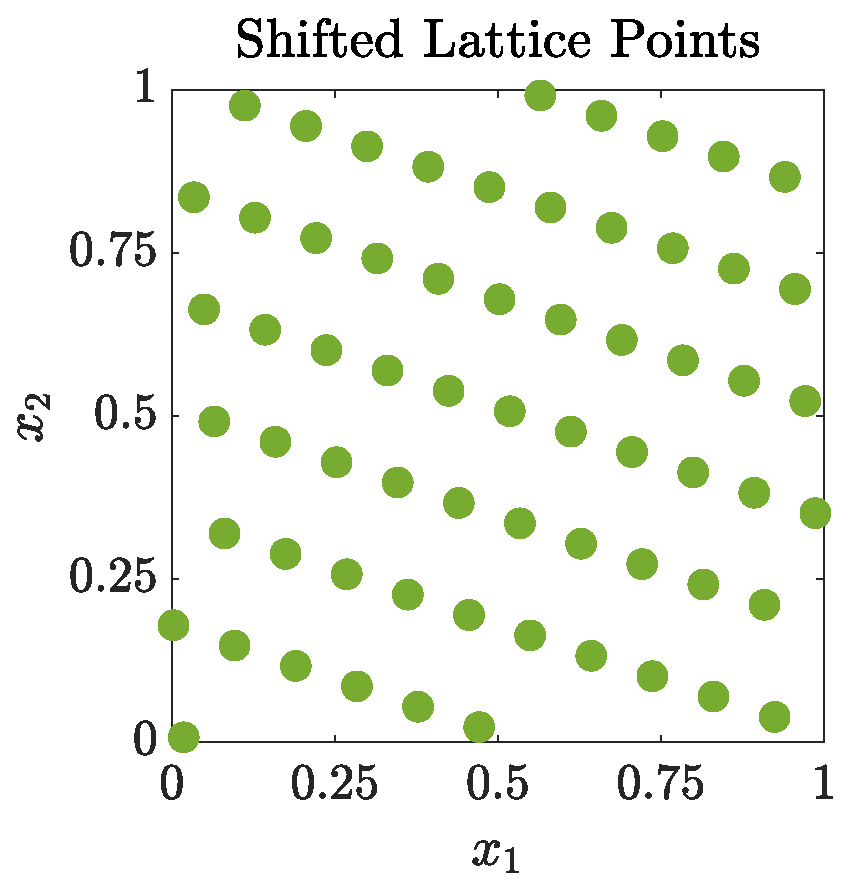
\includegraphics[width=0.7\linewidth]{ShiftedLatticePoints}
	\caption{Example of a shifted integration lattice node set  in $d=2$ \label{latticefig} }
\end{figure}

\Section{Shift Invariant Kernels}\label{sec:shift_invar_kern}

The covariance functions $C$ that match integration lattice node sets have the form
\begin{equation} \label{eq:shInv}
C_{\vtheta}(\vt,\vx) = K_{\vtheta}(\vt - \vx \bmod \vone).
\end{equation}
This is called a \emph{shift invariant kernel} because shifting both arguments of the covariance function by the same amount leaves the value unchanged.   By a proper scaling of the kernel $K_{\vtheta}$ it follows that assumption \eqref{addAssump} is satisfied. Of course, $K_{\vtheta}$ must also be of the form that ensures that $C_{\vtheta}$ is symmetric and positive definite, as assumed in \eqref{FJH:eq:CondPosDef}. 

A family of shift invariant kernels is constructed via even degree Bernoulli polynomials:
\begin{align*}
C_\vtheta(\vx, \vt) := &  \sum_{\vk \in \mathbb{Z}^d} \alpha_{\vk,\vtheta}  e^{2 \pi\sqrt{-1} \vk^T\vx}
e^{-2 \pi\sqrt{-1} \vk^T\vt},
\end{align*}
where $d$ is number of dimensions and $\alpha_{\vk}$ is a scalar. The Gram matrix formed by this kernel is Hermitian. 
The \textit{shape parameter} $\vtheta$ changes the kernel's shape, so that the function space spanned by the kernel closely resembles the space bearing the integrand. 
This form of the kernel is very convenient to use in any analytical derivations, but not suitable for use with finite precision computers as this involves infinite sum. 
If the coefficients are chosen as 
\begin{align*}
\alpha_{\vk,\vtheta} := & \prod_{l=1}^d \frac{1}{\max(\frac{|k_l|}{\eta_l},1)^r_{\eta_l\leq 1}}  \;,  \quad \text{with} \; {\alpha}_{\bm{0},\vtheta} = 1,
\end{align*}
then there exists a simpler closed form expression without infinite sum
\begin{align}
\label{the_kernel_eqn_bernoulli}
C_\vtheta(\vt, \vx) =
\prod_{l=1}^d \biggl[
1 - (-1)^{r} \eta B_{2r}( |{x_l-t_l}| ) \biggr], \quad  
\forall \vt,\vx \in [0,1]^d, \\ \qquad  \vtheta = (r,\eta), \ r \in \naturals, \ \eta > 0.
\end{align}
Symmetric, periodic, positive definite kernels of this form appear in  \cite{DicEtal14a} and \cite{Hic96a}.  The Bernoulli polynomials $B_{r}(x)$ are described in \cite[Chapter 24]{OlvEtal10a}
\begin{align*}
%\label{dlmf_bernoulli_24_8_3}
B_{r}(x) = \frac{-r!}{(2 \pi \sqrt{-1})^{r}} 
\sum_{\substack{k \neq 0,\\ k=-\infty}}^\infty 
\frac{e^{2\pi\sqrt{-1} k x}}{k^{r}}
\;\;
\begin{cases}
\text{for} \;\; r=1, \;\; 0 < x < 1 \\
\text{for} \;\; r=2,3,\hdots \;\; 0 \leq x \leq 1
\end{cases}
\end{align*}
Larger `$r$' implies a greater degree of smoothness of the kernel.  Larger $\eta$ implies greater fluctuations of the output with respect to the input.  Plots of $C(\cdot, 0.3)$ are given in \figref{fig:fourierkernel-dim1} for various $r$ and $\eta$ values.

\begin{figure}
	\centering
	\includegraphics[width=0.9\linewidth]{"figures/fourier_kernel dim_1"}
	\caption[Fourier kernel]{Shift invariant kernel in $d=1$ shifted by 0.3 to show the discontinuity}
	\label{fig:fourierkernel-dim1}
\end{figure}



\Subsection{Eigenvectors}
For general shift-invariance covariance functions the Gram matrix takes the form
\begin{align*}
%\label{shInvKernGramMatrix}
\mC &= \bigl ( C(\vx_i, \vx_j) \bigr)_{i, j = 1}^n \\
& = \Bigl ( K(\vh(\phi(i-1) - \phi(j-1)) \bmod \vone ) \Bigr)_{i, j = 1}^n.
\end{align*}

We now demonstrate that the eigenvector matrix for $\mC$ is 
\begin{equation} \label{latticeVdef}
\mV = \Bigl ( \me^{2 \pi n \sqrt{-1} \phi(i-1)\phi(j-1)} \Bigr)_{i = 1}^n.
\end{equation}
Assumption \eqref{fastcompAssumpB} follows automatically.
Now, note that the $k,j$ element of $\mV^H\mV$ is
\begin{equation*}
\sum_{i=1}^n \me^{2 \pi n \sqrt{-1} \phi(i-1)[\phi(j-1) - \phi(k-1)]}.
\end{equation*}
Noting that the sequence $\{\phi(i-1)\}_{i=1}^n$ is a re-ordering of $0, \ldots, 1-1/n$ for $n$ a power of $2$, this sum may be re-written by replacing $\phi(i-1)$ by $(i-1)/n$:
\begin{equation*}
\sum_{i=1}^n \me^{2 \pi \sqrt{-1} (i-1)[\phi(j-1) - \phi(k-1)]}.
\end{equation*}
Since $\phi(j-1) - \phi(k-1)$ is some integer multiple of $1/n$, it follows that this sum is $n \delta_{j,k}$, where $\delta$ is the Kroneker delta function.  This establishes that $\mV^H = n \mV^{-1}$ as in \eqref{eqn:ftk_factor}.

Next, let $\omega_{k, \ell}$ denote the $k,\ell$ element of $\mV^H \mC \mV$, which is given by the double sum
\begin{align*}
\omega_{k, \ell} = \sum_{i,j=1}^n K(\vh(\phi(i-1) - \phi(j-1)) \bmod \vone ) 
\times   \me^{-2 \pi n \sqrt{-1} \phi(k-1)\phi(i-1)}  \me^{2 \pi n \sqrt{-1} \phi(j-1)\phi(l-1)}
\end{align*}
Noting that the sequence $\{\phi(i-1)\}_{i=1}^n$ is a re-ordering of $0, \ldots, 1-1/n$ for $n$ a power of $2$, this sum may be re-written by replacing $\phi(i-1)$ by $(i-1)/n$ and $\phi(j-1)$ by $(j-1)/n$:
\begin{align*}
\omega_{k, \ell} = \sum_{i,j=1}^n K\left (\vh \left(\frac{i-j}{n} \right) \bmod \vone \right) 
\times   \me^{-2 \pi \sqrt{-1} \phi(k-1)(i-1)}  \me^{2 \pi \sqrt{-1} (j-1)\phi(\ell-1)}.
\end{align*}
This sum also remains unchanged if $i$ is replaced by $i+m$ and $j$ is replaced by $j+m$ for any integer $m$:
\begin{align*}
\omega_{k, \ell} &= \sum_{i,j=1}^n K\left (\vh \left(\frac{i-j}{n} \right) \bmod \vone \right) 
\times   \me^{-2 \pi \sqrt{-1} \phi(k-1)(i+m-1)}  \me^{2 \pi \sqrt{-1} (j+m-1)\phi(\ell-1)} \\
 &=   \omega_{k, \ell}  \me^{2 \pi \sqrt{-1} m(\phi(\ell-1) - \phi(k-1))}.
\end{align*}
For this last equality to hold for all integers $m$, we must have $k = \ell$ or $\omega_{k,\ell} = 0$.  Thus, 
\begin{align*}
\omega_{k, \ell} &= \delta_{k,\ell} \sum_{i,j=1}^n K\left (\vh \left(\frac{i-j}{n} \right) \bmod \vone \right) \times   \me^{-2 \pi \sqrt{-1} (i - j) \phi(k-1)} \\
& = n \delta_{k,\ell}  \sum_{i=1}^n K\left ( \left(\frac{i\vh}{n} \right) \bmod \vone \right)  \me^{-2 \pi \sqrt{-1} i \phi(k-1) }.
\end{align*}
This establishes $\mV^H \mC \mV$ as a diagonal matrix whose diagonal elements are $n$ times the eigenvalues, i.e., $\lambda_k = \omega_{k,k}/n$.  Furthermore, $\mV$ is the matrix of eigenvectors, which satisfies assumption \eqref{fastcompAssumpA}.

\Subsection{Iterative Computation of the Fast Transform}
\label{sec:iter_fft}
Assumption \eqref{fastcompAssumpA} is that computing $\mV^H \vb$ requires only $\Order(n \log(n)) $ operations.  Recall that we assume that $n$ is a power of $2$.  This can be accomplished by an iterative algorithm.  Let $\mV^{(n)}$ denote the $n \times n$ matrix $\mV$ defined in  \eqref{latticeVdef}.  We show how to compute $\mV^{(2n)H}\vb$ quickly for all $\vb \in \reals^{2n}$ assuming that $\mV^{(n)H}\vb$ can be computed quickly for all $\vb \in \reals^n$.

From the definition of the van der Corput sequence in \eqref{vdCDef} it follows that
\begin{gather} 
\label{vdCProp}
\phi(2i) = \phi(i)/2, \;  \phi(2i+1) = [\phi(i)+1]/2, \ \ \ i \in \natzero\\
\label{vdCPropB}
\phi(i+n) = \phi(i) + 1/(2n), \qquad i = 0, \ldots, n-1,
\\
\label{vdCPropC}
n \phi(i) \in \natzero, \qquad i = 0, \ldots, n-1,
\end{gather}
still assuming that $n$ is an integer power of two.
Let $\widetilde{\vb} = \mV^{(2n)H}\vb$ for some arbitrary $\vb \in \reals^{2n}$, and define
\begin{gather*}
\vb = \begin{pmatrix} b_1 \\ \vdots \\ b_{2n} \end{pmatrix}, \quad 
\vb^{(1)} = \begin{pmatrix} b_1 \\ \vdots \\ b_{n} \end{pmatrix}, \quad 
\vb^{(2)}  = \begin{pmatrix} b_{n+1} \\ \vdots \\ b_{2n} \end{pmatrix}, \\ 
\widetilde{\vb} = \begin{pmatrix} \widetilde{b}_1 \\ \vdots \\ \widetilde{b}_{2n} \end{pmatrix}, \quad 
\widetilde{\vb}^{(1)} = \begin{pmatrix} \widetilde{\vb}_1 \\ \widetilde{\vb}_3 \\ \vdots \\ \widetilde{\vb}_{2n-1} \end{pmatrix}, \quad 
\widetilde{\vb}^{(2)}  = \begin{pmatrix} \widetilde{\vb}_{2} \\  \widetilde{\vb}_{4} \\ \vdots \\ \widetilde{\vb}_{2n} \end{pmatrix}. 
\end{gather*}
It follows from these definitions and the definition of $\mV$ in  \eqref{latticeVdef} that
\begin{align*}
\widetilde{\vb}^{(1)} &= \left( \sum_{j=1}^{2n}  \me^{-4 \pi n \sqrt{-1} \phi(2i-2)\phi(j-1)} b_{j} \right)_{i=1}^n \\
&= \left( \sum_{j=1}^{2n}  \me^{-2 \pi n \sqrt{-1} \phi(i-1)\phi(j-1)} b_{j} \right)_{i=1}^n \quad \text{by \eqref{vdCProp}}\\
&= \left( \sum_{j=1}^{n}  \me^{-2 \pi n \sqrt{-1} \phi(i-1)\phi(j-1)} b_{j} \right)_{i=1}^n  +  \left( \sum_{j=1}^{n}  \me^{-2 \pi n \sqrt{-1} \phi(i-1)\phi(n+j-1)} b_{n+j} \right)_{i=1}^n \\
&= \mV^{(n)H}\vb^{(1)}  +  \biggl(  \me^{-\pi \sqrt{-1} \phi(i-1)}  s \sum_{j=1}^{n}  \me^{-2 \pi n \sqrt{-1} \phi(i-1)\phi(j-1)} b_{n+j} \biggr)_{i=1}^n \quad  \text{by \eqref{vdCPropB}}\\
&= \mV^{(n)H}\vb^{(1)} +  \left(  \me^{-\pi \sqrt{-1} \phi(i-1)} \right)_{i=1}^n \odot \bigl(\mV^{(n)H}\vb^{(2)} \bigr),
\end{align*}
where $\odot$ denotes the Hadamard (term-by-term) product.  By a similar argument, 
\begin{align*}
\widetilde{\vb}^{(2)} &= \left( \sum_{j=1}^{2n}  \me^{-4 \pi n \sqrt{-1} \phi(2i-1)\phi(j-1)} b_{j} \right)_{i=1}^n \\
&= \left( \sum_{j=1}^{2n}  \me^{-2 \pi n \sqrt{-1} [\phi(i-1)+1]\phi(j-1)} b_{j} \right)_{i=1}^n \quad \text{by \eqref{vdCProp}}\\
&= \left( \sum_{j=1}^{n}  \me^{-2 \pi n \sqrt{-1} [\phi(i-1)+1]\phi(j-1)} b_{j} \right)_{i=1}^n 
 +  \left( \sum_{j=1}^{n}  \me^{-2 \pi n \sqrt{-1} [\phi(i-1)+1]\phi(n+j-1)} b_{n+j} \right)_{i=1}^n \\
&= \mV^{(n)H}\vb^{(1)} 
+  \left(  \me^{ -\pi \sqrt{-1} [\phi(i-1) + 1]}  \sum_{j=1}^{n}  \me^{-2 \pi n \sqrt{-1} \phi(i-1)\phi(j-1)} b_{n+j} \right)_{i=1}^n \\
& \hspace{4cm}  \text{by \eqref{vdCPropB} and \eqref{vdCPropC}}\\
&= \mV^{(n)H}\vb^{(1)} -  \left(  \me^{-\pi \sqrt{-1} \phi(i-1)} \right)_{i=1}^n \odot \bigl(\mV^{(n)H}\vb^{(2)} \bigr).
\end{align*}

The computational cost to compute $\mV^{(2n)H}\vb$ is then twice the cost of computing $\mV^{(n)H}\vb^{(1)}$ plus $2n$ multiplications plus $2n$ additions/subtractions.  An inductive argument shows that $\mV^{(n)H}\vb$ requires only $\Order(n \log(n))$ operations.

\Section{Continuous valued kernel order}
\label{sec:non_integer_kernel_order}

\JRNote{Need better and more convincing motivation}

We assumed so far, order of the shift-invariant kernel is an even valued integer and also fixed. 
It requires the practitioner to be aware the smoothness of the integrand to precisely hand pick the kernel order to match the smoothness of the integrand.
However, It is not possible to know the smoothness of the integrand in most of practical applications. 
This constraint limits the ability to vary the kernel smoothness to match the integrand like the shape parameter is chosen to match. 

Integer kernel order is not suitable to optimally search by an optimization algorithm.
As a consequence, we usually end up choosing a higher kernel order when the integrand is not  smooth or lower kernel order when the integrand is very smooth.
Often it leads to longer computation time or poor accuracy in the numerical integration.
Here we explore an alternative form of the kernel which allows the kernel order to be a positive continuous greater than one. Let us recollect the kernel used so far,
\begin{align*}
C_\vtheta(\vx, \vt) := &  \sum_{\vk \in \mathbb{Z}^d} \alpha_{\vk,\vtheta}  e^{2 \pi\sqrt{-1} \vk^T\vx}
e^{-2 \pi\sqrt{-1} \vk^T\vt}, \quad \alpha_{\vk,\vtheta} = \prod_{l=1}^d \frac{1}{\max(\frac{|k_l|}{\eta_l},1)^r_{\eta_l\leq 1}} 
\end{align*}
where $\theta = (\eta, r)$.  
To make the derivations easier to follow, let us start with the dimension $d=1$ case,
\begin{align*}
C_\vtheta(x, t) = & 1 + \eta \sum_{k \in \mathbb{Z}, k \neq 0 } \frac{1}{\abs{k}^r} 
e^{ 2 \pi\sqrt{-1} k x}
e^{-2 \pi\sqrt{-1} k t}
\end{align*}

\Subsection{Exponentially decaying kernel}
We propose the following alternative form of which can also provide exponential decay
\begin{align*}
C_\vtheta(x, t) = & 1 + \eta \sum_{k \in \mathbb{Z}, k \neq 0 } b^{\abs{k}}  
e^{ 2 \pi\sqrt{-1} k (x-t)}, \quad \text{with} \quad 0 < b < 1
\end{align*}
which can be rewritten as
\begin{align*}
C_\vtheta(x, t) = & 1 + \eta \sum_{k \in \mathbb{Z}, k \neq 0 } 
e^{ 2 \pi\sqrt{-1} k (x-t) + \abs{k} \log(b)}
\\
=& 1 + \eta 
\left(
\sum_{k=1}^\infty e^{ 2 \pi\sqrt{-1} k (x-t) + \abs{k} \log(b)} 
+
\sum_{k=\infty}^{-1} e^{ 2 \pi\sqrt{-1} k (x-t) + \abs{k} \log(b)}
\right), 
\\
=& 1 + \eta 
\left(
\sum_{k=1}^\infty e^{ 2 \pi\sqrt{-1} k (x-t) + \abs{k} \log(b)} 
+
\sum_{k=-\infty}^{-1} e^{ 2 \pi\sqrt{-1} k (x-t) + \abs{k} \log(b)}
\right), 
\\
=& 1 + \eta 
\left(
\underbrace{
	\sum_{k=1}^\infty e^{ 2 \pi\sqrt{-1} k (x-t) + \abs{k} \log(b)} }_{*}
+
\sum_{k=1}^{\infty} e^{ -2 \pi\sqrt{-1} k (x-t) + \abs{k} \log(b)}
\right), 
\end{align*}
Let us focus on the term $(*)$,
\begin{align*}
(*) & = \sum_{k=1}^\infty e^{ 2 \pi\sqrt{-1} k (x-t) + \abs{k} \log(b)} =
\sum_{k=1}^\infty \left[e^{ 2 \pi\sqrt{-1} (x-t) +  \log(b)} \right]^k
\\
& = \frac{e^{ 2 \pi\sqrt{-1} (x-t) +  \log(b)}}{1- e^{ 2 \pi\sqrt{-1} (x-t) +  \log(b)}}
= \frac{1}{ e^{- 2 \pi\sqrt{-1} (x-t) -  \log(b)} -1 }
\\
& =\frac{1}{ b^{-1} e^{- 2 \pi\sqrt{-1} (x-t)} -1 }
\end{align*}
Using this result
\begin{align*}
C_\vtheta(x, t) &= 
1 + \eta 
\left(
\frac{1}{ b^{-1} e^{- 2 \pi\sqrt{-1} (x-t)} -1 }
+
\frac{1}{ b^{-1} e^{ 2 \pi\sqrt{-1} (x-t)} -1 }
\right),
\\
&= 
1 + \eta 
\left(
\frac{b^{-1} \left(e^{2 \pi\sqrt{-1} (x-t) }+ e^{ -2 \pi\sqrt{-1} (x-t)}\right) -2 }
{b^{-2} - b^{-1} \left(e^{ 2 \pi\sqrt{-1} (x-t)} + e^{ -2 \pi\sqrt{-1} (x-t)}\right) + 1 }
\right),
\\
&= 
1 + \eta 
\left(
\frac{2 b^{-1} \cos({2 \pi\sqrt{-1} (x-t) }) -2 }
{b^{-2} - 2 b^{-1} \cos({ 2 \pi\sqrt{-1} (x-t)})  + 1 }
\right),
\\
&= 
1 + 2 \eta b
\left(
\frac{ \cos({2 \pi\sqrt{-1} (x-t) }) - b }
{b^{2} - 2 b \cos({ 2 \pi\sqrt{-1} (x-t)})  + 1 }
\right),
\end{align*}
Using the fact $\cos^2(t) + \sin^2(t) = 1$
\begin{align*}
C_\vtheta(x, t) &= 
1 + 2 \eta b
\left(
\frac{ \cos({2 \pi\sqrt{-1} (x-t) }) - b }
{ \left[\cos({ 2 \pi\sqrt{-1} (x-t)})-b\right]^2 + \sin^2({ 2 \pi\sqrt{-1} (x-t)}) }
\right),
\end{align*}
We need to have $\eta > 0$ and $ 0 < b < 1$ while searching for the optimum value, so we use the following transformations
\begin{align*}
b: & \quad g(t) = \frac{1}{1 + e^{-t}}, & g:(-\infty, \infty) \to (0, 1)
\\
\theta: & \quad h(t) = e^{t}, & h:(-\infty, \infty) \to (0, \infty)
\end{align*}


\Subsection{Truncated series kernel}
If we use the original definition of the kernel, we could make the kernel order $r$ explicit such that it does not have to be an even integer, which was the constraint previously. For $d=1$,
\begin{align*}
C_\vtheta(x, t) = & 1 + \eta \sum_{k \in \mathbb{Z}, k \neq 0 } \frac{1}{\abs{k}^r} 
e^{ 2 \pi\sqrt{-1} k (x-t)}
\end{align*}
where $\theta = (\eta, r)$
But it has the infinite sum which cannot be used in practical applications, so we truncate to length $N$,
\begin{align*}
C_{\vtheta, N}(x, t) = & 1 + \eta \sum_{k = - N/2 }^{N/2} \frac{1}{\abs{k}^r} 
e^{ 2 \pi\sqrt{-1} k (x-t)}
\end{align*}
The Gram matrix is written as 
\begin{align*}
\mC_{\vtheta, N} = & \biggl( C_{\vtheta, N}(\vx_i, \vx_j) \biggr)_{i,j=1}^n
\end{align*}
The first column of the Gram matrix is
\begin{align*}
\vC_{\vtheta, N} &= \biggl( C_{\vtheta, N}(\vx_i, \vx_1) \biggr)_{i=1}^n
\\
&= \left( \prod_{l=1}^d \left[ 1 + \eta_l \sum_{k = - N/2, k \neq 0 }^{N/2} \frac{1}{\abs{k_l}^r} 
e^{ 2 \pi\sqrt{-1} k_l (x_{il}-x_{1l})}\right] \right)_{i=1}^n
\end{align*}
where $d$ is number of dimensions and $n$ is the number of points. 
But the direct computation of involves $nN$ computations, or $n^2$ computations if $N \approx n$. We can reduce the computations to $\Order(n\log n)$ using the FFT.
Let us define
\begin{align*}
\mathfrak{C}(t, r) &= \sum_{k = - N/2 }^{N/2} \frac{1}{\abs{k}^r} 
e^{ 2 \pi\sqrt{-1} k\, t}
\end{align*}
Using the notation $\mathfrak{C}$, rewrite
\begin{align*}
\vC_{\vtheta, N}
&= \left( \prod_{l=1}^d \left[ 1 + \eta \mathfrak{C}( \abs{x_{il} - x_{1l}})\right] \right)_{i=1}^n
\end{align*}
By the definition of lattice points from \eqref{eqn:lattice_gen}, we can observe
$x_{il}-x_{1l} \in \lbrace 0, \frac 1n, \frac 2n, \dots \frac{n-1}{n}  \rbrace$. This can be used to rewrite in a much simpler form,
\begin{align*}
\mathfrak{C} \left(\frac jN, r \right) &= \sum_{k = - N/2 }^{N/2} \frac{1}{\abs{k}^r} 
e^{ 2 \pi\sqrt{-1} k (\frac jN)}, \quad \text{where} \;  j=0,1,\dots N-1
\end{align*}
These notations were introduced to help us compute the discrete Fourier transform of $g$ easily. 
\begin{align*}
\widetilde{\mathfrak{C}}(m, r) &:= \sum_{j=0}^{N-1} \mathfrak{C} (j/n, r) e^{- 2 \pi\sqrt{-1} jm/N} \\
&= \sum_{k = - N/2, k \neq 0 }^{N/2} 
\sum_{j=0}^{N-1} \frac{1}{\abs{k}^r} 
e^{ 2 \pi\sqrt{-1} k  j/N} e^{- 2 \pi\sqrt{-1} jm/N} \\
&= \sum_{k = - N/2, k \neq 0  }^{N/2} N \delta_{k-m \bmod N, 0} \; \frac{1}{\abs{k}^r}.
\end{align*}
By simply observing the above result, we can analytically compute the values
\begin{align} \label{dft_of_g}
\widetilde{\mathfrak{C}}(m, r) &= 
\begin{cases}
0, & \text{for} \quad m=0,\\
\frac{N}{\abs{m}^r}, & \text{for} \quad m=1,\dots,N/2-1, \\
\frac{N}{\abs{N-m}^r}, & \text{for} \quad m=N/2,\dots,N-1
\end{cases}
\end{align}
Having these values, We can easily back-compute $\mathfrak{C}$ using inverse discrete Fourier transform. It can be easily shown that inverse DFT of $\widetilde{\mathfrak{C}}_{r}$ returns $\mathfrak{C}$ indeed,
\begin{align*}
\frac{1}{N} &\sum_{m=0}^{N-1} \widetilde{\mathfrak{C}}_{r} (m) e^{2 \pi\sqrt{-1} lm/N} \\
& = \frac{1}{N} \sum_{m=0}^{N-1} 
\sum_{j=0}^{N-1} \mathfrak{C}_{r} (j/n) e^{- 2 \pi\sqrt{-1} jm/N}
e^{2 \pi\sqrt{-1} lm/N} \\
& = \frac{1}{N}  
\sum_{j=0}^{N-1} \mathfrak{C}_{r} (j/n) \sum_{m=0}^{N-1} e^{2 \pi\sqrt{-1} (l-j)m/N} \\
& = \frac{1}{N}  \sum_{j=0}^{N-1} \mathfrak{C}_{r} (j/n) N \delta_{(l-j) \bmod N, 0} \\
& = \mathfrak{C}_{r} (l/n), \quad \text{for} \quad l=0,\dots,N-1
\end{align*}
This shows to compute the $n$ values of $\biggl( C_{\vtheta, N}(\vx_i, \vx_1) \biggr)_{i=1}^n$, we need $N=n$. Here we summarize the steps to compute $\mathfrak{C}$ using FFT
\begin{enumerate}
\item Analytically compute $\left(\widetilde{\mathfrak{C}}_{r}(m)\right)_{m=0}^{N-1}$, the discrete Fourier coefficients of $(\mathfrak{C}(j/N))_{j=0}^{N-1}$ using \eqref{dft_of_g}
\item Take inverse FFT of $\widetilde{\mathfrak{C}}_{r}$ to get $\mathfrak{C}$
\end{enumerate}
where the computational cost is $\Order(n \log n)$ instead of $\Order(n^2)$. Another major advantage is, the FFT approach is numerically stable than the direct sum approach.

\Section{Summary}

We summarize the results of this Chapter and the previous one as a proposition,
\begin{prop}
Any periodic, symmetric, positive definite, shift-invariant covariance kernel of the form \eqref{eq:shInv} scaled to satisfy \eqref{addAssump}, when matched with rank-1 lattice data-sites, must satisfy assumptions \eqref{fastcompAssump}.  The \emph{fast Fourier transform} (FFT) can be used to expedite the estimates of $\vtheta$ in \eqref{thetaSimple} and the credible interval widths \eqref{fastStoppingCriterions} in $\Order(n \log(n))$ operations. The cubature, $\hmu$, is just the sample mean.
\end{prop}

We have implemented the fast adaptive Bayesian cubature algorithm in MATLAB as part of the Guaranteed Adaptive Integration Library (GAIL) \cite{ChoEtal17b} as \allowbreak \\ \code{cubBayesLattice\_g}. This algorithm uses the kernel defined in  \eqref{the_kernel_eqn_bernoulli} with  $r=1,2$ and the periodizing variable transforms in \secref{period_var_tx}. The rank-1 lattice node generator is taken from \cite{NuyMagic} (\code{exod2\_base2\_m20}).












\Section{Periodizing Variable Transformations}
\label{period_var_tx}

The shift-invariant covariance kernels underlying our \code{cubBayesLattice\_g} \\
Bayesian cubature  assume that the integrand has a degree of periodicity, with the smoothness assumed depending on the smoothness of the kernel.  
In other-words, non-periodic functions do not live in the space spanned by the shift-invariant covariance kernels.
While integrands arising in practice may be smooth, they might not be periodic.  
% Variable transformations can be used to ensure periodicity.
Variable transformation or periodization transform techniques are typically used to enforce the periodicity in multi-dimensional numerical integrations where boundary conditions needs to be enforced. These transformations could be either polynomial, exponential and also trigonometric nature.
Some of the most popular transformation are listed here for reference. 
Suppose that the original integral has been expressed as 
\begin{equation*}
\mu := \int_{[0,1]^d} g(\vt) \, \dif \vt
\end{equation*}
where $g$ has sufficient smoothness, but lacks periodicity.  The Baker's transform,
\begin{align} \label{eq:bakerTrans}
\vPsi: \vx \mapsto (\Psi(x_1),  \ldots, \Psi(x_d)),  \quad \Psi(x)  =1 - 2 \abs{x - 1/2},
\end{align}
allows us to write $\mu$ in the form of \eqref{eqn:defn_mu}, where $f(\vx) = g(\vPsi(\vx))$.  We must emphasize, $\Psi(x)$ for the Baker's transform does not have any derivative, so we presented it separately.

A family of smoother variable transforms, i.e., with derivatives take the form
\begin{subequations} %\label{eq:varTrans}
	\begin{equation*}
	\vPsi: \vx \mapsto (\Psi(x_1),  \ldots, \Psi(x_d)), \quad \Psi:[0,1] \mapsto [0,1],
	\end{equation*}
	which allows us to write $\mu$ in the form of \eqref{eqn:defn_mu} with
	\begin{equation*}
	f(\vx) = g(\vPsi(\vx)) \prod_{\ell = 1}^d \Psi'(x_l).
	\end{equation*}
\end{subequations}
If $\Psi$ is sufficiently smooth, $\lim_{x \downarrow 0}x^{-r}\Psi'(x) = \lim_{x \uparrow 1} (x-1)^{-r}\Psi'(x) = 0$ for $ r \in \natzero$, and $g \in C^{(r, \ldots, r)}[0,1]^d$, then $f$ has continuous, periodic derivatives up to order $r$ in each direction.  
Examples of this kind of transform include \cite{Sid08a}:
\begin{align*}
C^0 &: \Psi(x) =  3 x^2 - 2 x^3, \quad   \Psi'(x) = 6x(1-x), \\
C^1 & : \Psi(x) = x^3(10-15x+6x^2),  \\
&\qquad \qquad \qquad   \Psi'(x) = 30x^2(1-x)^2 \\
\text{Sidi's } C^1 & : \Psi(x) = x - \frac{\sin(2\pi x)}{2 \pi}, \\
&\qquad \qquad \qquad   \Psi'(x) = 1 - \cos(2\pi x), \\
\text{Sidi's } C^2 & : \Psi(x) = \frac {8 - 9 \cos(\pi x) + \cos(3 \pi x)}{16} ,  \\
&\qquad \qquad \Psi'(x) = \frac {3 \pi[3 \sin(\pi x) - \sin(3 \pi x)]}{16}.
\end{align*}

These transforms vary in terms of computational complexity and accuracy, shall be chosen on a need basis. Baker's transform or called tent map in each coordinate. It preserves only continuity but it is easier to compute and it does not product term up to the length dimension of the integrand, making it more numerically stable. $C^0$ is a polynomial transformation only and ensures periodicity of function. $C^1$ is a polynomial transformation and preserving the first derivative.
Sidi's $C^1$, a transform which uses trigonometric Sine, preserves the first derivative and is, in general, a better option than $C^1$.
Sidi's $C^2$, also a transform which uses trigonometric Sine, preserves upto second derivative. We use this when smoothness of Sidi's $C^1$ is not sufficient and need to preserve upto second derivative.

Periodizing variable transforms are used for the numerical examples below.  In some cases they can speed the convergence of the Bayesian cubature. 

































\Chapter{Sobol Nets and Walsh Kernels}
\label{sec:sobol_walsh}

\Section{Sobol Nets}

The previous section showed an automatic Bayesian cubature algorithm using rank-1 lattice nodes and shift-invariant kernels. 
In this chapter, We demonstrate a second approach to formulate fast transform using matching kernel and point sets. 
Scrambled Sobol nets and Walsh kernels are paired to achieve $\Order(N^{-1 + \epsilon})$  order error convergence. 
Sobol nets \cite{Sob67} are low discrepancy quasi-random points, used extensively in numerical integration, simulation, and optimization. 
%Higher order digital nets with matching smoother kernels could be combined to provide higher order error convergence $\Order(N^{-\alpha + \epsilon})$ for $\alpha \ge 1$ and $\epsilon > 0$ but it is not covered in this work.



Nets were developed to provide deterministic sample points for quasi-Monte Carlo rules \cite{Nie05a}.
The $(t,m, d)$-nets in base $b$ introduced by Niederreiter are such point sets consist of $b^m$ points in $[0, 1)^d$, whose quality is governed by $t$, in particular, lower values of $t$ correspond to $(t,m, d)$-nets of higher quality \cite{Bald10a}.
Digital $(t,m, d)$-nets are a special case of $(t,m, d)$-nets, constructed using matrix-vector multiplications over finite fields.

\begin{defn}
For any nonnegative integer $i = \dots i_3 i_2 i_1(\textup{base} \, b)$, define the $\infty \times 1$ vector $[\vec{i}]$ as the vector of its digits, that is, $[\vec{i}] = (i_1, i_2, \dots)^T$. 
For any point $z = 0.z_1 z_2 \dots (\textup{base}\, b) \in [0, 1)$, let $[\vec{z}] = (z_1, z_2, \dots)^T$ denote the $\infty \times 1$ vector of the digits of $z$. Let $G_1, \dots , G_s$ denote predetermined $\infty \times \infty$ generator matrices. 
The digital sequence in \textup{base} $b$ is $\{y_0, y_1, y_2, \dots\}$, where each $y_i = ( y_{i1}, \dots , y_{is})^T \in [0, 1)^s$ is defined by
\begin{align*}
[\vec{y_{ij}}] = G_j [\vec{i}], \quad j = 1, \dots, s, \quad i = 0, 1, \dots \;.
\end{align*}
\end{defn}


\JRNote{Higher order nets details serves no purpose}
\begin{defn}
Let $d \ge 1$, $b\ge 2$ and given two integers $0 \le t \le m$, then a $(t,m,d)$-net in base $b$ is a sequence of $x_i$ of $b^m$ points of $[0,1]^d$  
with the property that every elementary interval in base $b$ of volume $b^{t-m}$ contains precisely $b^t$ points from $x_i$. Sobol \cite{Sob76}  nets are special case of $(t,m, d)$-nets when base $b=2$. Digital sequences are infinite length digital nets.
\end{defn}

Digital sequences are defined using digitwise operations. Let $b$ be a prime number. Digitwise addition, $\oplus$, subtraction $\ominus$, are defined in terms of $b$-ary expansions of points in $[0, 1)^d]$,
\begin{align*}
\vx = \left( \sum_{l=1}^{\infty} x_{jl}b^{-l}\right)_{j=1}^d, \quad
\vt = \left( \sum_{l=1}^{\infty} t_{jl}b^{-l}\right)_{j=1}^d, \quad
x_{jl}, t_{jl} \in \mathbb{F}_b := \{0,\dots,b-1\},
\end{align*}

Digital nets have a group structure under the digit-wise addition, which is a very useful property to use with Bayesian cubature, especially to speedup computations. 
Let $\{\vx_i\}_{i=0}^{2^m-1}$ be the digital net, then
\begin{align*}
\forall i_i, i_2 \in \{0,\dots,2^m-1\}, \quad \vx_{i_1} \oplus \vx_{i_2} = \vx_{i_3}, \quad \text{for some} \; i_3 \in \{0,\dots,2^m-1\},
\end{align*}
where
\begin{align*}
\vx \oplus \vt = \left( \sum_{l=1}^\infty [x_{jl} + t_{jl} \bmod b] b^{-l} \bmod 1 \right)_{j=1}^d
\end{align*}

% \JRNote{Define and explain scrambling}

\begin{defn}
Let $\{\vx_0, \vx_1, \vx_2, ...\}$ denote the randomly scrambled version of the original
sequence $\{\vy_0, \vy_1, \vy_2, \dots \}$ as proposed by Owen. Let $x_{ijk}$ denote the $k$\textup{th} digit of the $j$\textup{th} component of $\vx_i$, and similarly for $y_{ijk}$. Then
\begin{align*}
x_{ij1} = \pi_j( y_{ij1}), \quad x_{ij2} = \pi_{y_{ij1}} ( y_{ij2}), \quad x_{ij3} = \pi{y_{ij1}, y_{ij2}} ( y_{ij3}), \quad \dots , \\
x_{ijk} = \pi_{y_{ij 1}, y_{ij2}, \dots, y_{ijk-1}} ( y_{ijk}), \quad \dots , \qquad \qquad \qquad
\end{align*}
where the $\pi_{a_1a_2 \dots}$ are random permutations of the elements in $\mathbb{F}_b := \{0,\dots,b-1\}$ chosen uniformly and mutually independently. A proof that a randomized net preserves the property of $(t, m, d)$-net almost surely can be found in Owen \cite{Owe95}.
\end{defn}


An example of $64$ nodes is given in Figure  \ref{latticefig}.  The even coverage of the unit cube is ensured by a well chosen generating matrix.  The choice of generating vector is typically done offline by computer search.  See \cite{KuoNuyens2016} and \cite{NuySoft} for more on generating matrices. We use randomly scrambled Sobol sequences in this research \cite{HonHic00a} which eliminates bias while retraining the low-discrepancy properties. Scrambling avoid origin zero similar to the random shift used with Lattice nodes.

\begin{figure}[htp]
	\centering
	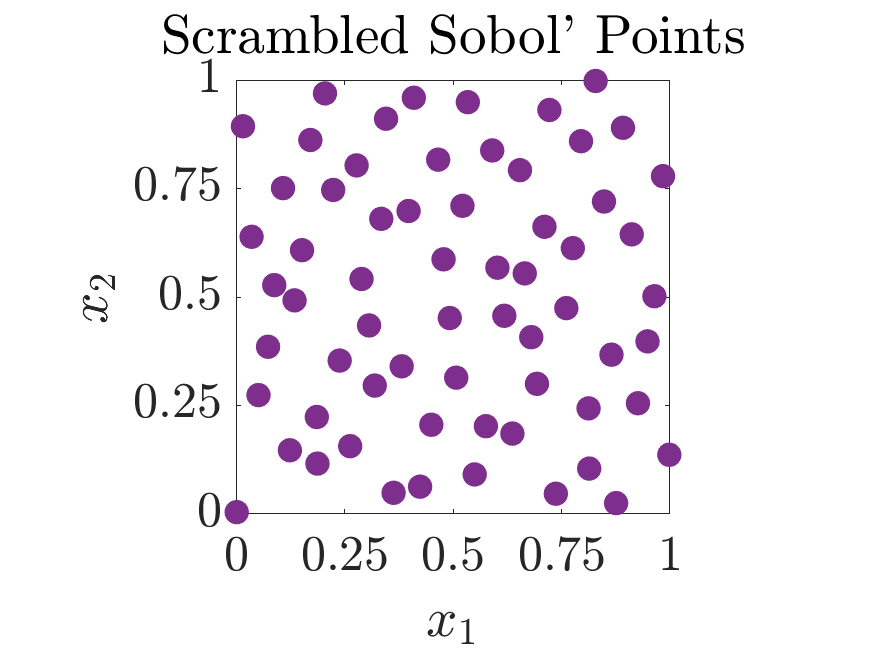
\includegraphics[width=0.8\linewidth]{SSobolPoints}
	\caption{Example of a scrambled Sobol node set  in $d=2$ \label{sobolfig} }
\end{figure}


\Section{Walsh Kernels}

Walsh kernels are product kernels based on the Walsh functions. We introduce the necessary concepts in this section.

\Subsection{Walsh functions}
Like Fourier transform used with Lattice points (Section \ref{sec:shift_invar_kern}), Hadamard-Walsh transform used for the nets, which we will call simply Walsh transform. Walsh transform  is defined using Walsh functions. Define $\naturals:=\lbrace1,2,\dots \rbrace$ and $\naturals_0 : \lbrace0,1,2,\dots \rbrace$.
The one-dimensional Walsh functions in base $b$ are defined as
\begin{align}
\label{eqn:walsh_func}
\textup{wal}_{b,h}(x) := e^{2\pi i (x_1 h_0 + x_2 h_1 + \dots + x_n h_{n-1})/b} 
=
e^{2\pi i [\vec{h}]_n^T[\vec {x}]_n/b}
\end{align}
for $x \in [0,1)$ and $h \in \naturals_0$ and the unique base $b$ expansions 
$x = \sum_{i \ge 1} x_i b^{-i} = (0.x_1 x_2 \dots)_b$,
and
$h = \sum_{i \ge 1} h_i b^{-i} = (0.h_1 h_2 \dots)_b, [\vec{h}] =  (h_1,\dots h_n)^T$,
with $n$ at least as large as the number of digits to represent $x$ or $h$.
Multivariate Walsh functions are defined as the product of the one-dimensional Walsh functions,
\begin{align*}
\textup{wal}_{b,\vh} (\vx) := \prod_{j=1}^s \textup{wal}_{b,h_j} (x_j
)
\end{align*}
As we can see in \eqref{eqn:walsh_func}, the Walsh functions only take the values in $\{1, -1\}$, i.e., $\textup{wal}_{b,\vk} : [0,1] \to {\{-1, 1\}} , \; \vk \in \naturals_0$. Walsh functions form an orthonormal basis of Hilbert space $L^2[0,1]]$,
\begin{align*}
\int_{[0,1]}
\textup{wal}_{b,\vk} (\vx) \textup{wal}_{b,\vm}(\vx) \dx = \delta_{\vk,\vm}
\end{align*}
Digital nets are designed to integrate the Walsh functions without error.
Thus our Bayesian cubature algorithm could integrate linear combinations of its ideal integrands without error. Functions that are well approximated by such linear combinations are then integrated with small errors.

\Subsection{Walsh kernels}
Consider the kernels of the form \cite{Nuyens2013}
\begin{align}
\label{eqn:walsh_kernel}
C_{\vtheta}(\vx, \vt) = 1 + \theta \omega_{r} (\vx \ominus \vt)
\end{align}
where $\ominus$ is bitwise subtraction,
\begin{align*}
\omega_r(x) = \sum_{h=1}^\infty 
\frac{\textup{wal}_{b,h}(x) }{b^{qr \lfloor \log_b h \rfloor}}
\end{align*}
where $r$ is kernel order, $\frac 1p + \frac 1q = 1$ are H\"older inequality coefficients. Explicit expression available for $\omega_{r}$ \cite{Nuyens2013} in case of $b=2$, order $r=1$, and Hilbert space setup $p=q=2$,
\begin{align}
\omega_1(\vx) &= \sum_{h=1}^\infty 
\frac{\textup{wal}_{b,h}(x) }{b^{2 \lfloor \log_b h \rfloor}} = 6\left( \frac 16 - 2^{\lfloor \log_2 \vx\rfloor -1 }\right).
\end{align}

\begin{figure}
	\centering
	\includegraphics[width=0.9\linewidth]{"figures/walsh_kernel dim_1"}
	\caption[Walsh kernel]{Walsh kernel of order $r=1$ in dimension $d=1$. This figure can be reproduced using \code{plot\_walsh\_kernel.m}}
	\label{fig:walshkernel-dim1}
\end{figure}
The \figref{fig:walshkernel-dim1} shows $r=1$ order Walsh kernel in the interval $[0,1]$. Unlike the shift-invariant kernels used with Lattice nodes, low order Walsh kernels are not very smooth but only piecewise constant. Smaller $\eta$ implies lesser variation in the amplitude of the kernel. Also the Walsh kernels are shift invariant but not periodic.

\Subsection{Walsh transform}
% \JRNote{add subsection for walsh transform, define and explain.}
The Walsh-Hadamard transform (WHT) is a generalized class of discrete Fourier transform (DFT) that was used with Lattice nodes, and is much simpler to compute. The Walsh-Hadamard transform matrices comprises of only $\{1, -1\}$ values, so the computation usually involves only additions and subtractions. Hence, the WHT is also sometimes called the integer transform. In comparison DFT uses complex exponential functions and the computation involves complex, non-integer multiplications. 

The Walsh-Hadamard transforms are $2^m \times 2^m$ Walsh-Hadamard matrices, which are constructed recursively, starting with $H_0 = 1$,
\begin{align}
\nonumber
\arraycolsep=1.4pt\def\arraystretch{0.9}
H(1) &=
\begin{pmatrix}
1 & 1 \\ 1 & -1
\end{pmatrix}, \\
\nonumber
H(2^1) &= 
\begin{pmatrix}
1 & 1 & 1 & 1 \\ 
1 & -1 & 1 & -1 \\
1 & 1 & -1 & -1 \\ 
1 & -1 & -1 & 1 \\
\end{pmatrix}, \\
\nonumber
\hdots
\\
\label{eqn:hadamard_matrix}
H(2^m) &= 
\begin{pmatrix}
H(2^{m-1}) & H(2^{m-1}) \\ H(2^{m-1}) & -H(2^{m-1})
\end{pmatrix} = H(1) \bigotimes H(2^{m-1})
\end{align}
where $\bigotimes$ is Kronecker product. Alternatively for $b=2$, these matrices can be  directly obtained by,
\begin{align*}
H(2^m) = \bigg(\exp(\pi \sqrt{-1} [\vec{i}]_m^T[\vec {j}]_m) \bigg)_{i,j=0}^{n-1}  
= \bigg((-1)^{([\vec{i}]_m^T[\vec {j}]_m)} \bigg)_{i,j=0}^{n-1}  
\end{align*}
where the notation $[\vec{i}]_m^T[\vec {j}]_m$ indicates bitwise dot product. 

\iffalse
An example of Walsh matrix of length $n=8$ is given in Table \ref{tab:hadamard_matrix}. 
\begin{table} % 
% \centering
\arraycolsep=1pt\def\arraystretch{0.8}
\[
%\arraycolsep=1.4pt\def\arraystretch{0.9}
\begin{array}{c|@{\quad}r@{\quad}r@{\quad}r@{\quad}r@{\quad}r@{\quad}r@{\quad}r@{\quad}r@{\quad}r}
\hhline{=========}
%\vspace{-1.5ex}
\text{Zero crossings} & \multicolumn{8}{l}{\text{Walsh function values}} \\
\hline
0&	1&  1&  1&  1&  1&  1&  1&  1 \\
4&	1& -1& -1&  1&  1& -1& -1&  1 \\
6&	1& -1&  1& -1& -1&  1& -1&  1 \\
2&	1&  1& -1& -1& -1& -1&  1&  1 \\
3&	1&  1& -1& -1&  1&  1& -1& -1 \\
7&	1& -1&  1& -1&  1& -1&  1& -1 \\
5&	1& -1& -1&  1& -1&  1&  1& -1 \\
1&	1&  1&  1&  1& -1& -1& -1& -1
\end{array}
\]
\vspace{-5ex}
\caption{Walsh transform matrix of for $n=8$, in Hadamard order  \label{tab:hadamard_matrix}}	   
\end{table}
\fi

\Subsection{Fast transform}
We can easily show the Walsh-Hadamard matrices satisfy the assumptions of fast-transform \eqref{fastcompAssump} $\mV^H$. Its important to note that the columns/rows of Walsh-Hadamard matrices are mutually orthogonal. Assumption \eqref{fastcompAssumpB} follows automatically by the fact that the Walsh-Hadamard matrices can be constructed analytically. Assumption \eqref{fastcompAssumpA} can also be verified as the first row/column are one vectors. Finally, assumption \eqref{fastcompAssumpC} is satisfied due to the fact that fast Walsh transform can be computed in $\Order({n \log n})$ operations using fast Walsh-Hadamard transform. Thus the Walsh-Hadamard is a fast transform as per the \eqref{fastcompAssump},
\begin{align}
\label{eqn:hadamard_fwht}
\mV^{2^m} = H_{2^m}
\end{align}

% \JRNote{prove eigenvalues for Sobol case}

We have implemented a fast adaptive Bayesian cubature algorithm using the kernel \eqref{eqn:walsh_kernel} with $r=1$ and Sobol points \cite{BraFox88} in MATLAB as part of the Guaranteed Adaptive Integration Library (GAIL) \cite{ChoEtal17b} as \allowbreak \code{cubBayesNet\_g}. The Sobol points used in this algorithm are generated using Matlab's builtin function \code{sobolset} and scrambled using Matlab function \code{scramble} \cite{HonHic00a}. The fast Walsh-Hadamard transform \eqref{eqn:hadamard_fwht} is computed using Matlab's builtin function \code{fwht} with `hadamard' ordering.

\Subsection{Extensible Sobol points}
Similar to the extensible Lattice points, Sobol points could be extended to improve the integration accuracy till the required error tolerance is met. Extensible Sobol point-set can be combined with Hadamard matrices as demonstrated here. Using the same notations as in \secref{sec:iter_fft},
\begin{align*}
\widetilde{\vb}^{(2)} &= H_{2^m} {\vb}^{(2)}, \\
& = \begin{pmatrix}
H_{2^{m-1}} & H_{2^{m-1}} \\ H_{2^{m-1}} & -H_{2^{m-1}}
\end{pmatrix} 
\begin{pmatrix}
\vb^{(1)} \\ \vb^{(2)}
\end{pmatrix}, \qquad \text{by \eqref{eqn:hadamard_matrix}} \\
&= 
\begin{pmatrix}
H_{2^{m-1}} \vb^{(1)} + H_{2^{m-1}} \vb^{(2)} \\ 
H_{2^{m-1}} \vb^{(1)} - H_{2^{m-1}} \vb^{(2)}
\end{pmatrix}.
\end{align*}
As before with the Lattice nodes, the computational cost to compute $\mV^{(2n)H} \vb$ is then
twice the cost of computing $\mV^{(n)H} \vb^{(1)}$ plus $2n$ additions. An inductive argument shows that $\mV^{(n)H}b$ requires only $\Order(n \log(n))$ operations. Usually the multiplications in $\mV^{(n)H} \vb^{(1)}$ are multiplications by $-1$ which are simply accomplished using negations, requiring no multiplications at all.


\Subsection{Higher order nets}
Higher order digital nets are a modified $(t,m,d)$-nets, introduced in \cite{Dic08a} can be used to numerically integrate smoother functions which are not necessarily periodic, but have square integrable mixed partial derivatives of order $\alpha$, at a rate of $\Order(N^{-\alpha})$ multiplied by a power of a $\log N$ factor using rules corresponding to the modified $(t,m, d)$-nets.
We want to emphasizes that quasi-Monte Carlo rules based on these point sets can achieve convergence rates faster than $\Order(N^{-1})$.

Higher order digital nets are constructed using matrix-vector multiplications over finite
fields. Bayesian cubatures using higher order digital nets are the topic for future research.


\Section{Summary}

We summarize the results of this Chapter as a proposition,
\begin{prop}
	Any symmetric, positive definite, shift-invariant covariance kernel of the form \eqref{eq:shInv} scaled to satisfy \eqref{addAssump}, when matched with digital net data-sites, must satisfy assumptions \eqref{fastcompAssump}.  The \emph{fast Walsh-Hadamard transform} (FWHT) can be used to expedite the estimates of $\vtheta$ in \eqref{thetaSimple} and the credible interval widths \eqref{fastStoppingCriterions} in $\Order(n \log(n))$ operations. The cubature, $\hmu$, is just the sample mean.
\end{prop}



\clearpage







\Chapter{Numerical Implementation} 
\label{sec:NumExp}

\Section{Overcoming the Cancellation error}
\label{sec:overcome_cancel_error}

For the kernels used in our computation it may happen that $n/\lambda_1$ is close to $1$.  Thus, the term $1-n/\lambda_1$, which appears in the credible interval widths, $\err_{\MLE}$, $\err_{\textup{full}}$, and $\err_{\textup{GCV}}$, may suffer from cancellation error.  We can avoid this cancellation error by modifying how we compute the Gram matrix and its eigenvalues.

Define a new function $\rC : = C -1$, and its associated Gram matrix $\rmC = \mC - \vone \vone^T$.   Note that $\rC$ inherits the shift-invariant properties of $C$.  Since $\vone$ is the first eigenvector of $\mC$ it follows that the eigenvalues of $\rmC$ are $\rlambda_1 = \lambda_1 - n, \lambda_2, \ldots, \lambda_n$.  Moreover,
\begin{equation*}
1 - \frac{n}{\lambda_1}  = \frac{\lambda_1 - n}{\lambda_1} = \frac{\rlambda_1}{\rlambda_1 +n},
\end{equation*}
where now the right hand side is free of cancellation error.

We show how to compute $\rC$ without introducing round-off error.  The covariance functions that we use are of product form, namely,
\begin{equation*}
C(\vt, \vx) = \prod_{\ell=1}^d \left[1 + \rC_\ell(t_\ell,x_\ell) \right], \qquad  \rC_\ell:[0,1]^2 \to \reals.
\end{equation*}
Direct computation of $\rC (\vt,\vx) = C(\vt,\vx) -1$ introduces cancellation error if the $ \rC_\ell$ are small.  So, we employ the iteration
\begin{align*}
\rC^{(1)} &= \rC_1(t_1,x_1),  \\
\rC^{(\ell)} &  = \rC^{(\ell-1)}[1 + \rC_\ell(t_\ell,x_\ell)] + \rC_\ell(t_\ell,x_\ell),  \hspace{1cm} \ell = 2, \ldots, d, \\
\rC(\vt,\vx)  & = \rC^{(d)}.
\end{align*}
In this way, the Gram matrix $\rmC$, whose $i,j$-element is $\rC(\vx_i,\vx_j)$ can be constructed with minimal round-off error.

Computing the eigenvalues of $\rmC$ via the procedure given in \eqref{eqn:fast_transform_to_eigvalues} yields $\rlambda_1 = \lambda_1 - n, \lambda_2, \ldots, \lambda_n$. The estimates of $\vtheta$ are computed in terms of the eigenvalues of $\rmC$, so \eqref{eqn_MLE_loss_func_optimized_2} and \eqref{thetaGCV} become
\begin{subequations}
	\label{thetaSimple}
	\begin{align}
	\vtheta_\MLE
	&= 
	\argmin_{\vtheta}
	\left[
	\log\left(
	\sum_{i=2}^n \frac{\abs{\widetilde{y}_i}^2}{\lambda_i}
	\right) 
	%\label{thetaMLEsimple}
	+ 
	\frac{1}{n}\sum_{i=1}^n \log(\lambda_i)
	\right], \\
	\vtheta_{\GCV} 
	&= \argmin_\vtheta \left[ \log \left ( \sum_{i=2}^n \frac{\abs{\widetilde{y}_i}^2}{\lambda_i^2} 
	\right)  -2\log\left( \sum_{i=1}^n \frac{1}{\lambda_i} \right)
	\right],
	\end{align}
\end{subequations}
where $\lambda_1 = n + \rlambda_1$.  The widths of the credible intervals in \eqref{eq:errMLEAllAsump}, \eqref{FJH:eq:errFullSimple}, and   \eqref{errGCVSimple} become
\begin{subequations}
	\label{fastStoppingCriterions}
	\begin{align}
	\err_\MLE  &
	=
	\frac{2.58}{n}\sqrt{
		\frac{\rlambda_1}{\lambda_1}
		\sum_{i=2}^{n} \frac{\abs{\widetilde{y}_i}^2}{\lambda_i}  
	}, 
	\\
	\err_{\textup{full}} 
	& = \frac{t_{n_j-1,0.995}}{n} \sqrt{
		\frac{\rlambda_1}{n-1} \sum_{i=2}^n \frac{\abs{\widetilde{y}_i}^2}{\lambda_i}
	}, \\
	\err_{\textup{GCV}} & =
	\frac{2.58}{n}\sqrt{	\frac{\rlambda_1}{\lambda_1} \sum_{i=2}^n \frac{\abs{\widetilde{y}_i}^2}{\lambda_i^2}  \left [ \frac 1n \sum_{i=1}^n \frac{1}{\lambda_i} \right]^{-1}} .
	\end{align}
\end{subequations}
Since $\rlambda_1 = \lambda_1 - n$ and $\lambda_1 \sim n$ it follows $\rlambda_1/\lambda_1 \approx \rlambda_1/(n-1)$ and is small for  large $n$.  Moreover, the credible intervals via empirical Bayes and full Bayes are similar, since $t_{n_j-1,0.995}$ is approximately $2.58$. 

\iffalse 
Whereas to compare $\err_\GCV$, need little more insight due to the term $\lambda_i^2$ in the denominator. Rewriting it:
\begin{align*}
\err_\GCV^2 & =
\frac{2.58^2}{n^2}	\frac{\rlambda_1}{n + \rlambda_1} \frac{ \sum_{i=2}^n \left( \frac{\abs{\widetilde{y}_i}^2}{\lambda_i} \frac{1}{\lambda_i} \right)}{ \frac 1n \sum_{i=1}^n \frac{1}{\lambda_i} } 
\end{align*}
If the eigenvalues are ordered with $n$ then,
\[
\frac{1}{\lambda_n} \geq \frac{1}{\lambda_{n-1}} ... \geq \frac{1}{\lambda_1} 
\]
Note that we assumed the kernel Gram matrix is positive definite, so all the eigen values are positive
\begin{align*}
\frac{ \sum_{i=2}^n \left( \frac{\abs{\widetilde{y}_i}^2}{\lambda_i} \frac{1}{\lambda_i} \right)}{ \frac 1n \sum_{i=1}^n \frac{1}{\lambda_i} } 
\leq 
\frac{ \frac{1}{\lambda_n} \sum_{i=2}^n \frac{\abs{\widetilde{y}_i}^2}{\lambda_i}  }{ \frac 1n n \frac{1}{\lambda_1} } 
\leq 
\frac{\lambda_1}{\lambda_n} \sum_{i=2}^n  \frac{\abs{\widetilde{y}_i}^2}{\lambda_i}  
\end{align*}
Thus we can write
\begin{align*}
\err^2_\GCV \leq \frac{\lambda_1}{\lambda_n} \err^2_\MLE
\end{align*}
This shows the $\err_\GCV$ is more aggressive stopping criterion than $\err_\MLE$. If the chosen kernel is very smooth then eigen values decay very quickly with increasing $n$. 
\fi





\Section{Kernel parameters search}


\JRNote{Explain the transformation used to make the search range positive, > 0 , etc.}

The various parameters introduced and used by our algorithms so far needs to be optimally chosen. We have not discussed how that will be done. One could use bounded minima search if the search interval is known, like the \code{fminbnd} provided by Matlab.  Most of the time time, we may not know that. So the natural choice is to use unbounded search like the \code{fminsearch} provided by Matlab. But the parameter needs to be sometimes positive only or greater than value. We use some simple domain transformations to achieve such constraints.

\Subsection{Positive kernel shape parameter}
The following function map is used to have the shape parameter values positive
% We need to have $\eta > 0$ and $ 0 < b < 1$ while searching for the optimum value, so we use the following transformations
\begin{align*}
\eta: & \quad h(t) = e^{t}, & h:(-\infty, \infty) \to (0, \infty)
\end{align*}




\Subsection{Kernel order $0 < b < 1$}
The following map is used to have the kernel order value in the range
\begin{align*}
b: & \quad g(t) = \frac{1}{1 + e^{-t}}, & g:(-\infty, \infty) \to (0, 1)
\end{align*}


\clearpage



\Chapter{Numerical Results and Observations} 

\JRNote{use uniformly randomly chosen $\varepsilon$ instead 4 fixed}

Bayesian cubature algorithms developed in this work are demonstrated using widely used integration examples.
Three integrals were evaluated using both the algorithms \code{cubBayesLattice\_g} and \code{cubBayesNet\_g}. The first example shows evaluating a multivariate normal probability given the intervals. The second example shows integrating the Keister's function, and the final example shows computing an Asian arithmetic option pricing.  

% \Section{Test Results and Observations for \code{cubBayesLattice\_g}}
\Section{Testing Methodology}
\label{sec:numerical_experiments_cubBayesLattice}

Four different error tolerances, $\varepsilon$,  were set for each example, with the tolerances chosen depending on the difficulty of the problem.  The nodes used in \allowbreak \code{cubBayesLattice\_g} were the randomly shifted lattice rules supplied by GAIL.  
Where as the nodes used in \code{cubBayesNet\_g} were the randomly scrambled Sobol rules supplied by Matlab's Sobol sequence generator. 

For each integral,  each tolerance, and each of our stopping criteria---empirical Bayes, full Bayes, and generalized cross-validation---our algorithm is run  $100$ times.  For each test, the execution time is plotted against $\abs{\mu - \hmu}/\varepsilon$.  We expect $\abs{\mu - \hmu}/\varepsilon$ to be no greater than one, but hope that it is not too much smaller than one, which would indicate a stopping criterion that is too conservative.
%Unlike the examples in previous \secref{sec:numerical_experiments_cubBayesLattice}, periodization variable transform is not required.

Periodization variable transforms are used in the examples with \allowbreak \code{cubBayesLattice\_g} as the algorithms assumes the integrands to be periodic in $[0,1]^d$. But the \allowbreak \code{cubBayesNet\_g} does not need this additional requirement, So the integrands are used directly.

% \Section{Test Results and Observations for \code{cubBayesNet\_g}}
% \label{sec:numerical_experiments_cubBayesNet}

%Similar to the previous examples, we used four different error tolerances, $\varepsilon$,  set for each example, with the tolerances chosen depending on the difficulty of the problem.  
%For each integral,  each tolerance, and each of our stopping criteria---empirical Bayes, full Bayes, and generalized cross-validation---our algorithm is run  $100$ times.  For each test, the execution time is plotted against $\abs{\mu - \hmu}/\varepsilon$.  
% We expect $\abs{\mu - \hmu}/\varepsilon$ to be no greater than one, but hope that it is not too much smaller than one, which would indicate a stopping criterion that is too conservative. 

\Section{Multivariate Normal Probability}

This example was already introduced in Section \ref{MVN_example}, where we used the Mat\'ern covariance kernel.  We reuse $ f_{\textup{Genz}}$ \eqref{eqn:fGenzdef} and apply periodization transform when required.

\Subsection{Using \code{cubBayesLattice\_g}}
As required by the algorithm, we apply Sidi's $C^2$  periodization to $ f_{\textup{Genz}}$ \eqref{eqn:fGenzdef}, and chose $d=3$ and $r=2$. The simulation results for this example function are summarized in Figures \ref{fig:mvn-guaranteed-MLE}, \ref{fig:mvn-guaranteed-FB}, and \ref{fig:mvn-guaranteed-GCV}.  In all cases the Bayesian cubature returns an approximation within the prescribed error tolerance. We used the same setting as before with generic slow Bayesian cubature in \secref{MVN_example} for comparision. For error threshold $\varepsilon=10^{-5}$ with empirical stopping criterion, our fast algorithm takes 0.001 seconds as shown in \figref{fig:mvn-guaranteed-MLE} whereas the basic algorithm takes 30 seconds as shown in \figref{fig:MVN_Metern_d2b2}. 
Amongst the three stopping criteria, GCV achieved the results faster than others. 
One can also observe from the figures, the credible intervals are wider, causing the true error much smaller than requested.
This could be due to the periodization transformed $f_\textup{Genz}$ is smoother than the $r=2$ kernel could approximate. Using a kernel of matching smoothness could produce right credible intervals.

\begin{figure}
	\centering
	%d=3 problem transformed into d=2
	\includegraphics[width=0.95\linewidth]{"Lattice/Lattice_MVN_guaranteed_time_MLE_C2sin_d2_r2_2019-Jun-27"}
	\caption[Lattice: MVN guaranteed: MLE]{\code{cubBayesLattice\_g}: Multivariate normal probability example using the empirical Bayes stopping criterion.}
	\label{fig:mvn-guaranteed-MLE}
\end{figure}
\begin{figure}
	\centering
	\includegraphics[width=0.95\linewidth]{"Lattice/Lattice_MVN_guaranteed_time_full_C2sin_d2_r2_2019-Jun-27"}
	\caption[Lattice: MVN guaranteed: Full Bayes]{\code{cubBayesLattice\_g}: Multivariate normal probability example using the full Bayes stopping criterion.}
	\label{fig:mvn-guaranteed-FB}
\end{figure}
\begin{figure}
	\centering
	\includegraphics[width=0.95\linewidth]{"Lattice/Lattice_MVN_guaranteed_time_GCV_C2sin_d2_r2_2019-Jun-27"}
	\caption[Lattice: MVN guaranteed: GCV]{\code{cubBayesLattice\_g}: Multivariate normal probability example using the GCV stopping criterion.}
	\label{fig:mvn-guaranteed-GCV}
\end{figure}





\Subsection{Using \code{cubBayesNet\_g}}
Here we use $ f_{\textup{Genz}}$ \eqref{eqn:fGenzdef} without any periodization, and chose $d=3$ and $r=1$. The simulation results for this example function are summarized in Figures \ref{fig:Sobol-mvn-guaranteed-MLE}, \ref{fig:Sobol-mvn-guaranteed-FB}, and \ref{fig:Sobol-mvn-guaranteed-GCV}.  In all cases the {\code{cubBayesNet\_g} returns an approximation within the prescribed error tolerance. We used the same setting as before with generic slow Bayesian cubature in \secref{MVN_example} for comparision. For error threshold $\varepsilon=10^{-5}$ with empirical stopping criterion, our fast algorithm takes about 2 seconds as shown in \figref{fig:mvn-guaranteed-MLE} whereas the basic algorithm takes 30 seconds as shown in \figref{fig:MVN_Metern_d2b2}. 
{\code{cubBayesNet\_g} uses fast Walsh transform which is slower in Matlab due to the way it was implemented. This is reason it takes more time than the {\code{cubBayesLattice\_g}. 
But comparing the number of samples, $n$, used for integration provides more insight which directly relates to the alogrithm's computational cost. The {\code{cubBayesLattice\_g} used $n=16384$ samples whereas {\code{cubBayesNet\_g} used $n=32768$ samples even with $r=1$ order kernel.

Amongst the three stopping criteria, GCV achieved the results faster than others. 
One can also observe from the figures, the credible intervals are narrower than we observed in \figref{fig:mvn-guaranteed-MLE}.
This shows {\code{cubBayesNet\_g} with $r=1$ kernel more accurately approximates the integrand.

\begin{figure}
\centering
%d=3 problem transformed into d=2
\includegraphics[width=0.95\linewidth]{"Sobol/Sobol_MVN_guaranteed_time_MLE__d2_r1_2019-Jun-17"}
\caption[Sobol: MVN guaranteed: MLE]{\code{cubBayesNet\_g}: Multivariate normal probability example with empirical Bayes stopping criterion.}
\label{fig:Sobol-mvn-guaranteed-MLE}
\end{figure}
\begin{figure}
\centering
%d=3 problem transformed into d=2
\includegraphics[width=0.95\linewidth]{"Sobol/Sobol_MVN_guaranteed_time_full__d2_r1_2019-Jun-17"}
\caption[Sobol: MVN guaranteed: Full Bayes]{\code{cubBayesNet\_g}: Multivariate normal probability example with the full-Bayes stopping criterion.}
\label{fig:Sobol-mvn-guaranteed-FB}
\end{figure}
\begin{figure}
\centering
%d=3 problem transformed into d=2
\includegraphics[width=0.95\linewidth]{"Sobol/Sobol_MVN_guaranteed_time_GCV__d2_r1_2019-Jun-17"}
\caption[Sobol: MVN guaranteed: GCV]{\code{cubBayesNet\_g}: Multivariate normal probability example with the GCV stopping criterion.}
\label{fig:Sobol-mvn-guaranteed-GCV}
\end{figure}






\Section{Keister's Example}

This multidimensional integral function comes from \cite{Kei96} and is inspired by a physics application:
\begin{align}
\label{eqn:keister_integral}
\mu & =  \int_{\reals^d} \cos(\norm{ \vt}) \exp(-\norm{ \vt }^2) \, \dvt \\
\nonumber
%&  = 
%\int_{\reals^d} \cos(a\norm{ \vt}) \exp(-a^2\norm{ \vt }^2)  a^d \, \dvt \\
& = \int_{[0,1]^d} f_{\textup{Keister}}(\vx) \, \dvx,\\
\intertext{where }
\nonumber
f_\textup{Keister}(\vx) &= \pi^{d/2} \cos\left(\norm{ \Phi^{-1}(\vx)/2}\right)  ,
\end{align}
and again $\Phi$ is the standard normal distribution.
%\begin{figure}
%	\captionsetup[subfigure]{labelformat=empty}
%	\begin{subfigure}[h]{0.48\linewidth}
%		\includegraphics[width=1.1\linewidth]{Keister_wholeR_1D}
%	\end{subfigure}
%	\begin{subfigure}[h]{0.48\linewidth}
%		\includegraphics[width=1.1\linewidth]{Keister_cube_1D}
%	\end{subfigure}
%	\caption{Keister function in d=2 and its transformed version in $[0,1]^2$ with various values of $a$.}
%	\label{fig:keister}
%\end{figure}
The true value of $\mu$ can be calculated iteratively in terms of a quadrature as follows:  
\begin{equation*}
\mu = \frac{2 \pi^{d/2} I_c(d)}{\Gamma(d/2)}, \quad d=1,2, \ldots
\end{equation*}
where $\Gamma$ denotes the gamma function, and
\begin{align*}
I_c(1) &= \frac{\sqrt{\pi}}{2 \exp(1/4)}, 
\\
I_s(1) &= \int_{x=0}^\infty \exp(-\vx^T\vx)\sin(\vx) \, \dvx 
\\
& =  0.4244363835020225,
\\
I_c(2) &= \frac{1-I_s(1)}{2}, \qquad
I_s(2) = \frac{I_c(1)}{2}
\\
I_c(j) &= \frac{(j-2)I_c(j-2)-I_s(j-1)}{2},
\qquad j =3,4,\ldots
\\
I_s(j) &= \frac{(j-2)I_s(j-2)-I_c(j-1)}{2},
\qquad j =3,4,\ldots.
% ref: https://www.mathworks.com/help/matlab/ref/gamma.html
\end{align*}

\Subsection{Using \code{cubBayesLattice\_g}}
\label{sec:cubBayesLattice_keister_example}
\JRNote{Discuss the big gap between 1e-5 and 1e-4}
\begin{figure}
	\centering
	\includegraphics[width=0.95\linewidth]{"Lattice/Lattice_Keister_guaranteed_time_MLE_C1sin_d4_r2_2019-Jun-27"}
	\caption[Lattice: Keister guaranteed: MLE]{\code{cubBayesLattice\_g}: Keister example using the empirical Bayes stopping criterion.}
	\label{fig:keister-guaranteed-MLE}
\end{figure}
\begin{figure}
	\centering
	\includegraphics[width=0.95\linewidth]{"Lattice/Lattice_Keister_guaranteed_time_full_C1sin_d4_r2_2019-Jun-27"}
	\caption[Lattice: Keister guaranteed: Full Bayes]{\code{cubBayesLattice\_g}: Keister example using the full Bayes stopping criterion.}
	\label{fig:keister-guaranteed-FB}
\end{figure}
\begin{figure}
	\centering
	\includegraphics[width=0.95\linewidth]{"Lattice/Lattice_Keister_guaranteed_time_GCV_C1sin_d4_r2_2019-Jun-27"}
	\caption[Lattice: Keister guaranteed: GCV]{\code{cubBayesLattice\_g}: Keister example using the GCV stopping criterion.}
	\label{fig:keister-guaranteed-GCV}
\end{figure}
Figures \ref{fig:keister-guaranteed-MLE}, \ref{fig:keister-guaranteed-FB} and \ref{fig:keister-guaranteed-GCV} summarize the numerical tests for this integral.  We used the Sidi's $C^1$ periodization, dimension $d=4$, and $r=2$. 
As we can see the GCV stopping criterion achieved the results faster than the others similar to the multivariate normal case.

\Subsection{Using \code{cubBayesNet\_g}}
Figures \ref{fig:Sobol-keister-guaranteed-MLE}, \ref{fig:Sobol-keister-guaranteed-FB} and \ref{fig:Sobol-keister-guaranteed-GCV} summarize the numerical tests for this case. We used  dimension $d=4$, and $r=1$.  No periodization transform was used as the integrand need not be periodic. 
In this example, we use $r=1$ order kernel where as in \secref{sec:cubBayesLattice_keister_example}, $r=2$ kernel was used, which necessitates
the \code{cubBayesNet\_g} to use more samples for integration.
As we can see the GCV stopping criterion achieved the results faster than the others similar to the multivariate normal case.

\begin{figure}
	\centering
	\includegraphics[width=0.95\linewidth]{"Sobol/Sobol_Keister_guaranteed_time_MLE__d4_r1_2019-Jun-17"}
	\caption[Sobol: Keister guaranteed: MLE]{\code{cubBayesNet\_g}: Keister example using the empirical Bayes stopping criterion.}
	\label{fig:Sobol-keister-guaranteed-MLE}
\end{figure}
\begin{figure}
	\centering
	\includegraphics[width=0.95\linewidth]{"Sobol/Sobol_Keister_guaranteed_time_full__d4_r1_2019-Jun-17"}
	\caption[Sobol: Keister guaranteed: Full Bayes]{\code{cubBayesNet\_g}: Keister example using the full-Bayes stopping criterion.}
	\label{fig:Sobol-keister-guaranteed-FB}
\end{figure}
\begin{figure}
	\centering
	\includegraphics[width=0.95\linewidth]{"Sobol/Sobol_Keister_guaranteed_time_GCV__d4_r1_2019-Jun-17"}
	\caption[Sobol: Keister guaranteed: GCV]{\code{cubBayesNet\_g}: Keister example using the GCV stopping criterion.}
	\label{fig:Sobol-keister-guaranteed-GCV}
\end{figure}







\Section{Option Pricing}

The price of financial derivatives can often be modeled by high dimensional integrals. If the underlying asset is described in terms of a discretized geometric Brownian motion, then the fair price of the option is:
\begin{equation*}
\mu = \int_{\reals^d} \text{payoff}(\vz) \frac{\exp(\frac 12 \vz^T\mSigma^{-1}\vz)}{\sqrt{(2\pi)^d \det(\mSigma)}} \, \dvz = \int_{[0,1]^d} f(\vx) \, \dvx,
\end{equation*} 
where {payoff($\cdot$)} defines the discounted payoff of the option,
\begin{align*}
\mSigma &= (T/d) \bigl(\min(j,k) \bigr)_{j,k=1}^d = \mL \mL^T,\\
f(\vx) &= \text{payoff} \left(\mL 
\begin{pmatrix}
\Phi^{-1}(x_1) \\ \vdots \\ \Phi^{-1}(x_d)
\end{pmatrix} \right).
\end{align*}
The Asian arithmetic mean call option has a payoff of the form
\begin{align*}
\text{payoff}(\vz) &= \max\left( \frac 1d  \sum_{j=1}^d S_j(\vz) - K, 0 \right) \me^{-r T}, \\
S_j(\vz) &= S_0 \exp\bigl((r-\sigma^2/2)jT/d + \sigma \sqrt{T/d} z_j \bigr).
\end{align*}
Here, $T$ denotes the time to maturity of the option, $d$ the number of time steps, $S_0$ the initial price of the stock, $r$ the interest rate, $\sigma$ the volatility, and $K$ the strike price.  

\Subsection{Using \code{cubBayesLattice\_g}}
The Figures \ref{fig:optprice-guaranteed-MLE}, \ref{fig:optprice-guaranteed-FB} and 
\ref{fig:optprice-guaranteed-GCV} summarize the numerical results for this example using
$
T = 1/4, \ \ d = 13, \ \ S_0 = 100, \ \ r =  0.05, \ \ \sigma = 0.5, \ \ K = 100.
$
Moreover, $\mL$ is chosen to be the matrix of eigenvectors of $\mSigma$ times the square root of the diagonal matrix of eigenvalues of $\mSigma$.
Because the integrand has a kink caused by the $\max$ function, it does not help to use a periodizing transform that is very smooth.  We choose the baker's transform \eqref{eq:bakerTrans} and $r = 1$.


\label{sec:cubBayesLattice_option_pricing_example}
\begin{figure}
	\centering
	\includegraphics[width=0.95\linewidth]{"Lattice/Lattice_optPrice_guaranteed_time_MLE_Baker_d12_r1_2019-Jul-9"}
	\caption[Lattice: Option pricing guaranteed: MLE]{\code{cubBayesLattice\_g}: Option pricing using the empirical Bayes stopping criterion.}
	\label{fig:optprice-guaranteed-MLE}
\end{figure}
\begin{figure}
	\centering
	\includegraphics[width=0.95\linewidth]{"Lattice/Lattice_optPrice_guaranteed_time_full_Baker_d12_r1_2019-Jul-9"}
	\caption[Lattice: Option pricing guaranteed: Full Bayes]{\code{cubBayesLattice\_g}: Option pricing using the full Bayes stopping criterion.}
	\label{fig:optprice-guaranteed-FB}
\end{figure}
\begin{figure}
	\centering
	\includegraphics[width=0.95\linewidth]{"Lattice/Lattice_optPrice_guaranteed_time_GCV_Baker_d12_r1_2019-Jul-8"}
	\caption[Lattice: Option pricing guaranteed: GCV]{\code{cubBayesLattice\_g}: Option pricing using the  GCV stopping criterion.} \label{fig:optprice-guaranteed-GCV}
\end{figure}


\Subsection{Using \code{cubBayesNet\_g}}
%\Subsection{Option Pricing}
The Figures \ref{fig:Sobol-optprice-guaranteed-MLE}, \ref{fig:Sobol-optprice-guaranteed-FB} and 
\ref{fig:Sobol-optprice-guaranteed-GCV} summarize the numerical results for the option pricing example using the same values as in \secref{sec:cubBayesLattice_option_pricing_example},
$
T = 1/4, \ \ d = 13, \ \ S_0 = 100, \ \ r =  0.05, \ \ \sigma = 0.5, \ \ K = 100.
$
As mentioned before, this integrand has a kink caused by the $\max$ function, So, \code{cubBayesNet\_g} could be more efficient than \code{cubBayesLattice\_g}, as no periodization transform is required. This can be observed from the number of samples used for intgration to meet the same error threshold. For the error tolerance $\varepsilon=10^{-3}$, the \code{cubBayesLattice\_g} used $n=2^{20}$ samples, whereas the \code{cubBayesNet\_g} used $n=2^{17}$ samples.


\begin{figure}
	\centering
	\includegraphics[width=0.95\linewidth]{"Sobol/Sobol_optPrice_guaranteed_time_MLE__d12_r1_2019-Jun-13"}
	\caption[Sobol: Option pricing guaranteed: MLE]{\code{cubBayesNet\_g}: Option pricing using the empirical Bayes stopping criterion.}
	\label{fig:Sobol-optprice-guaranteed-MLE}
\end{figure}
\begin{figure}
	\centering
	\includegraphics[width=0.95\linewidth]{"Sobol/Sobol_optPrice_guaranteed_time_full__d12_r1_2019-Jun-13"}
	\caption[Sobol: Option pricing guaranteed: Full Bayes]{\code{cubBayesNet\_g}: Option pricing using the full-Bayes stopping criterion.}
	\label{fig:Sobol-optprice-guaranteed-FB}
\end{figure}
\begin{figure}
	\centering
	\includegraphics[width=0.95\linewidth]{"Sobol/Sobol_optPrice_guaranteed_time_GCV__d12_r1_2019-Jun-13"}
	\caption[Sobol: Option pricing guaranteed: GCV]{\code{cubBayesNet\_g}: Option pricing using the GCV stopping criterion.}
	\label{fig:Sobol-optprice-guaranteed-GCV}
\end{figure}




\Section{Discussion}

As shown in Figures \ref{fig:mvn-guaranteed-MLE} to \ref{fig:Sobol-optprice-guaranteed-GCV}, both the algorithms computed integral within user specified threshold most of the times except on a few occasions. This is especially the case with option pricing example due to the complexity and high dimension of the integrand. 
Also notice the \code{cubBayesLattice\_g} algorithm finished within 10seconds of time for Keister and multivariate Normal. For the option pricing it look closer to 70seconds. This is again due to the complexity of the integrand.

Another noticeable aspect from the plots of \code{cubBayesLattice\_g} is how much the error bounds differ from the true error. For option pricing example, the error bound is not as conservative as it is for the multivariate normal and Keister examples. A possible reason is that the latter integrands are significantly smoother than is assumed by our covariance kernel.  This is a matter for further investigation.

% As shown in Figures \ref{fig:Sobol-mvn-guaranteed-MLE} to \ref{fig:Sobol-optprice-guaranteed-GCV}, the \code{cubBayesNet\_g} algorithm computes the integral within user specified threshold most of the times except on a few occasions. This is especially the case with option pricing example due to the complexity and high dimension of the integrand as mentioned in the previous example. 




Most noticeable aspect from the plots of \code{cubBayesNet\_g} is how closer the error bounds are to the true error. 
This shows the \code{cubBayesNet\_g}'s estimation of expected error in the stopping criterion is very accurate. 
Similar to \code{cubBayesLattice\_g}, it missed to meet the given error threshold for the option pricing example, as marked by the hollow stars, for $\varepsilon=10^{-4}$. This is because the complexity of the integrand and the algorithm reached max allowed number of samples $n=2^{20}$.





\Section{Comparison with \code{cubMC\_g}, \code{cubLattice\_g} and \code{cubSobol\_g}}

GAIL library provides variety of numerical integration algorithms based on different theoretical foundation, We would like to compare how our algorithms perform relatively. We consider three GAIL algorithms 1) \code{cubMC\_g} a simple Monte-Carlo method for multi-dimensional integration, 2) \code{cubLattice\_g} a quasi-Monte-Carlo method using Lattice points, and 3) \code{cubSobol\_g} a quasi-Monte-Carlo method using Sobol points.

\Subsection{Keister integral}
The Table~\ref{tab2} summarizes the performance of the methods MC, Lattice, Sobol,
BayesLat, and BayesSob---they refer to the GAIL cubatures, \texttt{cubMC\_g},
\code{cubLattice\_g}, \code{cubSobol\_g},  \code{cubBayesLattice\_g},  \code{cubBayesNet\_g},
respectively for estimating Keister integral defined in \eqref{eqn:keister_integral}.
We conducted two simulations with $d=3,8$. In the case of $d=3$, all five methods succeeded completely meaning the
absolute error is less than given tolerance, i.e., $|\mu - \hat{\mu}| \le
\varepsilon$, where $\hat{\mu}$ is a cubature's approximated value. The
fastest method was \code{cubBayesLattice\_g}.
In the case of $d=8$,   \code{cubSobol\_g} achieved 100\% success rate
and was the fastest. But \code{cubBayesLattice\_g}  was competitive and
had the smallest average absolute error. \code{cubBayesNet\_g} used lowest number of samples in case of $d=8$ but slower than \code{cubSobol\_g}.

\JRNote{avoid Exp notation for 2 decimals}
\begin{table}[ht] % MATLAB Driver: KeisterCubatureExampleBayes.m
	\arrayrulecolor[HTML]{DB5800}
\centering
\caption{Comparison of average performance of cubatures for estimating the integral \eqref{eqn:keister_integral}
for $1000$ independent runs. These results can be conditionally reproduced with the
script, \code{KeisterCubatureExampleBayes.m}, in GAIL. 
\label{tab2}}	   
%\vspace{-2ex}
\begin{tabular}{c}
$
\arraycolsep=1.4pt\def\arraystretch{0.9}
\begin{array}{l@{\quad}r@{\quad}r@{\quad}r@{\quad}r@{\quad}r@{\quad}r}
\hhline{======}
\input{KeisterBayesOut.txt} 
\end{array}
$
\end{tabular}
\end{table}





\Subsection{Multi-variate Normal}
The Table~\ref{tab3} summarizes the performance of the methods MC, Lattice, Sobol,
BayesLat, and BayesSob for estimating the multi-dimensional Normal probability $\bf{X}\sim N(\bf{\mu},\Sigma)$. This experiment demonstrates our algorithm's ability to handle very high-dimensional integral.

We conducted two simulations with different $\Sigma$ and estimation intervals $(\bf{a}, \bf{b})$ but fixed $\mu=0$ and required error threshold $\varepsilon=10^{-3}$. In the first case, all five methods succeeded completely. 
The fastest method was \code{cubBayesLattice\_g} but code{cubBayesNet\_g} used the lowest number of samples.
In the second case also all five methods succeeded,  but \code{cubLattice\_g} was the fastest. 
The \code{cubBayesNet\_g}  was competitive and had the smallest average absolute error using lowest number of samples. The \code{cubBayesLattice\_g} achieved the next lowest average error but slower than \code{cubSobol\_g}.
%\label{eqn:GaussDef}fGenzdef

\begin{table}[ht] % MATLAB Driver: MVNCubatureExampleBayes.m
	\arrayrulecolor[HTML]{DB5800}
\centering
\caption{Comparison of average performance of cubatures for estimating the $d=20$ Multi-variate Normal \eqref{eqn:fGenzdef} for $1000$ independent runs with $\varepsilon=10^{-3}$. These results can be conditionally reproduced with the script, \code{MVNCubatureExampleBayes.m}, in GAIL. 
\label{tab3}}	   
%\vspace{-2ex}
$
\arraycolsep=1.4pt\def\arraystretch{0.9}
\begin{array}{l@{\quad}r@{\quad}r@{\quad}r@{\quad}r@{\quad}r@{\quad}r}
\hhline{======}
\input{MVNBayesOut.txt} 
\end{array}
$
\end{table}


\clearpage






\Section{Shape Parameter Fine-tuning}

\JRNote{ Numerical examples for the case of shape parameter per dimension }

Having custom shape parameter for each dimension improves the accuracy of numerical integration. We demonstrate this advantage by integrating a function that is not symmetric across dimensions,
\begin{align}
\label{eqn:fresnels}
f(\vx) = \sum_{j=1}^d \upsilon_j \sin(2 \pi x_j^2)
\end{align} 
which has known integral
\begin{align*}
\int_{[0,1)^d} f(\vx)  = \frac{1}{2} \; \code{fresnels}(d) \sum_{j=1}^{d} \upsilon_j
\end{align*}
where \code{fresnels} is the Fresnel Sine integral,
\begin{align*}
\code{fresnels}(z) = \int_{0}^{z} \sin \left( \frac{\pi t^2}{2} \right) \dt.
\end{align*}


\begin{table}[ht] % MATLAB Driver: MVNCubatureExampleBayes.m
\arrayrulecolor[HTML]{DB5800}
	\centering
	\caption{Comparison of average performance of Bayesian Cubature with common shape parameter vs dimension specific shape parameter
		 for estimating the $d=3$ Fresnel Sine integral. These results can be conditionally reproduced with the script, \code{demoMultiTheta.m}, in GAIL. 
		\label{tabMultiTheta}}	   
	%\vspace{-2ex}
	$
	\arraycolsep=1.4pt\def\arraystretch{0.9}
\begin{array}{l@{\quad}r@{\quad}r@{\quad}r@{\quad}r@{\quad}r@{\quad}r}
\hhline{======}
\input{MultiThetaOut.txt} 
\end{array}	
	$
\end{table}

The results are summarized from the two different approaches in Table \ref{tabMultiTheta}. The first method, called \code{OneTheta}, uses common shape parameter across all the dimensions, whereas the second method, called \code{MultiTheta}, allows the shape parameters to vary across the dimensions. In the \code{MultiTheta} method, the shape parameter search is multi-variate so the magnitude of shape parameter depends on the integrand's magnitude in each dimensions. we have chosen a integrand particularly to demonstrate this aspect \eqref{eqn:fresnels} where we used $d=3$ and the constants $\bm{\upsilon}= (10^{-4}, 1, 10^4)$. The choice of magnitude variations in constants $\bm{\upsilon}$ allows to make the integrand vary significantly across dimensions.

We ran this test for 1000 times. In comparison, both the methods successfully computed integral all the times but the \code{MultiTheta} is slightly faster. The \code{MultiTheta} method used less number of samples $n$ but the integration error is bigger than the \code{OneTheta}. For the same size of $n$ number of samples, \code{OneTheta} method will be much faster since the shape parameter search is easier. The \code{MultiTheta} method is useful in scenarios when we want to use smaller size $n$ and the integrand varies significantly across dimensions.


\iffalse

\Section{Diagnostics for the Gaussian Process Assumption}

The starting point for our Bayesian cubature is the assumption that the integrand arises from a Gaussian process. This means that the function data, $\vf$, satisfy a multivariate Gaussian distribution, as in \eqref{eqn:fGaussDist}.  The transformed data, $\vZ = \frac 1n \mV \mLambda^{-\frac 12} \mV^H(\vf - m \vone)$, has zero mean and is also uncorrelated because
\begin{align*}
\Ex\left[\vZ \right] &= 
\frac 1n \mV \mLambda^{-\frac 12} \mV^H(\Ex\left[\vf\right] - m \vone) 
\\
& = 0
\end{align*}
\begin{align*}
\cov (\vZ) 
&= \frac {1}{n^2} \Ex\left[  
\mV \mLambda^{-\frac 12} \mV^H (\vf - m \vone)
(\vf - m \vone)^T \mV \mLambda^{-\frac 12} \mV^H
\right]
\\
&=
\frac {1}{n^2} \mV \mLambda^{-\frac 12} \mV^H 
\Ex \biggl[ (\vf - m \vone)
(\vf - m \vone)^T \biggr] \mV \mLambda^{-\frac 12} \mV^H
\\ % Note : \mV^h \mV = n
&=
\frac{1}{n^2} \mV \mLambda^{-\frac 12} \mV^H 
\frac 1n \mV \mLambda \mV^H \mV \mLambda^{-\frac 12} \mV^H
\\
&=
\frac{1}{n^3} \mV \mLambda^{-\frac 12} (n) \mLambda (n) \mLambda^{-\frac 12} \mV^H
= \mathsf{I}
\end{align*}
Thus, the elements of $\vZ$ are IID standard Gaussian random variables.  
In practice, using the estimated $m_\MLE$ further simplifies, 
\begin{align*}
\vZ &= \frac 1n \mV \mLambda^{-\frac 12} \mV^H(\vf - m \vone) \\
 &= \frac 1n \mV \mLambda^{-\frac 12} (\mV^H \vf - \frac{\tilde{f}_1}{n} \mV^H \vone) 
\\
 &= \frac 1n \mV \mLambda^{-\frac 12} \left(\mV^H \vf - \tilde{f}_1 \begin{pmatrix}1, 0, \hdots, 0 \end{pmatrix}^T \right) 
\end{align*}

\figref{fig:mvn-normplot} and \figref{fig:keister-normplot} are normal probability plots of the $Z_i$ using empirical Bayes estimates of $m$ and $\vtheta$. \textbf{more goes here}.


\iffalse
\begin{figure}
	\centering
	\includegraphics[width=0.9\linewidth]{"figures/arbMean/Keister/C1sin/Keister Normplot d_2 bernoulli_2 Period_C1sin n_32768"}
	\caption{Normal plot : Keister function with arbMean assumption}
	\label{fig:keister-normplot}
\end{figure}




\begin{figure}
	\centering
	\includegraphics[width=0.9\linewidth]{"figures/arbMean/MVN/C1sin/MVN Normplot d_2 bernoulli_2 Period_C1sin n_32768"}
	\caption{Normal plot : MVN with arbMean assumption}
	\label{fig:mvn-normplot}
\end{figure}

\fi
To verify this result, we build a toy function using the known Bernoulli polynomial series,
\begin{align*}
f(x) = \hat{f}_0 + \sqrt{\theta} \sum_{k \neq 0}^N 
\frac{f_{kR} \cos(2\pi k x) + f_{kI} \sin(2\pi k x)}{k}
\end{align*}
where $f_0, f_{kR}, f_{kI} \sim \text{IID} \calN(0, 1) $ and the series is truncated to length $N$ for computability. It has zero mean and covariance
\begin{align*}
\cov(f) &= \Ex[f(x) f(t)] \\
&= \cov(f_0) + \theta \sum_{k=1}^N 
\left(	
\Ex(f_{kR}^2) \frac{\cos(2\pi k x) \cos(2\pi k t)}{k^2} +
\Ex(f_{kI}^2) \frac{\sin(2\pi k x) \sin(2\pi k t)}{k^2} \right) \\
&= 1 + \theta \sum_{k=1}^N 	
 \frac{\cos(2\pi k (x - t)) }{k^2} 
\end{align*}




\Subsection{Posterior} We compute posterior distribution to verify the Gaussian assumption.

\Subsubsection{Non-informative prior}
Assume the prior is of the form $ \rho_{m,s^2} (\xi, \lambda) = \frac{1}{\lambda} $ 

\begin{align*}
\rho_{f(\vx)}(\vy) &=\int_{0}^\infty \int_{-\infty}^\infty \rho_{f} (\vy | m=\xi, s^2=\lambda) 
\rho_{m,s^2} (\xi, \lambda) \dif{\xi} \dif{\lambda} 
\\
&= \int_{0}^\infty \int_{-\infty}^\infty \frac{1}{(\sqrt{2 \pi})^n \sqrt{\det(\lambda \mC)}} 
\exp \left( -\frac{1}{2\lambda} (\vy - \xi \vone)^T\mCInv (\vy- \xi\vone)\right) \frac{1}{\lambda} \dif{\xi} \dif{\lambda}
\\
& \propto \frac{1}{(\sqrt{2 \pi})^n} \int_{0}^\infty \frac{1}{\lambda ^{\frac n2} \lambda}
\int_{-\infty}^\infty \exp \left( -\frac{1}{2\lambda} (\vy - \xi \vone)^T\mCInv (\vy- \xi\vone)\right)  \dif{\xi} \dif{\lambda}
\\
& \propto \int_{0}^\infty \frac{1}{\lambda^{\frac n2 + 1}}
\int_{-\infty}^\infty \exp \left( -\frac{1}{2\lambda} 
\underbrace{(\vone^T \mCInv \vone)}_{D}
\left[
\xi^2 -2 \xi \underbrace{\frac{\vone^T \mCInv \vy }{\vone^T \mCInv \vone}}_{A} + \underbrace{\frac{\vy^T \mCInv \vy }{\vone^T \mCInv \vone}}_{B} 
\right]
\right)  \dif{\xi} \dif{\lambda}
\\
& \propto \int_{0}^\infty \frac{1}{\lambda^{\frac n2 + 1}}
\int_{-\infty}^\infty \exp \left( -\frac{1}{2\lambda} D
\left[
\xi^2 -2 \xi A + A^2 - A^2 + B
\right]
\right)  \dif{\xi} \dif{\lambda}
\\
& \propto \int_{0}^\infty \frac{1}{\lambda^{\frac n2 + 1}}
\int_{-\infty}^\infty \exp \left( -\frac{1}{2\lambda} D
\left[
\xi^2 -2 \xi A + A^2
\right]
\right) \dif{\xi}
\exp \left(  - \frac{1}{2\lambda} D [B - A^2] \right)
\dif{\lambda}
\\
& \propto \int_{0}^\infty \frac{1}{\lambda^{\frac{(n+1)}{2}}}
\frac{1}{\sqrt{2\pi\lambda/D}}
\int_{-\infty}^\infty \exp \left( -\frac{1}{2\lambda} D
\left[
\xi-A
\right]^2
\right) \dif{\xi}
\exp \left(  - \frac{1}{2\lambda} D [B - A^2] \right)
\dif{\lambda}
\\
& \propto \int_{0}^\infty \frac{1}{\lambda^{\frac{(n+1)}{2}}}
\exp \left(  - \frac{1}{2\lambda} D [B - A^2] \right)
\dif{\lambda}
\\
& \propto (D[B-A^2])^{-\frac{(n-1)}{2}}
\\
& \propto \left(\vy^T\mCInv\vy - \frac{(\vone^T\mCInv\vy)^2}{\vone^T\mCInv\vone} \right)^{-\frac{(n-1)}{2}}
\\
&=  \left(\vy^T \left[\mCInv - \frac{(\mCInv\vone \vone^T \mCInv)}{\vone^T\mCInv\vone} \right]\vy \right)^{-\frac{(n-1)}{2}}
\\
&=  \biggl((\vy-m_\MLE)^T \mCInv (\vy-m_\MLE) \biggr)^{-\frac{(n-1)}{2}}, 
\quad \text{where} \quad
m_\MLE=\frac{(\vone^T \mCInv \vy)}{\vone^T\mCInv\vone}
\end{align*}

\Subsubsection{TODO: How to interpret as Student's $t$-distribution?}




\Subsubsection{Generic prior}
Assume the prior is of the form $ \rho_{m,s^2} (\xi, \lambda) = g(\lambda) $ 

\begin{align*}
\rho_{f(\vx)}(\vy) &=\int_{0}^\infty \int_{-\infty}^\infty \rho_{f} (\vy | m=\xi, s^2=\lambda) 
\rho_{m,s^2} (\xi, \lambda) \dif{\xi} \dif{\lambda} 
\\
&= \int_{0}^\infty \int_{-\infty}^\infty \frac{1}{(\sqrt{2 \pi})^n \sqrt{\det(\lambda \mC)}} 
\exp \left( -\frac{1}{2\lambda} (\vy - \xi \vone)^T\mCInv (\vy- \xi\vone)\right) g(\lambda) \dif{\xi} \dif{\lambda}
\\
& \propto \frac{1}{(\sqrt{2 \pi})^n} \int_{0}^\infty \frac{g(\lambda)}{\lambda ^{\frac n2} } 
\int_{-\infty}^\infty \exp \left( -\frac{1}{2\lambda} (\vy - \xi \vone)^T\mCInv (\vy- \xi\vone)\right)  \dif{\xi} \dif{\lambda}
\\
& \propto \int_{0}^\infty \frac{g(\lambda)}{\lambda^{\frac n2 }}
\int_{-\infty}^\infty \exp \left( -\frac{1}{2\lambda} 
\underbrace{(\vone^T \mCInv \vone)}_{D}
\left[
\xi^2 -2 \xi \underbrace{\frac{\vone^T \mCInv \vy }{\vone^T \mCInv \vone}}_{A} + \underbrace{\frac{\vy^T \mCInv \vy }{\vone^T \mCInv \vone}}_{B} 
\right]
\right)  \dif{\xi} \dif{\lambda}
\\
& \propto \int_{0}^\infty \frac{g(\lambda)}{\lambda^{\frac n2}}
\int_{-\infty}^\infty \exp \left( -\frac{1}{2\lambda} D
\left[
\xi^2 -2 \xi A + A^2 - A^2 + B
\right]
\right)  \dif{\xi} \dif{\lambda}
\\
& \propto \int_{0}^\infty \frac{g(\lambda)}{\lambda^{\frac n2}}
\int_{-\infty}^\infty \exp \left( -\frac{1}{2\lambda} D
\left[
\xi^2 -2 \xi A + A^2
\right]
\right) \dif{\xi}
\exp \left(  - \frac{1}{2\lambda} D [B - A^2] \right)
\dif{\lambda}
\\
& \propto \int_{0}^\infty \frac{g(\lambda)}{\lambda^{\frac{(n-1)}{2}}}
\frac{1}{\sqrt{2\pi\lambda/D}}
\int_{-\infty}^\infty \exp \left( -\frac{1}{2\lambda} D
\left[
\xi-A
\right]^2
\right) \dif{\xi}
\exp \left(  - \frac{1}{2\lambda} D [B - A^2] \right)
\dif{\lambda}
\\
& \propto \int_{0}^\infty \frac{g(\lambda)}{\lambda^{\frac{(n-1)}{2}}}
\exp \left(  - \frac{1}{2\lambda} D [B - A^2] \right)
\dif{\lambda}
\end{align*}
This can be interpreted as Laplace transform of $g(\lambda)$.
Let $\eta = \frac{1}{2} D [B - A^2] $ and $\lambda = \frac{1}{w}, \dif{\lambda} = -w^{-2} \dif{w}$ 
\begin{align*}
\rho_{f(\vx)}(\vy) 
& \propto \int_{0}^\infty \frac{g(\lambda)}{\lambda^{\frac{(n-1)}{2}}}
\exp \left(  - \frac{1}{2\lambda} D [B - A^2] \right)
\dif{\lambda} 
\\
&= \int_{0}^\infty \frac{g(1/w)  }{w^{-\frac{(n-1)}{2}}}
\exp \left(  - w \eta \right)
(-w^{-2})\dif{w}
\\
&= \int_\infty^0 -g(1/w) w^{\frac{(n-1)}{2} - 2}
\exp \left(  - w \eta \right)
\dif{w}
\\
&= \int_{0}^\infty g(1/w) w^{\frac{(n-5)}{2}}
\exp \left(  - w \eta \right)
\dif{w}
\\
& = \mathcal{LT}\{ g(1/\eta) \}^{(\frac{n-5}{2})'}
\end{align*}
where $\mathcal{LT}(.)$ denotes the Laplace transform and $(\frac{n-5}2)'$ indicates the $(\frac{n-5}2)$th derivative taken after the transform.
Here we used frequency domain derivative property of the Laplace transform. 
$\rho_{f(\vx)}(\vy)$  is proportional to $(\frac{n-5}2)$th derivative of the Laplace transform of $g(1/\eta)$.

\begin{align*}
D [B - A^2] &= \left(\vy^T\mCInv\vy - \frac{(\vone^T\mCInv\vy)^2}{\vone^T\mCInv\vone} \right)
\\
&= \biggl((\vy-m_\MLE)^T \mCInv (\vy-m_\MLE) \biggr), 
\quad \text{where} \quad
m_\MLE=\frac{(\vone^T \mCInv \vy)}{\vone^T\mCInv\vone}
\end{align*}
\Subsubsection{TODO: How to integrate further?}
\fi










\iffalse
In this thesis, we focused on the estimation of high dimensional integrals that
appear in many applications such as finance, particle physics, or imaging. We proposed
to overcome the curse of dimensionality by using quasi-Monte Carlo methods,
a highly stratified Monte Carlo technique. More specifically, we studied in depth the
numerical integration properties of digital sequences and rank-1 lattice node sequences
since they have a structure that is helpful to analyze the error of our approximation.

Quasi-Monte Carlo methods estimate the integral of low effective dimensional
integrands efficiently [37], even if the nominal dimension is high. However, we still
lack of a specific measure that quantifies the effective dimensionality of an integrand.
To measure this property, we decided to estimate Sobol’ indices by extending our
automatic cubSobol g cubature, which required a new estimator to preserve the
tolerance guarantees. One assumption about estimating these indices is that the cost
of evaluating our integrand is expensive. For that reason, we showed that we can
apply our method to Saltelli’s idea, and to the replication procedure.

\fi






\Chapter{Conclusion and Future Work}

\Section{Conclusion}

We have developed a fast, automatic Bayesian cubature that estimates the high dimensional integral within a user defined error tolerance  that occur in many scientific computing such as finance, machine learning, or imaging, etc.  The stopping criteria arise from assuming the integrand to be a Gaussian process.  In \secref{sec:stopping_criteria}, we developed three versions:  empirical Bayes, full Bayes, and generalized cross-validation.  Empirical-Bayes uses maximum-likelihood to optimally choose the parameters, where posterior of the parameters given the integrand values is maximized. Alternatively, full-Bayes assumes non-informative prior on the parameters and then computes posterior distribution of the integral $\mu$, which leads to a $t$-distribution to obtain the parameters. Generalized cross-validation extends the concept of cross-validation to construct an objective which in turn maximized.

The computational cost of the automatic Bayesian cubature can be dramatically reduced if the covariance kernel matches the nodes.  We have demonstrated two such matches in practice. The first algorithm was based on rank-1 lattice nodes and shift-invariant kernels where the matrix-vector multiplications can be accomplished using the fast Fourier Transform.  The second algorithm was based on Sobol points with first order Walsh kernel where the matrix-vector multiplications can be accomplished using the fast Walsh transform. Three integration problems illustrate the performance of our automatic Bayesian cubature.  

% Optimal kernel order selection for the integrand
For faster computations one could use fixed order kernels in \code{cubBayesLattice\_g}, but for more advanced usage, we have added a kernel variation in \secref{sec:non_integer_kernel_order} that allows one to optimally choose the kernel order without the constraint of being even integer.

% Cancellation error
During the numerical experiments we noticed a computation step that causes inaccuracy due to a cancellation error in the estimation of stopping criterion.
We have developed a novel technique in \secref{sec:overcome_cancel_error}, to overcome this cancellation error using the inherent structure of the shift invariant kernel used in our algorithm.

% Gradient
In \secref{sec:deriv_of_kernel}, we have analytically computed the gradient of the objective function and the shift invariant kernel to use with steepest descent in kernel parameters search. 
Quasi-Monte Carlo cubature methods are efficient \cite{SloWoz98} even if the dimension is high given the effective dimension is low.
To take advantage of low effective dimension, one should not fix the kernel shape parameter across all the dimensions. In this situation steepest descent method come in handy as one search parameters in multi-dimensions. 

% 

%\Section{Appendix}

%\iffalse
%\Subsection{Properties of Multivariate Normal Distributions}




%\fi






\iffalse

% For one-column wide figures use
\begin{figure}
% Use the relevant command to insert your figure file.
% For example, with the graphicx package use
  \includegraphics{example.eps}
% figure caption is below the figure
\caption{Please write your figure caption here}
\label{fig:1}       % Give a unique label
\end{figure}
%
% For two-column wide figures use
\begin{figure*}
% Use the relevant command to insert your figure file.
% For example, with the graphicx package use
  \includegraphics[width=0.75\textwidth]{example.eps}
% figure caption is below the figure
\caption{Please write your figure caption here}
\label{fig:2}       % Give a unique label
\end{figure*}
%
% For tables use
\begin{table}
% table caption is above the table
\caption{Please write your table caption here}
\label{tab:1}       % Give a unique label
% For LaTeX tables use
\begin{tabular}{lll}
\hline\noalign{\smallskip}
first & second & third  \\
\noalign{\smallskip}\hline\noalign{\smallskip}
number & number & number \\
number & number & number \\
\noalign{\smallskip}\hline
\end{tabular}
\end{table}

\fi


\Section{Future work}
%\label{sec:futureWork}

We demonstrated the capability our new Bayesian cubature algorithms to successfully compute the integrals faster within the user defined error tolerances. But there are few potential improvements and new areas of applications.
Some of the improvement ideas are listed here:
\begin{itemize}
\item Higher order digital sequences and digital shift and/or scramble invariant kernels \cite{Nuyens2013} \cite{Bald12a}:
We could improve the computation speed of \code{cubBayesNet\_g} for smoother integrands using higher order digital sequences and matching kernels which have the potential of being another match that satisfies the conditions in Section \ref{sec:fast_BC}.  The fast transform would correspond to a fast Walsh transform similar to the second algorithm we demonstrated.  For such kernels and the first order Walsh kernel we demonstrated, periodicity is not assumed, however, special structure of both the sequences and the kernels are required to take advantage of integrand smoothness.

\item Control variates:
Hickernell et.al \cite{HicEtal17a} \cite{Li16a} adapted control variates for Quasi-Montro. 
Control variates are commonly used to improve the efficiency of IID Monte Carlo integration.
One should be able to adapt our Bayesian cubature to control variates, i.e., assuming  
\begin{equation*}
f = \mathcal{GP} \left( \beta_0 + \beta_1 \, g_1 + \dots + \beta_p \, g_p, \;s^2 C \right),
\end{equation*}
for some choice of vector of functions $\vg = \{g_1, \ldots, g_p\}$, where $\vg : [0,1)^d \to \reals^p$ whose integrals are known $\mu_{\vg} := \int_{[0,1)^d} \vg(\vx)\dvx$, and some parameters $\beta_0, \ldots, \beta_p$ in addition to the $s$ and $C$, then
\begin{align*}
\mu :=
\int_{[0,1)^d} f(\vx) \dx =
\int_{[0,1)^d} h_{\beta} (\vx) \dvx,  \; \text{where} \;
h_{\beta}(\vx) := f(\vx) + \vbeta^T
(\mu_{\vg} - \vg(\vx)).
\end{align*}
Here $\vg$ are function on which the QMC method does a good job, integrating it without error. 
The goal is to choose an optimal $\vbeta$ to make
\begin{align*}
\widehat{\mu}_{\vbeta,n} :=
\frac 1n \sum_{i=0}^{n-1} h_{\vbeta} (\vx_i)
\end{align*}
sufficiently close to $\mu$ with the least expense, $n$, possible.
The efficacy of this approach has not yet been explored.










\item Steepest descent: 
The kernels's optimal shape parameter searched using steepest descent with kernels gradient could sometime get into local minima. This needs more understanding and enhancements.
\JRNote{explain why, any suggestions?}

\item Gaussian diagnosis: We assumed the integrand an instance of a Gaussian process. Is there a way to prove that is a good assumption based on the results we have?


\end{itemize}

\iffalse
\Section{Acknowledgments}

This research was supported in part by the National Science Foundation grants DMS-1522687 and DMS-1638521 (SAMSI).
The authors would like to thank the organizers of the SAMSI-Lloyds-Turing Workshop on Probabilistic Numerical Methods, where a preliminary version of this work was discussed.  The authors also thank Chris Oates and Sou-Cheng Choi for valuable comments.


\addcontentsline{toc}{section}{Acknowledgments}  % If you want to insert this section on the table of contents
\fi

\clearpage


\appendix


% BibTeX users please use one of
%\bibliographystyle{spbasic}      % basic style, author-year citations
%\bibliographystyle{spmpsci}      % mathematics and physical sciences
%\bibliographystyle{spphys}       % APS-like style for physics
%\bibliography{}   % name your BibTeX data base
\bibliographystyle{IEEEtran}  %%%{apacite}
\bibliography{FJHown23,FJH23}
%\bibliographystyle{spmpsci}








\end{document}
% end of file template.tex